\Opensolutionfile{ans}[ans/CD15/Muc_9_10]
\setcounter{section}{2}
\setcounter{ex}{0}    
\setcounter{dang}{0}
\section{Mức độ 9,10 điểm}
\begin{ex} %[2H1G3-6]%[Mã 102 - 2018]  
	Ông A dự định sử dụng hết $6{,}7$ $\mathrm{m^2}$  kính để làm một bể cá bằng kính có dạng hình hộp chữ nhật không nắp, chiều dài gấp đôi chiều rộng (các mối ghép có kích thước không đáng kể). Bể cá có dung tích lớn nhất bằng bao nhiêu (kết quả làm tròn đến hàng phần trăm).
	\choice
	{$1{,}23$ $\mathrm{m^2}$}
	{$2{,}48$ $\mathrm{m^2}$}
	{\True $1{,}57$ $\mathrm{m^2}$}
	{$1{,}11$ $\mathrm{m^2}$}
	\loigiai{
		Gọi $x$ là chiều rộng, ta có chiều dài là $2x$.\\
		Do diện tích đáy và các mặt bên là $6{,}7$ $\mathrm{m^2}$ nên có chiều cao $h=\dfrac{6{,}7-2x^2}{6x}$.\\
		Ta có $h>0$ nên $x<\sqrt{\dfrac{6{,}7}{2}}$.\\
		Thể tích của bể cá là $V(x)=\dfrac{6{,}7x-2x^3}{3}$ và $V'(x)=\dfrac{6{,}7-6x^2}{3}=0$.\\
		Suy ra $x=\sqrt{\dfrac{6,7}{6}}$.\\
		Bảng biến thiên
		\begin{center}
			
\begin{tikzpicture}
				\tkzTabInit[nocadre,lgt=1.2,espcl=4]
				{$x$/1,$V'(x)$/0.7,$V(x)$/2.5}{$0$,$\sqrt{\dfrac{6{,}7}{6}}$,$\sqrt{\dfrac{6{,}7}{2}}$}
				\tkzTabLine{,+,0,-,}
				\tkzTabVar{-/$0$,+/$1{,}57$,-/$0$}
			\end{tikzpicture}
		\end{center} 
		Bể cá có dung tích lớn nhất bằng $1{,}57$ $\mathrm{m}^3$.	
	}
\end{ex}

\begin{ex}%[2H1G3-6]%[Mã 104 - 2018]
	Ông A dự định sử dụng hết $5\text{,}5$ $\mathrm{m^2}$ kính để làm một bể cá có dạng hình hộp chữ nhật không nắp, chiều dài gấp đôi chiều rộng (các mối ghép có kích thước không đáng kể). Bể cá có dung tích lớn nhất bằng bao nhiêu (kết quả làm tròn đến hàng phần trăm)?
	\choice
	{$1,40$ $\mathrm{m^3}$}
	{$1,01$ $\mathrm{m^3}$}
	{$1,51$ $\mathrm{m^3}$}
	{\True $1,17$ $\mathrm{m^3}$}
	\loigiai{
		Gọi $x$, $2x$, $h$ lần lượt là chiều rộng, dài, cao của bể cá.\\
		Ta có $2x^2+2\left(xh+2xh\right)=5,5$ $\Leftrightarrow h=\dfrac{5,5-2x^2}{6x}$. Điều kiện $0<x<\sqrt{\dfrac{5{,}5}{2}}$.\\
		Thể tích bể cá $V=2x^2\cdot \dfrac{5,5-2x^2}{6x}=\dfrac{1}{3}(5,5x-2x^3)$.\\
		$V'=\dfrac{1}{3}(5,5-6x^2)\cdot V'=0\Rightarrow x=\sqrt{\dfrac{5,5}{6}}$.\\
		Ta có bảng biến thiên sau như sau:
		\begin{center}
			
\begin{tikzpicture}
				\tkzTabInit[nocadre,lgt=1.2,espcl=3]{$x$/1,$V'(x)$/0.7,$V(x)$/2.5}{$0$,$\sqrt{\dfrac{5,5}{6}}$,$\sqrt{\dfrac{5{,}5}{2}}$}
				\tkzTabLine{,+,0,-,}
				\tkzTabVar{-/$0$,+/$1{,}17$,-/$0$}
			\end{tikzpicture}
		\end{center} 
		Từ bảng bảng biến thiên suy ra  $V_{\max}=\dfrac{11\sqrt{33}}{54}\approx 1,17$ $\mathrm{m^3}$.
	}
\end{ex}

\begin{ex} %[2H1G3-6]%[THPT Lê Quý Đôn Điện Biên - 2019]
	Người ta cần xây dựng một bể bơi có dạng hình hộp chữ nhật có thể tích là $125$ $\mathrm{m}^3$. Đáy bể bơi là hình chữ nhật có chiều dài gấp ba lần chiều rộng. Tính chiều rộng của đáy bể bơi để khi thi công tiết kiệm nguyên vật liệu nhất (kết quả làm tròn đến hai chữ số thập phân)?
	\choice
	{$3,12$ $\mathrm{m}$}
	{\True $3,82$ $\mathrm{m}$}
	{$3,62$ $\mathrm{m}$} 
	{$3,42$ $\mathrm{m}$}
	\loigiai{
		Gọi chiều rộng hình hộp là $a$ suy ra chiều dài là $3a$, chiều cao là $h$.\\
		$V=a.3a.h=3a^2h\Rightarrow h=\dfrac{V}{3a^2}=\dfrac{125}{3a^2}$.\\
		Diện tích thi công\\ $S_\mathrm{tc}=a.3a+2\left(a.h\right)+2\left(3a.h\right)=3a^2+2ah+6ah=3a^2+2a\cdot\dfrac{125}{3a^2}+6a\cdot\dfrac{125}{3a^2}=3a^2+\dfrac{1000}{3a}$.\\
		Áp dụng BĐT Cosi ta có $3a^2+\dfrac{1000}{3a}=3a^2+\dfrac{500}{3a}+\dfrac{500}{3a}\ge 3\sqrt[3]{3a^2\cdot\dfrac{500}{3a}\cdot\dfrac{500}{3a}}=\sqrt[3]{\dfrac{750000}{9}}$.\\
		Diện tích thi công nhỏ nhất khi $3a^2=\dfrac{500}{3a}=\dfrac{500}{3a}\Leftrightarrow 9a^3=500\Leftrightarrow a=\sqrt[3]{\dfrac{500}{9}}\approx 3,82$.\\
		Ghi chú Chúng ta có thể dung Phương pháp hàm số để tìm min của bài toán.
	}
\end{ex}
\begin{ex}%[2H1G3-6]%[THPT Cẩm Giàng 2 - 2019] 
	\immini{Người ta muốn thiết kế một bể cá bằng kính không có nắp với thể tích $72$ $\mathrm{dm}^3$, chiều cao là $3$ $\mathrm{dm}$. Một vách ngăn (cùng bằng kính) ở giữa, chia bể cá thành hai ngăn, với các kích thước $a$, $b$ (đơn vị $\mathrm{dm}$) như hình vẽ. Tính $a$, $b$ để bể cá tốn ít nguyên liệu nhất (tính cả tấm kính ở giữa), coi bề dày các tấm kính như nhau và không ảnh hưởng đến thể tích của bể.}
	%\centerline
	{
		\begin{tikzpicture}[>=stealth,line join=round,line cap=round,font=\footnotesize,scale=1,declare function={a=1.5;b=1.5;c=3.5;}]
			\path
			(0,0)coordinate(A)
			(-20:a)coordinate(B)
			(90:b)coordinate(D)
			(-165:c)coordinate(A')
			($(B)+(D)-(A)$)coordinate (C)
			($(B)+(A')-(A)$)coordinate (B')
			($(C)+(A')-(A)$)coordinate (C')
			($(D)+(A')-(A)$)coordinate (D')
			;
			\foreach \i in {A,B,C,D}\path (\i)--(\i')coordinate[pos=.45](\i'');
			\fill[cyan!30] (A'')--(B'')--(C'')--(D'')--cycle;
			\draw (D'')--(C'')--(B'');
			\draw[dashed] (D)--(A)--(B) (A')--(A)
			(B'')--(A'')--(D'')
			;
			\draw (D)--(C)--(B)--(B')--(C')--(C)
			(B')--(A')--(D')
			(D)--(D')--(C')
			;
			\draw[<->] ([shift=(-20:.5)]B)--([shift=(-20:.5)]B')node[below,midway,sloped]{$b$ dm}
			;
			\draw[<->] ([shift=(-165:.5)]A')--([shift=(-160:.5)]B')node[below,midway,sloped]{$a$ dm}
			;
			\draw[<->] ([shift=(180:.5)]A')--([shift=(180:.5)]D')node[above,midway,sloped]{$3$ dm}
			;
		\end{tikzpicture}
	}
	\choice
	{$a=\sqrt{24}$ $\mathrm{dm}$; $b=\sqrt{24}$ $\mathrm{dm}$}
	{$a=6$ $\mathrm{dm}$; $b=4$ $\mathrm{dm}$}
	{$a=3\sqrt{2}$ $\mathrm{dm}$; $b=4\sqrt{2}$ $\mathrm{dm}$}
	{\True $a=4$ $\mathrm{dm}$; $b=6$ $\mathrm{dm}$}
	\loigiai{
		Thể tích của bế cá $V=3ab=72$ $\mathrm{dm}^3\Leftrightarrow b=\dfrac{72}{3a}=\dfrac{24}{a}$, với $a,b>0$.\\
		Diện tích kính để làm bể cá như hình vẽ:\\
		$S=3.3a+2.3b+ab=9a+6\cdot\dfrac{24}{a}+a\cdot\dfrac{24}{a}$ $=9a+\dfrac{144}{a}+24\ge 2\sqrt{9a\cdot\dfrac{144}{a}}+24$ $\Leftrightarrow S\ge 96$.\\
		$S=96\Leftrightarrow 9a=\dfrac{144}{a}\Leftrightarrow a=4\Rightarrow b=6$.\\
		Vậy để bể cá tốn ít nguyên liệu nhất thì $a=4$ $\mathrm{dm}$; $b=6$ $\mathrm{dm}$.
	}
\end{ex}
\begin{ex}%[2H1G3-6]%[Mã 110 - 2017]
	Xét khối tứ diện $ABCD$ có cạnh $AB=x$ và các cạnh còn lại đều bằng $2\sqrt{3}$. Tìm $x$ để thể tích khối tứ diện $ABCD$ đạt giá trị lớn nhất.
	\choice
	{$x=\sqrt{14}$}
	{\True $x=3\sqrt{2}$}
	{$x=\sqrt{6}$}
	{$x=2\sqrt{3}$}
	\loigiai{
		\centerline{
			\begin{tikzpicture}[>=stealth,line join=round,line cap=round,font=\footnotesize,scale=1,declare function={h=3;c=4;}]
				\path 
				(0,0)coordinate(B)
				(c,0)coordinate(C)
				(-30:h/2)coordinate(D)
				(c/2,h)coordinate(A)
				($(A)!.5!(B)$)coordinate(N)
				($(C)!.5!(D)$)coordinate(M)
				;
				\draw (A)--(B)--(D)--(C)--(A) (M)--(A)--(D)--(N);
				\draw[dashed] (C)--(B)--(M)--(N)--(C);
				\foreach \i\g in{A/90,B/180,D/-90,C/0,M/-60,N/150}\draw[fill=white](\i)circle(1pt)+(\g:2mm)node{$ \i $};
			\end{tikzpicture}
		}
		Gọi $M$, $N$ lần lượt là trung điểm của $CD$ và $AB$.\\
		Ta có $\left.\begin{aligned}
			&CD\perp MB\\ 
			&CD\perp MA\\ 
		\end{aligned}\right\}\Rightarrow CD\perp\left(MAB\right)\Rightarrow\left\{\begin{aligned}
			&CD\perp MN\\ 
			&CD\perp AB\\ 
		\end{aligned}\right.$.\\
		Tam giác $MAB$ cân tại $M$ nên $MN\perp AB$.\\
		$V_{ABCD}=\dfrac{1}{6}AB\cdot CD\cdot d\left(AB,CD\right)\cdot\sin\left(AB,CD\right)=\dfrac{1}{6}x\cdot 2\sqrt{3}\cdot MN.\cdot\sin 90^\circ$\\
		$=\dfrac{1}{6}x\cdot2\sqrt{3}\cdot\sqrt{3^2-\left(\dfrac{x}{2}\right)^2}=\dfrac{\sqrt{3}}{6}x\cdot\sqrt{36-x^2}\le\dfrac{\sqrt{3}}{6}\cdot\left[\dfrac{x^2+\left(36-x^2\right)}{2}\right]=3\sqrt{3}$.\\
		Dấu ``$=$'' xảy ra $\Leftrightarrow x=\sqrt{36-x^2}\Leftrightarrow x=3\sqrt{2}$.
	}
\end{ex}
\begin{ex}%[2H1G3-6]%[Sở Vĩnh Phúc - 2019]
	Xét khối chóp $S.ABC$ có đáy là tam giác vuông cân tại $A$, $SA$ vuông góc với mặt phẳng đáy, khoảng cách từ $A$ đến mặt phẳng $\left(SBC\right)$ bằng $3$. Gọi $\alpha $ là góc giữa hai mặt phẳng $\left(SBC\right)$ và $\left(ABC\right)$, giá trị $\cos\alpha $ khi thể tích khối chóp $S.ABC$ nhỏ nhất là
	\choice
	{$\dfrac{\sqrt{2}}{2}$}
	{$\dfrac{2}{3}$}
	{\True $\dfrac{\sqrt{3}}{3}$}
	{$\dfrac{\sqrt{6}}{3}$}
	\loigiai{
		\centerline{
			\begin{tikzpicture}[>=stealth,line join=round,line cap=round,font=\footnotesize,scale=1,declare function={a=2;b=4;h=3;}]
				\path
				(0,0)coordinate(A)
				(b,0)coordinate(C)
				(-120:a)coordinate(B)
				(0,h)coordinate(S)
				($(B)!.5!(C)$)coordinate(M)
				($(S)!.6!(M)$)coordinate(H)
				;
				\draw (S)--(B)--(C)--(S)--(M);
				\draw[dashed] (S)--(A)--(C) (B)--(A)--(M) (A)--(H)
				;
				\foreach \i\g in{A/180,B/-90,S/90,C/0,M/-60,H/30}\draw[fill](\i)circle(1pt)+(\g:2.5mm)node{$ \i $};
			\end{tikzpicture}
		}
		Đặt $SA=h$, $AB=AC=a$.\\
		Ta có $d\left(A;\left(SBC\right)\right)=AH=3;\dfrac{1}{A{H^2}}=\dfrac{1}{S{A^2}}+\dfrac{1}{A{B^2}}+\dfrac{1}{A{C^2}}\Leftrightarrow\dfrac{1}{9}=\dfrac{1}{a^2}+\dfrac{1}{a^2}+\dfrac{1}{h^2}\ge 3\sqrt[3]{\dfrac{1}{a^4h^2}}\Rightarrow{a^2}h\ge 6$.\\
		$\widehat{\left(\left(SBC\right),\left(ABC\right)\right)}=\widehat{SMA}=\alpha$.\\
		$V_{S.ABC}=\dfrac{1}{6}{a^2}h\ge 1$.\\
		Thể tích nhỏ nhất bằng $1$ khi $a=h\Rightarrow SM=a\sqrt{\dfrac{3}{2}}$ $\Rightarrow \cos\alpha=\dfrac{AM}{SM}=\dfrac{a\sqrt{2}}{2}\cdot\dfrac{\sqrt{2}}{a\sqrt{3}}=\dfrac{\sqrt{3}}{3}$.
	}
\end{ex}

\begin{ex}%[2H1G3-6]%[Chuyên Lê Thánh Tông - 2019]
	Cho hình hộp chữ nhật $ABCD.A'{B}'{C}'{D}'$ có $AB=x$, $AD=1$. Biết rằng góc giữa đường thẳng $A'C$ và mặt phẳng $\left(AB{B}'{A}'\right)$ bằng $30^\circ$. Tìm giá trị lớn nhất $V_{\max}$ của thể tích khối hộp $ABCD.A'{B}'{C}'{D}'$.
	\choice
	{$V_{\max}=\dfrac{3\sqrt{3}}{4}$}
	{$V_{\max}=\dfrac{\sqrt{3}}{4}$}
	{$V_{\max}=\dfrac{1}{2}$}
	{\True $V_{\max}=\dfrac{3}{2}$}
	\loigiai{
		\centerline{
			\begin{tikzpicture}[>=stealth,line join=round,line cap=round,font=\footnotesize,scale=1,declare function={f(\x)=(\x)^2;}]
				\def\a{4}
				\def\b{2}
				\def\h{3}
				\path
				(0,0)coordinate (A)
				(0:\a)coordinate (D)
				(30:\b)coordinate (B)
				($(D)+(B)-(A)$)coordinate (C)
				($(A)+(90:\h)$)coordinate (A')
				($(D)+(A')-(A)$)coordinate (D')
				($(C)+(A')-(A)$)coordinate (C')
				($(B)+(A')-(A)$)coordinate (B')
				;
				%\draw pic[draw,blue,angle radius=4mm] {angle = B--A'--C}; 
				\draw  (A')--(A)--(D)--(C)--(C')
				(D')--(A')--(B')--(C')--(D')--(D)
				;
				\draw[dashed] (A)--(B)--(C) (B')--(B)--(A')--(C);
				\foreach \i \g in{A/175,B/-60,C/0,D/-90,A'/180,B'/90,C'/0,D'/90}
				\fill (\i)circle(1pt)+(\g:3mm)node{$ \i $};
			\end{tikzpicture}
		}
		Ta có $\left.\begin{aligned}
			&BC\perp B{B}'\\ 
			&BC\perp AB\\ 
		\end{aligned}\right\}\Rightarrow CB\perp\left(AB{B}'{A}'\right)$ $\Rightarrow{A}'B$ là hình chiếu vuông góc của $A'C$ trên mặt phẳng $\left(AB{B}'{A}'\right)$ $\Rightarrow $ góc giữa đường thẳng $A'C$ và mặt phẳng $\left(AB{B}'{A}'\right)$ là góc $\left(A'B,A'C\right)=\widehat{B{A}'C}$ (vì $\widehat{B{A}'C}$ nhọn do $\Delta B{A}'C$ vuông tại $B$). Vậy $\widehat{B{A}'C}=30^\circ$.\\
		Ta có $A'B=\dfrac{BC}{\tan\widehat{B{A}'C}}=\dfrac{1}{\tan 30^\circ}=\sqrt{3}$; $A'A=\sqrt{A'{B^2}-A{B^2}}=\sqrt{3-x^2}$.\\
		$V_{ABCD.A'{B}'{C}'{D}'}=AB.AD.A{A}'=x\sqrt{3-x^2}\le\dfrac{x^2+\left(3-x^2\right)}{2}=\dfrac{3}{2}$.\\
		Dấu ``$=$'' xảy ra $\Leftrightarrow x=\sqrt{3-x^2}\Leftrightarrow{x^2}=3-x^2=x=\sqrt{\dfrac{3}{2}}$ (vì $x>0$).\\
		Vậy $V_{\max}=\dfrac{3}{2}$.
	}
\end{ex}
\begin{ex}%[2H1G3-6]%[THPT Quỳnh Lưu 3 Nghệ An - 2019]
	Nhân ngày quốc tế Phụ nữ 8 – 3 năm 2019. Ông A đã mua tặng vợ một món quà và đặt nó trong một chiếc hộp chữ nhật có thể tích là $32$ (đvtt) có đáy là hình vuông và không nắp. Để món quà trở nên đặc biệt và xứng tầm với giá trị của nó, ông quyết định mạ vàng chiếc hộp, biết rằng độ dày của lớp mạ trên mọi điểm của chiếc hộp là không đổi và như nhau. Gọi chiều cao và cạnh đáy của chiếc hộp lần lượt là $h$ và $x$. Để lượng vàng trên hộp là nhỏ nhất thì giá trị của $h$ và $x$ là?
	\choice
	{\True $h=2$, $x=4$}
	{$h=\dfrac{\sqrt{3}}{2}$, $x=4$}
	{$h=2$, $x=1$}
	{$h=4$, $x=2$}
	\loigiai{
		Ta có thể tích chiếc hộp $V=x^2h=32$ (đvtt), với $x,h>0$. Suy ra $h=\dfrac{32}{x^2}$ \\
		Phần mạ vàng của chiếc hộp $S=2x^2+8xh$ $=2x^2+8x.\dfrac{32}{x^2}=2x^2+\dfrac{256}{x}$.\\
		Cách 1\\
		Ta có $2x^2+\dfrac{256}{x}$ $=2x^2+\dfrac{128}{x}+\dfrac{128}{x}\ge 3\sqrt[3]{2x^2\cdot\dfrac{128}{x}\cdot\dfrac{128}{x}}=96$ (BĐT AM-GM).\\
		Đẳng thức xảy ra khi $2x^2=\dfrac{128}{x}$ hay $x=4$, khi đó $h=2$.\\
		Cách 2.\\
		Xét hàm số $f(x)=2x^2+\dfrac{256}{x}$ với $x>0$.\\
		Ta có $f'(x)=4x-\dfrac{256}{x^2}=\dfrac{4x^3-256}{x^2}$, $f'(x)=0\Leftrightarrow 4x^3-256\Leftrightarrow x=4$; $f(4)=96$.\\
		Bảng biến thiên
		\begin{center}
			
\begin{tikzpicture}
				\tkzTabInit[nocadre,lgt=1.2,espcl=3,deltacl=0.6]
				{$x$/0.7,$f'(x)$/0.7,$f(x)$/2}{$0$,$4$,$+\infty$}
				\tkzTabLine{,-,0,+,}
				\tkzTabVar{+/$+\infty$,-/$96$,+/$+\infty$}
			\end{tikzpicture}
		\end{center} 
		Dựa vào bảng biến thiên ta thấy hàm số đạt GTNN tại $x=4$, khi đó $h=2$.\\
		Vậy phương án A đúng.
	}
\end{ex}
\begin{ex}%[2H1G3-6]%[THPT Lê Văn Thịnh Bắc Ninh - 2019]
	Xét tứ diện $ABCD$ có các cạnh $AB=BC=CD=DA=1$ và $AC$, $BD$ thay đổi. Giá trị lớn nhất của thể tích khối tứ diện $ABCD$ bằng
	\choice
	{\True $\dfrac{2\sqrt{3}}{27}$}
	{$\dfrac{4\sqrt{3}}{27}$}
	{$\dfrac{2\sqrt{3}}{9}$}
	{$\dfrac{4\sqrt{3}}{9}$}
	\loigiai{
		\centerline{\begin{tikzpicture}[>=stealth,line join=round,line cap=round,font=\footnotesize,scale=1]
				\def\a{5}
				\def\b{4}
				\path 	(0:0) coordinate (B) 
				++(0:\a) coordinate (D)
				++(-155:\b) coordinate (C) 
				(65:\a) coordinate (A)
				($(D)!1/2!(B)$)coordinate (M)
				($(A)!.6!(C)$)coordinate (N)
				;
				\draw[dashed,thick] (B)--(D) (A)--(M)--(C) (M)--(N);
				\draw[thick] (B)--(A)--(D) (A)--(C) (B)--(C)--(D)
				(B)--(N)--(D)
				;
				\foreach \x/\g in {A/90,B/180,C/-90,D/0,N/160,M/-50}
				\fill[black] (\x) circle (1pt)+(\g:3mm) node {$\x$};
		\end{tikzpicture}}
		Gọi $M,N$ lần lượt là trung điểm của $BD$, $BD$, $AC$. Đặt $BD=2x$, $BD=2x,AC=2y$ $\left(x,y>0\right)$.\\
		Ta có $CM\perp BD,AM\perp BD$ $\Rightarrow BD\perp\left(AMC\right)$.\\
		Ta có $MA=MC=\sqrt{1-x^2}$, $MN=\sqrt{1-x^2-y^2}$, $S_{AMC}=\dfrac{1}{2}MN\cdot AC=\dfrac{1}{2}y\cdot\sqrt{1-x^2-y^2}$.\\
		$V_{ABCD}=\dfrac{1}{3}\cdot DB\cdot S_{AMC}$\\
		$=\dfrac{1}{3}\cdot2x\cdot y\sqrt{1-x^2-y^2}$ $=\dfrac{2}{3}\sqrt{x^2\cdot y^2\cdot \left(1-x^2-y^2\right)}$ $\le\dfrac{2}{3}\sqrt{\dfrac{\left(x^2+y^2+1-x^2-y^2\right)^3}{27}}$.\\
		$\Rightarrow{V_{ABCD}}\le\dfrac{2\sqrt{3}}{27}$. Dấu đẳng thức xảy ra khi $x=y=\dfrac{1}{\sqrt{3}}$.\\
		Vậy giá trị lớn nhất của thể tích khối tứ diện $ABCD$ là $\dfrac{2\sqrt{3}}{27}$.
	}
\end{ex}
\begin{ex}%[2H1G3-6]%[Chuyên Vĩnh Phúc - 2019]
	Cho hình chóp $SABC$ có $SA=x$, $SB=y$, $AB=AC=SB=SC=1$. Thể tích khối chóp $SABC$ đạt giá trị lớn nhất khi tổng $x+y$ bằng
	\choice
	{$\dfrac{2}{\sqrt{3}}$}
	{$\sqrt{3}$}
	{\True $\dfrac{4}{\sqrt{3}}$}
	{$4\sqrt{3}$}
	\loigiai{
		\centerline{
			\begin{tikzpicture}[>=stealth,line join=round,line cap=round,font=\footnotesize,scale=1,declare function={h=3;c=4;}]
				\tikzset{
					markl/.pic={\draw (90:.1)--(-90:.1);},
					markll/.pic={\draw[shift={(180:.02)}] (90:.1)--(-90:.1);
						\draw[shift={(0:.02)}] (90:.1)--(-90:.1);},
				}
				\path 
				(0,0)coordinate(A)
				(c,0)coordinate(C)
				(-40:.75*h)coordinate(B)
				(c/2,h)coordinate(S)
				($(A)!.5!(S)$)coordinate(M)
				($(C)!.5!(B)$)coordinate(N)
				;
				\draw (A)--(B)--(C)--(S)--(A) (B)--(S)--(N);
				\draw[dashed] (C)--(A)--(N)--(M);
				\path 
				(A)--(S) pic[pos=.25,red,rotate=20]{markl} pic[pos=.75,red,rotate=20]{markl}
				(B)--(C) pic[pos=.25,red,rotate=20]{markll} pic[pos=.75,red,rotate=20]{markll}
				;
				\foreach \i\g in{A/180,B/-90,S/90,C/0,M/120,N/-40}\draw[fill](\i)circle(1pt)+(\g:2.5mm)node{$ \i $};
			\end{tikzpicture}
		}
		Gọi $M$, $N$ lần lượt là trung điểm của $SA$, $BC$ và đặt $2a=x$, $2b=y$.\\
		$\begin{aligned}
			& BC\perp AN,BC\perp SN\Rightarrow BC\perp\left(SAN\right)\\ 
			&{V_{SABC}}=V_{BSAN}+V_{CSAN}=2V_{BSAN}=\dfrac{1}{3}BC\cdot S_{SAN}\\ 
		\end{aligned}$\\
		$\begin{aligned}
			&A{N^2}=\dfrac{A{B^2}+A{C^2}}{2}-\dfrac{B{C^2}}{4}=1-b^2\Rightarrow M{N^2}=A{N^2}-M{A^2}=1-b^2-a^2\\ 
			&\Rightarrow{S_{SAN}}=\dfrac{1}{2}SA\cdot NM=a\sqrt{1-a^2-b^2}\\ 
			&\Rightarrow{V_{SABC}}=\dfrac{1}{3}2ab\sqrt{1-a^2-b^2}\Rightarrow{V^2}_{SABC}=\dfrac{1}{9}\cdot4a^2\cdot b^2\cdot\left(1-a^2-b^2\right)\le\dfrac{4}{9}\cdot\left(\dfrac{a^2+b^2+1-a^2-b^2}{3}\right)^3\\ 
			&\Rightarrow{V^2}_{SABC}\le\dfrac{4}{243}\\ 
		\end{aligned}$\\
		Dấu bằng xảy ra $\Leftrightarrow{a^2}=b^2=1-a^2-b^2\Leftrightarrow a=b=\dfrac{1}{\sqrt{3}}\Rightarrow x=y=\dfrac{2}{\sqrt{3}}\Rightarrow x+y=\dfrac{4}{\sqrt{3}}$.
	}
\end{ex}
%Câu 11
\begin{ex}%[2H1G3-6]%[THPT Minh Châu Hưng Yên - 2019]
	Cho hình hộp chữ nhật $ABCD.A'B'C'D'$ có tổng diện tích tất cả các mặt là $36$, độ dài đường chéo $AC'$ bằng $6$. Hỏi thể tích của khối hộp lớn nhất là bao nhiêu?
	\choice
	{\True $8\sqrt{2}$}
	{$6\sqrt{6}$}
	{$24\sqrt{3}$}
	{$16\sqrt{2}$}
	\loigiai{
		Gọi độ dài $AB=a$, $AD=b$ và $AA'=c$.\\
		Ta có tổng diện tích tất cả các mặt là 36 nên $2ab+2bc+2ca=36\Leftrightarrow ab+bc+ca=18(1)$.\\
		Do độ dài đường chéo $AC'$ bằng $6$ nên $a^2+b^2+c^2=36(2)$\\
		Thể tích khối hộp là $V=abc$.\\
		Ta có $\left(a+b+c\right)^2=a^2+b^2+c^2+2\left(ab+bc+ca\right)=72\Leftrightarrow a+b+c=6\sqrt{2}$.\\
		Không mất tính tổng quát, giả sử $c=\min\{a,b,c\}$. Do đó $c<2\sqrt2$. 
		Từ $(1)\Leftrightarrow ab=18-c\left(a+b\right)=18-c\left(6\sqrt{2}-c\right)=c^2-6\sqrt{2}c+18$.\\
		Nên $V=abc=c^3-6\sqrt{2}{c^2}+18c=f(c),c\in\left(0;2\sqrt{2}\right)$\\
		Ta có $f'(c)=3c^2-12\sqrt{2}c+18=0\Leftrightarrow
		\hoac{
			&c=3\sqrt{2}\\ 
			&c=\sqrt{2}.}$\\
		Lập bảng biến thiên ta được
		\begin{center}
			
\begin{tikzpicture}
				\tkzTabInit[nocadre,lgt=1.2,espcl=3,deltacl=0.5]
				{$c$/0.7,$f'(c) $/0.7,$f(c)$/2.5}
				{$0$,$\sqrt2$,$2\sqrt2$}
				\tkzTabLine{,+,0,-,} %
				\tkzTabVar{-/$0$,+/$8\sqrt2$, -/$4\sqrt2$}
			\end{tikzpicture}
		\end{center} 
		Từ bảng biến thiên, ta thấy $\underset{\left(0;6\sqrt{2}\right)}{\max}V=f\left(\sqrt{2}\right)=8\sqrt{2}$.
	}
\end{ex}

\begin{ex}%[2H1G3-6]%[Chuyên Bắc Ninh - 2019]
	Cho hình chóp $S.ABCD$ có $SC=x$ $\left(0<x<a\sqrt{3}\right)$, các cạnh còn lại đều bằng $a$. Biết rằng thể tích khối chóp $S.ABCD$ lớn nhất khi và chỉ khi $x=\dfrac{a\sqrt{m}}{n}$ $\left(m,n\in{\mathbb{N}^*}\right)$. Mệnh đề nào sau đây đúng?
	\choice
	{\True $m+2n=10$}
	{$m^2-n=30$}
	{$2n^2-3m<15$}
	{$4m-n^2=-20$}
	\loigiai{
		\centerline{\begin{tikzpicture}[>=stealth,line join=round,line cap=round,font=\footnotesize,scale=1]
				\def\a{4}
				\def\h{4.5}
				\path 	(0:0) coordinate (A)
				++(0:\a) coordinate (D)
				++(-130:.65*\a) coordinate (C)
				($(A)+(C)-(D)$) coordinate (B)
				(intersection of A--C and B--D) coordinate (O)
				($(O)+(95:\h)$) coordinate (S)
				($(S)!1/2!(C)$) coordinate (I)
				;
				\draw[dashed,thick] 	(B)--(A)--(D)	(A)--(S) (A)--(C) (B)--(D)(S)--(O)--(I)	;
				\draw[thick] (B)--(C)--(D) (B)--(S)	(C)--(S)	(D)--(S);
				\foreach \x/\g in {A/135,B/-135,C/-45,D/45,S/90,O/-90,I/45}
				\fill[black] 	(\x) circle (1.5pt)+(\g:3mm) node {$\x$};
				\draw (B)--(I)--(D);
		\end{tikzpicture}}
		Gọi $I$ là trung điểm $SC$, $O=AC\cap BD$.\\
		Ta có $\left\{\begin{aligned}
			&BI\perp SC\\ 
			&DI\perp SC\\ 
		\end{aligned}\right.\Rightarrow BD\perp SC$.\\
		Mà $ABCD$ là hình thoi nên $BD\perp AC$.\\
		Khi đó, $BD\perp\left(SAC\right)$.\\
		$V_{S.ABCD}=2V_{S.ABC}=2V_{B.SAC}$.\\
		$A{O^2}=A{B^2}-B{O^2}=A{B^2}-\left(B{I^2}-O{I^2}\right)$ $=A{B^2}-\left(S{B^2}-S{I^2}\right)+O{I^2}=\dfrac{x^2+a^2}{4}$.\\
		$\Rightarrow A{C^2}=4A{O^2}=x^2+a^2=S{A^2}+S{C^2}$ $\Rightarrow\Delta SAC$ vuông tại $S$.\\
		$BO=\sqrt{A{B^2}-A{O^2}}=\dfrac{\sqrt{3a^2-x^2}}{2}$.\\
		$\Rightarrow{V_{S.ABCD}}=2V_{B.SAC}=2\cdot\dfrac{1}{3}BO\cdot\dfrac{1}{2}SA\cdot SC$ $=\dfrac{1}{3}\dfrac{\sqrt{3a^2-x^2}}{2}\cdot a\cdot x=\dfrac{ax\sqrt{3a^2-x^2}}{6}$.\\
		Ta có $x\sqrt{3a^2-x^2}=\sqrt{x^2.\left(3a^2-x^2\right)}\le\dfrac{x^2+\left(3a^2-x^2\right)}{2}=\dfrac{3a^2}{2}$\\
		$\Rightarrow{V_{S.ABCD}}\le\dfrac{a^3}{4}$. Dấu ``$=$'' xảy ra $\Leftrightarrow{x^2}=3a^2-x^2\Leftrightarrow x=\dfrac{a\sqrt{6}}{2}$.\\
		Vậy, thể tích khối chóp $S.ABCD$ lớn nhất khi và chỉ khi $x=\dfrac{a\sqrt{6}}{2}$ $\Rightarrow m=6;n=2$.\\
		$\Rightarrow m+2n=10$.
	}
\end{ex}

\begin{ex}%[2H1G3-6]%[Chuyên Hạ Long - 2019]
	Cho tứ diện $ABCD$ có $AB=x$, $CD=y$, tất cả các cạnh còn lại bằng $2$. Khi thể tích tứ diện $ABCD$ là lớn nhất tính $xy$.
	\choice
	{$\dfrac{2}{3}$}
	{$\dfrac{4}{3}$}
	{\True $\dfrac{16}{3}$}
	{$\dfrac{1}{3}$}
	\loigiai{
		\centerline{
			\begin{tikzpicture}[>=stealth,line join=round,line cap=round,font=\footnotesize,scale=1,declare function={a=4;b=2;h=3;}]
				\path 
				(0,0)coordinate(B)
				(-45:b)coordinate(C)
				(a,0)coordinate(D)
				(50:h)coordinate(A)
				($(A)!1/2!(B)$) coordinate (M)
				($(C)!1/2!(D)$) coordinate (N)
				;
				\draw (A)--(B)--(C)--(D)--(A)--(C)--(M);
				\draw[dashed] (B)--(D)--(M)--(N);
				\foreach \x/\g in {A/90,B/180,C/-90,D/0,M/90,N/-45}
				\fill[black] (\x) circle (1.5pt)+(\g:3mm) node {$\x$};
			\end{tikzpicture}
		}
		Gọi $M,N$ lần lượt là trung điểm của $AB,CD$.\\
		Tam giác $ADB,CAB$ là hai tam giác cân cạnh đáy $AB$ nên $DM\perp AB$ và $CM\perp AB$. Suy ra $AB\perp\left(MCD\right)$.\\
		$V_{ABCD}=V_{B.MCD}+V_{A.MCD}=\dfrac{1}{3}\cdot BM\cdot S_{MCD}+\dfrac{1}{3}\cdot AM\cdot S_{MCD}=\dfrac{x}{3}\cdot S_{MCD}$.\\
		Tam giác $\Delta ABC=\Delta ABD\left(c.c.c\right)$ nên $CM=DM$ $\Rightarrow MN\perp CD$.\\
		$S_{MCD}=\dfrac{1}{2}\cdot CD\cdot MN=\dfrac{1}{2}y\cdot\sqrt{M{C^2}-C{N^2}}=\dfrac{1}{2}y\cdot\sqrt{\left(B{C^2}-B{M^2}\right)-C{N^2}}=\dfrac{1}{2}y\sqrt{4-\dfrac{x^2}{4}-\dfrac{y^2}{4}}=\dfrac{1}{4}y\sqrt{16-\left(x^2+y^2\right)}$.\\
		$V_{ABCD}=\dfrac{xy}{12}\sqrt{16-\left(x^2+y^2\right)}\le\dfrac{xy}{12}\sqrt{16-2xy}=\dfrac{1}{12}\sqrt{xy\cdot xy\cdot\left(16-2xy\right)}$ $\le\dfrac{1}{12}\sqrt{\left(\dfrac{xy+xy+\left(16-2xy\right)}{3}\right)^3}=\dfrac{1}{12}\sqrt{\left(\dfrac{16}{3}\right)^3}$.\\
		Dấu bằng xảy ra khi $\left\{\begin{aligned}
			&x=y\\ 
			&xy=16-2xy\\ 
		\end{aligned}\right.\Leftrightarrow\left\{\begin{aligned}
			&x=y\\ 
			&xy=\dfrac{16}{3}\\ 
		\end{aligned}\right.$.\\
		Vậy thể tích $ABCD$ đạt giá trị lớn nhất khi $xy=\dfrac{16}{3}$.
	}
\end{ex}

\begin{ex}%[2H1G3-6]%[THPT Quang Trung Đống Đa Hà Nội - 2019]
	Cho hình chóp $S.ABCD$ có đáy $ABCD$ là hình bình hành và có thể tích $V$. Điểm $P$ là trung điểm của $SC$, một mặt phẳng qua $AP$ cắt hai cạnh $SD$ và $SB$ lần lượt tại $M$ và $N$. Gọi $V_1$ là thể tích khối chóp $S.AMPN$. Giá trị lớn nhất của $\dfrac{V_1}{V}$ thuộc khoảng nào sau đây?
	\choice
	{$\left(0;\dfrac{1}{5}\right)$}
	{$\left(\dfrac{1}{5};\dfrac{1}{3}\right)$}
	{\True $\left(\dfrac{1}{3};\dfrac{1}{2}\right)$}
	{$\left(\dfrac{1}{2};1\right)$}
	\loigiai{
		\centerline{\begin{tikzpicture}[>=stealth,line join=round,line cap=round,font=\footnotesize,scale=1]
				\def\a{4}
				\def\h{4.5}
				\path 	(0:0) coordinate (A)
				++(0:\a) coordinate (B)
				++(-135:.65*\a) coordinate (C)
				($(A)+(C)-(D)$) coordinate (D)
				(intersection of A--C and B--D) coordinate (O)
				($(O)+(95:\h)$) coordinate (S)
				($(S)!1/2!(C)$) coordinate (P)
				($(B)!1/4!(S)$) coordinate (N)
				($(P)!1/3!(A)$) coordinate (G)	
				(intersection of G--N and S--D)coordinate (M)
				;
				\fill[cyan!30] (A)--(M)--(P)--(N)--cycle;
				\draw[dashed,thick] 	
				(B)--(D)--(A)--cycle  
				(O)--(S)--(A)--(C);
				\draw[dotted] (N)--(A)--(P)--(N)--(M)--(A)
				;
				\draw[thick] (B)--(C)--(D) (B)--(S)	(C)--(S)	(D)--(S)
				(N)--(P)--(M)
				;
				\foreach \x/\g in {A/-90,D/-90,C/-90,B/0,S/90,O/-90,P/45,N/45,M/150,G/-30}
				\fill[black] 	(\x) circle (1.5pt)+(\g:3mm) node[scale=.8]{$\x$};
		\end{tikzpicture}}
		Gọi $O=AC\cap BD$, $G=AP\cap SO$, suy ra $G$ là trọng tâm tam giác $SAC$.\\
		Gọi $(P)$ là mặt phẳng qua $AP$ cắt hai cạnh $SD$ và $SB$ lần lượt tại $M$ và $N$.\\
		Dễ thấy: $\left\{\begin{aligned}
			&(P)\cap\left(SBD\right)=MN\\ 
			&(P)\cap\left(SAC\right)=AP\\ 
			&\left(SBD\right)\cap\left(SAC\right)=SO\\ 
		\end{aligned}\right.\Rightarrow MN$, $AP$, $SO$ đồng quy hay $M$, $N$, $G$ thẳng hàng.\\
		Đặt: $x=\dfrac{SM}{SD}$ $\left(0<x\le 1\right)$ và $y=\dfrac{SN}{SB}$ $\left(0<y\le 1\right)$.\\
		$\Rightarrow\dfrac{V_1}{V}=\dfrac{1}{2}\left(\dfrac{V_{S.AMP}}{V_{S.ADC}}+\dfrac{V_{S.ANP}}{V_{S.ABP}}\right)=\dfrac{1}{2}\left(\dfrac{SA}{SA}\cdot\dfrac{SM}{SD}\cdot\dfrac{SP}{SC}+\dfrac{SA}{SA}\cdot\dfrac{SN}{SB}\cdot\dfrac{SP}{SC}\right)=\dfrac{1}{4}\left(x+y\right)$.\\
		Từ tỷ lệ: $\dfrac{S_{\Delta SMN}}{S_{\Delta SBD}}=\dfrac{1}{2}\left(\dfrac{S_{\Delta SMG}}{S_{\Delta SDO}}+\dfrac{S_{\Delta SNG}}{S_{\Delta SBO}}\right)\Leftrightarrow\dfrac{SM}{SD}\cdot\dfrac{SN}{SB}=\dfrac{1}{2}\left(\dfrac{SM}{SD}\cdot\dfrac{SG}{SO}+\dfrac{SN}{SB}\cdot\dfrac{SG}{SO}\right)=\dfrac{1}{3}\left(\dfrac{SM}{SD}+\dfrac{SN}{SB}\right)$.\\
		$\Rightarrow xy=\dfrac{1}{3}\left(x+y\right)$. Lại có $\left(x-1\right)\left(y-1\right)\ge 0\Rightarrow xy-\left(x+y\right)+1\ge 0$.\\
		Từ đó suy ra: $-\dfrac{2}{3}\left(x+y\right)+1\ge 0$ hay $x+y\le\dfrac{3}{2}$. Vậy $\dfrac{V_1}{V}$ lớn nhất bằng $\dfrac{3}{8}$.
	}
\end{ex}

\begin{ex}%[2H1G3-6]%[THPT Quang Trung Đống Đa Hà Nội - 2019]
	\immini{	Trong một cuộc thi làm đồ dùng học tập do trường phát động, bạn An nhờ bố làm một hình chóp tứ giác đều bằng cách lấy một mảnh tôn hình vuông $ABCD$ có cạnh bằng $5~\mathrm{cm}$ (tham khảo hình vẽ).
		Cắt mảnh tôn theo các tam giác cân $AEB$, $BFC$, $CGD$, $DHA$ và sau đó gò các tam giác $AEH$, $BEF$, $CFG$, $DGH$ sao cho bốn đỉnh $A$, $B$, $C$, $D$ trùng nhau tạo thành khối chóp tứ giác đều. Thể tích lớn nhất của khối chóp tứ giác đều tạo thành bằng
	}{
		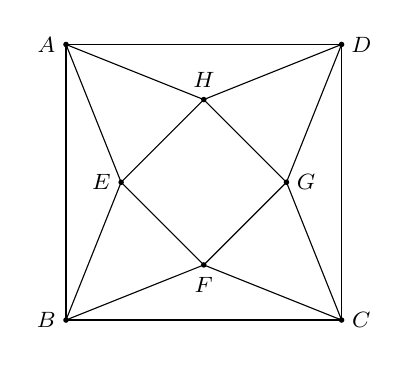
\begin{tikzpicture}[>=stealth,line join=round,line cap=round,font=\footnotesize,scale=1,declare function={a=3.5;r=a/sqrt(2);}]
			\foreach \i[count=\x] in {A,B,C,D}
			\path({45+\x*90}:r)coordinate(\i);
			\foreach \i[count=\x] in {E,F,G,H}
			\path({90+\x*90}:0.3*a)coordinate(\i);
			\draw (A)--(B)--(C)--(D)--cycle;
			\draw (E)--(F)--(G)--(H)--cycle;
			\draw (H)--(A)--(E)--(B)--(F)--(C)--(G)--(D)--cycle;
			\foreach \i\g in {A/180,B/180,C/0,D/0,E/180,F/-90,G/0,H/90}\fill(\i)circle(1pt)+(\g:.25)node{$\i$};
		\end{tikzpicture}
	}
	\choice
	{\True $\dfrac{4 \sqrt{10}}{3}$}
	{$\dfrac{4 \sqrt{10}}{5}$}
	{$\dfrac{8 \sqrt{10}}{3}$}
	{$\dfrac{8 \sqrt{10}}{5}$}
	\loigiai{
		\centerline{
			\begin{tikzpicture}[>=stealth,line join=round,line cap=round,font=\footnotesize,scale=1,declare function={a=4;r=a/sqrt(2);h=4.5;}]
				\tikzset{
					hv/.pic={\foreach \i[count=\x] in {A,B,C,D}
						\path({45+\x*90}:r)coordinate(\i);
						\foreach \i[count=\x] in {E,F,G,H}
						\path({90+\x*90}:0.3*a)coordinate(\i);
						\path 
						(0,0)coordinate(O)
						($(A)!1/2!(D)$)coordinate(K)
						;
						\draw (A)--(B)--(C)--(D)--cycle;
						\draw (E)--(F)--(G)--(H)--cycle (H)--(K);
						\draw (H)--(A)--(E)--(B)--(F)--(C)--(G)--(D)--cycle;
						\foreach \i\g in {A/180,B/180,C/0,D/0,E/180,F/-90,G/0,H/-90,O/0,K/90}\fill(\i)circle(1pt)+(\g:.25)node{$\i$};
						\path(H)--(K)node[midway,right]{$x$};},
					hchop/.pic={
						\path 	(0:0) coordinate (E)
						++(0:a) coordinate (H)
						++(-130:a/2) coordinate (G)
						($(E)+(G)-(H)$) coordinate (F)
						(intersection of E--G and H--F) coordinate (O)
						($(O)+(90:h)$) coordinate (S);
						\draw[dashed,thick] (O)--(S)--(E)--(G)	 (F)--(E)--(H)--(F);
						\draw[thick] (S)--(F)--(G)--(S)--(H)--(G);
						\foreach \x/\g in {S/90,O/-90,E/170,F/180,G/-90,H/0}
						\fill[black] 	(\x) circle (1.5pt)+(\g:3mm) node {$\x$};
					},
				}
				\path (0,1)pic{hv}
				(6,0)pic{hchop};
			\end{tikzpicture}
		}
		Gọi $K$ là trung điểm $A D$, đặt $H K=x, 0<x \leq \dfrac{5}{2}$.\\
		Ta có $E F=F G=G H=H E=\left(\dfrac{5}{2}-x\right) \sqrt{2}; H D=\sqrt{\left(\dfrac{5}{2}\right)^2+x^2}$.\\
		Suy ra $S O=\sqrt{S H^2-O H^2}=\sqrt{H D^2-O H^2}=\sqrt{\left(\dfrac{5}{2}\right)^2+x^2-\left(\dfrac{5}{2}-x\right)^2}$.\\
		Ta có $V=\dfrac{1}{3}\cdot 2 \cdot\left(\dfrac{5}{2}-x\right)^2 \sqrt{\left(\dfrac{5}{2}\right)^2+x^2-\left(\dfrac{5}{2}-x\right)^2}=\dfrac{2}{3}\cdot\left(\dfrac{5}{2}-x\right)^2 \cdot \sqrt{5 x}$.\\
		$\Rightarrow V'=\dfrac{2}{3}\left[-2\left(\dfrac{5}{2}-x\right) \sqrt{5 x}+\left(\dfrac{5}{2}-x\right)^2 \dfrac{5}{2 \sqrt{5 x}}\right], V'=0 \Leftrightarrow\left[\begin{aligned}
			&x=\dfrac{5}{2}\\ 
			&x=\dfrac{1}{2}\\
		\end{aligned}\right.$.\\
		Bảng biến thiên
		\begin{center}
			
\begin{tikzpicture}
				\tkzTabInit[nocadre,lgt=1,espcl=3]
				{$x$/1,$V'$/0.8,$V$/2.5}{$0$,$\dfrac{1}{2}$,$\dfrac{5}{2}$}
				\tkzTabLine{,+,0,-,}
				\tkzTabVar{-/{},+/$\dfrac{4\sqrt{10}}{3}$,-/{}}
			\end{tikzpicture}
		\end{center}
		Dựa vào bảng biến thiên, ta thấy $V_{\max}=\dfrac{4 \sqrt{10}}{3}$ khi $x=\dfrac{1}{2}$.
	}
\end{ex}

\begin{ex}%[2H1G3-6]
	Cho khối lập phương $ABCD.A'B'C'D'$ cạnh $a$ . Các điểm $M,N$ lần lượt di động trên các tia $AC,B'D'$ sao cho $AM+B'N=a\sqrt{2}$ .Thể tích khối tứ diện $AMNB'$ có giá trị lớn nhất là
	\choice
	{\True $\dfrac{a^3}{12}$}
	{$\dfrac{a^3}{6}$}
	{$\dfrac{a^3\sqrt{3}}{6}$}
	{$\dfrac{a^3\sqrt{2}}{12}$}
	\loigiai{
		\centerline{
			\begin{tikzpicture}[line join=round,line cap=round,font=\footnotesize,scale=1]
				\def\a{4}
				\def\b{2}
				\def\h{3}
				\path
				(0,0)coordinate (A)
				(0:\a)coordinate (B)
				(-150:\b)coordinate (D)
				($(D)+(B)-(A)$)coordinate (C)
				($(A)+(90:\h)$)coordinate (A')
				($(D)+(A')-(A)$)coordinate (D')
				($(C)+(A')-(A)$)coordinate (C')
				($(B)+(A')-(A)$)coordinate (B')
				($(B')!1/3!(D')$)coordinate (N)
				($(C)!1/3!(A)$)coordinate (M)
				;
				\draw  (B')--(A')--(D')--(D)--(C)--(B)--(B')--(C')--(C) (A')--(C')--(D')--(B');
				\draw[dashed] (B)--(A)--(D) (A')--(A)--(N)--(M)--(B')--(A)--(C)
				;
				\foreach \i \g in{A/175,B/0,C/-90,D/-90,A'/90,B'/90,C'/90,D'/180,M/-150,N/110}
				\fill (\i)circle(1pt)+(\g:2.5mm)node{$ \i $};
			\end{tikzpicture}
		}
		Ta có $V_{A{B}'MN}=\dfrac{1}{3}d\left(N,\left(A{B}'M\right)\right).S_{\Delta A{B}'M}$.\\
		Do $AC{B}'{D}'$ là tứ diện đều nên $\sin\left(\widehat{B'{D}',\left(A{B}'M\right)}\right)=\dfrac{\sqrt{6}}{3}$, $\sin\widehat{B'AM}=\dfrac{\sqrt{3}}{2}$.\\
		Suy ra $V_{A{B}'MN}=\dfrac{1}{3}\left(B'N.\sin\left(\widehat{B'{D}',\left(A{B}'M\right)}\right)\right).\dfrac{1}{2}A{B}'.AM.\sin\widehat{B'AM}=\dfrac{a}{6}.AM.B'N$\\
		$\le\dfrac{a}{6}{\left(\dfrac{AM+B'N}{2}\right)^2}=\dfrac{a^3}{12}$\\
		Vậy $\left(V_{A{B}'MN}\right)_{\max}=\dfrac{a^3}{12}$.
	}
\end{ex}

\begin{ex}%[2H1G3-6]%[Sở Bắc Ninh - 2019]
	Cho tứ diện $SABC$ có $G$ là trọng tâm tứ diện, mặt phẳng quay quanh $AG$ cắt các cạnh $SB,SC$ lần lượt tại $M,N$ . Giá trị nhỏ nhất của tỉ số $\dfrac{V_{S.AMN}}{V_{S.ABC}}$ là?
	\choice
	{\True $\dfrac{4}{9}$}
	{$\dfrac{3}{8}$}
	{$\dfrac{1}{3}$}
	{$\dfrac{1}{2}$}
	\loigiai{
		\centerline{
			\begin{tikzpicture}[>=stealth,line join=round,line cap=round,font=\footnotesize,scale=1,declare function={a=2;b=4;c=3;}]
				\tikzset{
					markx/.pic={\draw (45:.1)--(-135:.1) (-45:.1)--(135:.1);},
					markl/.pic={\draw (90:.1)--(-90:.1);},
				}
				\path
				(0,0)coordinate(A)
				(-40:a)coordinate(B)
				(b,0)coordinate(C)
				(b/2,c)coordinate(S)
				($(B)!1/2!(C)$)coordinate (E)
				($(S)!1/2!(A)$)coordinate (F)
				($(E)!1/2!(F)$)coordinate (G)
				(intersection of A--G and S--E)coordinate (I)
				($(S)!.55!(C)$)coordinate (N)
				(intersection of N--I and S--B)coordinate (M)
				;
				\draw (E)--(S)--(A)--(B)--(S)--(C)--(B) (A)--(M)--(N);
				\draw[dashed] (A)--(C) (N)--(A)--(I)
				(A)--(E)--(F)
				;
				\path (S)--(A)pic[pos=.25,rotate=-20]{markx}pic[pos=.75,rotate=-20]{markx};
				\path (B)--(C)pic[pos=.25,rotate=20]{markl}pic[pos=.75,rotate=20]{markl};
				\foreach \i \g in {A/180,B/-90,C/0,S/90,M/-150,N/40,I/0,G/80,E/-30,F/110}\fill(\i)circle(1pt)+(\g:.25)node[scale=.8]{$\i$};
				\begin{scope}[xshift=6cm]
					\path
					(0,0)coordinate(B)
					(b,0)coordinate(C)
					(70:c)coordinate(S)
					($(B)!1/2!(C)$)coordinate (E)
					($(S)!2/3!(E)$)coordinate (I)
					($(B)!1/6!(S)$)coordinate (M)
					(intersection of I--M and S--C)coordinate (N)
					($(I)!-1/5!(S)$)coordinate (P)
					($2*(E)-(P)$)coordinate (Q)
					;
					\draw (S)--(B)--(C)--(S)--(Q)--(C)
					(B)--(P)
					(M)--(N)
					;
					\path (B)--(C)pic[pos=.25,rotate=20]{markl}pic[pos=.75,rotate=20]{markl};
					\foreach \i \g in {B/180,C/0,S/90,M/150,N/40,I/45,P/10,E/-130,Q/-90}\fill(\i)circle(1pt)+(\g:.25)node[scale=.8]{$\i$};
				\end{scope}
				\begin{scope}[xshift=12cm]
					\path
					(0,0)coordinate(A)
					(c,0)coordinate(E)
					(60:b)coordinate(S)
					($(S)!2/3!(E)$)coordinate (I)
					($(S)!1/2!(A)$)coordinate (F)
					($(S)!1/4!(A)$)coordinate (K)
					(intersection of I--A and E--F)coordinate (G)
					;
					\draw (S)--(A)--(E)--(S)
					(A)--(I)
					(F)--(E)
					(K)--(G)
					;
					\path (F)--(E)pic[pos=.25,rotate=-20]{markx}pic[pos=.75,rotate=-20]{markx};
					\foreach \i \g in {S/90,A/180,E/0,G/-90,I/20,F/120,K/120}\fill(\i)circle(1pt)+(\g:.25)node[scale=.8]{$\i$};
				\end{scope}
			\end{tikzpicture}	
		}	
		Gọi $E,F,G$ lần lượt là trung điểm $BC,SA,EF$ suy ra $G$ là trọng tâm tứ diện $SABC$. Điểm $I$ là giao điểm của $AG$ và $SE$. Qua $I$ dựng đường thẳng cắt các cạnh $SB,SC$ lần lượt tại $M,N$. Suy ra $\left(AMN\right)$ là mặt phẳng quay quanh $AG$ thỏa mãn yêu cầu bài toán.\\
		Kẻ $GK\parallel SE,\left(K\in SA\right)$ suy ra $K$ là trung điểm $FS$.\\
		$\Rightarrow\dfrac{KG}{SI}=\dfrac{AK}{AS}=\dfrac{3}{4}$. Mà $\dfrac{KG}{SE}=\dfrac{1}{2}\Rightarrow\dfrac{SI}{SE}=\dfrac{2}{3}$.
		\begin{itemize}
			\item Cách 1\\
			Kẻ $BP\parallel MN,CQ\parallel MN$ ; $\left(P,Q\in SE\right)$.\\
			Ta có $\dfrac{SM}{SB}=\dfrac{SI}{SP};\dfrac{SN}{SC}=\dfrac{SI}{SQ}$ .\\
			$\Rightarrow\Delta BEP=\Delta CEQ$ $\Rightarrow $ $E$ là trung điểm $PQ$ $\Rightarrow SP+SQ=2SE$ (đúng cả trong trường hợp $P\equiv Q\equiv E$).\\
			Ta có $\dfrac{V_{S.AMN}}{V_{S.ABC}}=\dfrac{SA}{SA}.\dfrac{SM}{SB}.\dfrac{SN}{SC}=1.\dfrac{SI}{SP}.\dfrac{SI}{SQ}\overset{AM-GM}{\mathop{\ge}}\dfrac{S{I^2}}{\frac{\left(SP+SQ\right)^2}{4}}=\dfrac{S{I^2}}{S{E^2}}=\left(\dfrac{SI}{SE}\right)^2=\dfrac{4}{9}$.\\
			Dấu ``$=$'' xảy ra khi và chỉ khi $SP=SQ=SE$. Hay $P\equiv Q\equiv E\Leftrightarrow MN\parallel BC$.
			\item Cách 2\\
			Ta chứng minh được $\dfrac{SB}{SM}+\dfrac{SC}{SN}=3$.\\
			\centerline{
				\begin{tikzpicture}[>=stealth,line join=round,line cap=round,font=\footnotesize,scale=1,declare function={b=5;c=3;}]
					\path
					(0,0)coordinate(B)
					(b,0)coordinate(C)
					(70:c)coordinate(S)
					($(B)!1/2!(C)$)coordinate (E)
					($(S)!2/3!(E)$)coordinate (I)
					($(B)!2/5!(S)$)coordinate (M)
					(intersection of I--M and S--C)coordinate (N)
					(intersection of I--B and S--C)coordinate (D)
					(intersection of I--C and S--B)coordinate (L)
					;
					\coordinate (Q1) at ($(S)+(I)-(B)$); 
					\coordinate (Q) at (intersection of I--Q1 and C--S);
					\coordinate (P1) at ($(S)+(I)-(C)$); 
					\coordinate (P) at (intersection of I--P1 and B--S);
					\draw (S)--(B)--(C)--(S)--(E)
					(B)--(D)
					(C)--(L)
					(M)--(N)
					(P)--(I)--(Q)
					;
					\foreach \i \g in {B/180,C/0,S/90,M/-150,N/40,I/-100,P/130,E/-90,Q/60,L/160,D/50}\fill(\i)circle(1pt)+(\g:.25)node[scale=.8]{$\i$};
				\end{tikzpicture}
			}
			Thật vậy, qua $I$ kẻ các đường thẳng lần lượt song song $SB,SC$ cắt $SC,SB$ tương ứng tại $D,L$.\\
			Ta có $\left.\begin{aligned}
				&\dfrac{SB}{IQ}=\dfrac{DB}{DI}=3\\ 
				&\dfrac{IQ}{SM}=\dfrac{NI}{NM}\\ 
			\end{aligned}\right\}\Rightarrow\dfrac{SB}{IQ}.\dfrac{IQ}{SM}=3.\dfrac{NI}{NM}\Leftrightarrow\dfrac{SB}{SM}=\dfrac{3NI}{NM}$, $(1)$.\\
			Lại có $\left.\begin{aligned}
				&\dfrac{SC}{IP}=\dfrac{LC}{LI}=3\\ 
				&\dfrac{IP}{SN}=\dfrac{MI}{MN}\\ 
			\end{aligned}\right\}\Rightarrow\dfrac{SC}{IP}.\dfrac{IP}{SN}=3.\dfrac{MI}{MN}\Leftrightarrow\dfrac{SC}{SN}=\dfrac{3MI}{MN}$, $(2)$.\\
			Từ $(1)$ và $(2)$ ta có $\dfrac{SB}{SM}+\dfrac{SC}{SN}=3\left(\dfrac{NI}{NM}+\dfrac{MI}{MN}\right)=3$.\\
			Đặt $x=\dfrac{SB}{SM};y=\dfrac{SC}{SN}$. Suy ra $x+y=3$.\\
			Ta có $\dfrac{V_{S.AMN}}{V_{S.ABC}}=\dfrac{SA}{SA}.\dfrac{SM}{SB}.\dfrac{SN}{SC}=\dfrac{1}{xy}\overset{AM-GM}{\mathop{\ge}}\dfrac{1}{\frac{\left(x+y\right)^2}{4}}=\dfrac{4}{9}$.\\
			Dấu ``$=$'' xảy ra khi và chỉ khi $x=y=\dfrac{3}{2}\Leftrightarrow MN\parallel BC$.
			\item Cách 3\\
			Đặt $\dfrac{SB}{SM}=x$; $\dfrac{SC}{SN}=y$, với $ x>0$, $ y>0$.\\
			Ta có $\overrightarrow{SI}=\dfrac{2}{3}\overrightarrow{SE}=\dfrac{1}{3}(\overrightarrow{SB}+\overrightarrow{SC})=\dfrac{1}{3}(x\overrightarrow{SM}+y\overrightarrow{SN})=\dfrac{x}{3}\overrightarrow{SM}+\dfrac{y}{3}\overrightarrow{SN}$.\\
			Do $I$, $M$, $N$ thẳng hàng nên $\dfrac{x}{3}+\dfrac{y}{3}=1\Leftrightarrow x+y=3$.\\
			Ta có $\dfrac{V_{S.AMN}}{V_{S.ABC}}=\dfrac{SM}{SB}.\dfrac{SN}{SC}=\dfrac{1}{x}\cdot\dfrac{1}{y}=\dfrac{1}{xy}\ge\dfrac{1}{(\frac{x+y}{2})^2}=\dfrac{4}{9}$ .\\
			Vậy $\dfrac{V_{S.AMN}}{V_{S.ABC}}$ đạt giá trị nhỏ nhất bằng $\dfrac{4}{9}$ khi $x=y$, hay $MN$ đi qua $I$ và song song với $BC$.
		\end{itemize}	
	}
\end{ex}
%Câu 18
\begin{ex}%[2H1G3-6]
	[Chuyên Biên Hòa - Hà Nam - 2020]
	Cho hình chóp $ S.ABCD$ có đáy $ ABCD$ là hình bình hành. Hai điểm $M$, $ N$ lần lượt thuộc các đoạn thẳng $ AB$ và $ AD$ ($ M$ và $ N$ không trùng với $ A$) sao cho $ 2\dfrac{AB}{AM}+3\dfrac{AD}{AN}=8$. Kí hiệu $ V$, $V_1$ lần lượt là thể tích của các khối chóp $ S.ABCD$ và $ S.MBCDN$. Tìm giá trị lớn nhất của tỉ số $\dfrac{V_1}{V}$.
	\choice
	{\True $\dfrac{13}{16}$}
	{$\dfrac{11}{12}$}
	{$\dfrac{1}{6}$}
	{$\dfrac{2}{3}$}
	\loigiai{
		\begin{center}
			\begin{tikzpicture}[line join=round, line cap=round,thick]
				\coordinate (A) at (-3,-2);
				\coordinate (B) at (2,-2);
				\coordinate (D) at (0,0);
				\coordinate (C) at ($(B)+(D)-(A)$);
				\coordinate (M) at ($(A)!0.5!(B)$);
				\coordinate (N) at ($(A)!0.7!(D)$);
				\coordinate (S) at ($(M)+(0,5)$);
				\draw(S)--(A) (S)--(B) (S)--(C) (A)--(B) (B)--(C) (S)--(M);
				\draw[dashed,thin] (A)--(D) (D)--(C) (N)--(M) (D)--(B) (S)--(N) (S)--(D);
				\foreach \i/\g in {S/90,A/-90,B/-90,C/-90,D/180,M/-90, N/180}{\draw[fill=white](\i) circle (1pt) ($(\i)+(\g:3mm)$) node[scale=1]{$\i$};}
			\end{tikzpicture}
		\end{center}
		Ta có $\dfrac{V_{SADB}}{V_{SANM}}=\dfrac{AD}{AN}\cdot\dfrac{AB}{AM}\Leftrightarrow\dfrac{2.V_{SADB}}{V_{SANM}}=2\cdot\dfrac{AD}{AN}\cdot\dfrac{AB}{AM}$\\
		$\Leftrightarrow\dfrac{V}{V-V_1}=2\cdot\dfrac{AD}{AN}\cdot\dfrac{AB}{AM}\Leftrightarrow\dfrac{V-V_1}{V}=\dfrac{1}{2.\dfrac{AD}{AN}\cdot\dfrac{AB}{AM}}\Leftrightarrow\dfrac{V_1}{V}=\dfrac{2\cdot\dfrac{AD}{AN}\cdot\dfrac{AB}{AM}-1}{2\cdot\dfrac{AD}{AN}\cdot\dfrac{AB}{AM}}$\\
		Đặt $ x=\dfrac{AD}{AN}\Rightarrow 2\dfrac{AB}{AM}=8-3x,\left(1\le x\le 2\right)$. Khi đó $\dfrac{V_1}{V}=\dfrac{x\left(8-3x\right)-1}{x\left(8-3x\right)}=1+\dfrac{1}{3x^2-8x}$\\
		Đặt $ f(x)=1+\dfrac{1}{3x^2-8x},\left(1\le x\le 2\right)$\\
		Ta có: $f'(x)=-\dfrac{6x-8}{\left(3x^2-8x\right)^2}$$\Rightarrow{f}'(x)=0\Leftrightarrow-\dfrac{6x-8}{\left(3x^2-8x\right)^2}=0\Leftrightarrow x=\dfrac{4}{3}\Rightarrow f\left(\dfrac{4}{3}\right)=\dfrac{13}{16}$\\
		Bảng biến thiên hàm số $y=f(x)$
		\begin{center}
			
\begin{tikzpicture}
				\tkzTabInit[nocadre,lgt=1.2,espcl=3,deltacl=0.6]
				{$x$/1,$f'(x)$/0.7,$f(x)$/2.5}{$1$,$\dfrac{4}{3}$,$2$}
				\tkzTabLine{,+,0,-,}
				\tkzTabVar{-/$\dfrac{4}{5}$,+/$\dfrac{13}{16}$,-/$\dfrac{3}{4}$}
			\end{tikzpicture}
		\end{center} 
		Dựa vào bảng biến thiên ta được hàm số đạt giá trị lớn nhất là $\dfrac{13}{16}$ tại $ x=\dfrac{4}{3}$.\\
		Vậy giá trị lớn nhất của tỉ số $\dfrac{V_1}{V}$ là $\dfrac{13}{16}$.
	}
\end{ex} 
% Câu 19
\begin{ex}%[2H1G3-6]
	[Chuyên ĐH Vinh - Nghệ An - 2020]
	Cho hình chóp $ S.ABCD$ có đáy $ ABCD$ là hình bình hành và có thể tích là $ V$. Gọi $ P$ là trung điểm của $ SC$. Mặt phẳng $\left(\alpha\right)$ chứa $ AP$ và cắt hai cạnh $ SD$, $ SB$ lần lượt tại $ M$ và $ N$. Gọi $V'$ là thể tích của khối chóp $ S.AMPN$. Tìm giá trị nhỏ nhất của tỉ số $\dfrac{V'}{V}$.
	\choice
	{$\dfrac{3}{8}$}
	{\True $\dfrac{1}{3}$}
	{$\dfrac{2}{3}$}
	{$\dfrac{1}{8}$}
	\loigiai{
		\begin{center}
			\begin{tikzpicture}[line join=round, line cap=round,thick]
				\coordinate (S) at (1,5);
				\coordinate (B) at (-3,-2);
				\coordinate (C) at (2,-2);
				\coordinate (A) at (0,0);
				\coordinate (D) at ($(A)+(C)-(B)$);
				\coordinate (N) at ($(S)!0.6!(B)$);
				\coordinate (P) at ($(S)!0.5!(C)$);
				\coordinate (M) at ($(S)!0.7!(D)$);
				\draw(S)--(B) (S)--(C) (S)--(D) (B)--(C) (C)--(D) (N)--(P) (P)--(M);
				\draw[dashed,thin] (S)--(A) (A)--(N) (A)--(P) (A)--(M) (A)--(B) (A)--(D);
				\foreach \i/\g in {S/90,A/-90,B/-90,C/-90,D/0,M/0, N/180, P/45}{\draw[fill=white](\i) circle (1pt) ($(\i)+(\g:3mm)$) node[scale=1]{$\i$};}
			\end{tikzpicture}
		\end{center}
		Do $\left(\alpha\right)$ đi qua $ A$, $ P$, $ M$, $ N$ nên bốn điểm này đồng phẳng.\\
		Áp dụng công thức $\dfrac{V_{S.AMNP}}{V_{S.ABCD}}=\dfrac{a+b+c+d}{4.a.b.c.d}$ với $\dfrac{SA}{SA}=a$, $\dfrac{SC}{SP}=c$,$\dfrac{SD}{SM}=d$, $\dfrac{SB}{SN}=b$\\
		thỏa mãn $ a+c=b+d$.\\
		Theo đề bài ta có $\dfrac{SA}{SA}=1$, $\dfrac{SC}{SP}=2$ và đặt $\dfrac{SD}{SM}=d>0$, $\dfrac{SB}{SN}=b>0$.\\
		Khi đó: $\dfrac{V'}{V}=\dfrac{1+2+b+d}{4.1.2.b.d}$ với $1+2=b+d\Leftrightarrow b+d=3$.\\
		Vậy ta có: $\dfrac{V'}{V}=\dfrac{1+2+b+d}{4.1.2.b.d}\Leftrightarrow\dfrac{V'}{V}=\dfrac{1+2+3}{4.2.b.d}\Leftrightarrow\dfrac{V'}{V}=\dfrac{3}{4bd}$.\\
		Theo bất đẳng thức cơ bản: $bd\le\dfrac{\left(b+d\right)^2}{4}=\dfrac{9}{4}\Leftrightarrow\dfrac{1}{bd}\ge\dfrac{4}{9}$ suy ra $\dfrac{V'}{V}=\dfrac{3}{4bd}\ge\dfrac{3}{4}.\dfrac{4}{9}=\dfrac{1}{3}$.\\
		Dấu “=” xảy ra $ b=d\Leftrightarrow b=d=\dfrac{3}{2}$.\\
		Vậy $\dfrac{V'}{V}$ có giá trị nhỏ nhất bằng $\dfrac{1}{3}$.
	}
\end{ex}

% Câu 20
\begin{ex}%[2H1G3-2]
	[Chuyên KHTN - 2020]
	Cho khối lăng trụ đứng $ ABC.A'{B}'{C}'$ có đáy $ ABC$ là tam giác vuông cân tại $ C$, $ AB=2a$ và góc tạo bởi hai mặt phẳng $\left(AB{C}'\right)$ và $\left(ABC\right)$ bằng $ 60^\circ $. Gọi $ M,N$ lần lượt là trung điểm của $A'{C}'$ và $ BC$. Mặt phẳng $\left(AMN\right)$ chia khối lăng trụ thành hai phần. Thể tích của phần nhỏ bằng
	\choice
	{\True $\dfrac{7\sqrt{3}{a^3}}{24}$}
	{$\dfrac{\sqrt{6}{a^3}}{6}$}
	{$\dfrac{7\sqrt{6}{a^3}}{24}$}
	{$\dfrac{\sqrt{3}{a^3}}{3}$}
	\loigiai{ 
	\textit{
		\begin{center}
			\begin{tikzpicture}[line cap=round, line join=round, font=\footnotesize, >=stealth, scale=0.8]
				\coordinate (C) at  (0,0) ;
				\coordinate (A) at (0.6,-1.8) ;
				\coordinate (B) at (5,0) ;
				\foreach \x in {A,B,C} {\coordinate (\x') at ($(\x)+(0,2.5)$);}
				\draw (C')--(A')--(B');
				\draw (C)--(A)--(B) (C)--(C') (A)--(A') (B)--(B') (C')--(A) ;
				\draw[dashed] (C)--(B);
				\coordinate (M) at ($(C')!0.5!(A')$);
				\coordinate (I) at ($(A)!0.5!(B)$);
				\coordinate (N) at ($(C)!0.5!(B)$);
				\coordinate (O) at (0,5);
				\draw (C) -- (O);
				\draw[dashed] (A)--(N) (C)--(I) (C')--(I) (C')--(B);
				\draw[dashed][name path=O--N] (O) -- (N);
				\draw[dashed][name path=C'--B'] (C') -- (B');				
				\path [name intersections={of=C'--B' and O--N,by=E}];				
				\draw (M)--(E) (E)--(B') (O)--(E) (A)--(O);
				\foreach \i/\g in {A/-90,B/-90,C/180,A'/0,B'/0,C'/180, M/180, I/90, N/90, O/90, E/90}{\draw[fill=white](\i) circle (1pt) ($(\i)+(\g:3mm)$) node[scale=1]{$\i$};}
			\end{tikzpicture}
		\end{center}	
		\textbf{Cách 1:}}\\
		Gọi $ I$ là trung điểm $ AB$, suy ra $ AB\perp\left(CI{C}'\right)$ nên góc giữa $\left(C'AB\right)$ và $\left(ABC\right)$ là góc $\left(CI,C'I\right)$, suy ra $\widehat{C'IC}=60^\circ $.\\
		Tam giác $C'IC$ vuông tại $ C$ nên $C'C=CI\cdot\tan\widehat{C'IC}=\dfrac{AB}{2}\cdot\tan 60^\circ=a\sqrt{3}$.\\
		Diện tích tam giác $ ABC$ là $S_{ABC}=\dfrac{1}{2}\cdot AB\cdot CI=a^2$.\\
		Thể tích khối lăng trụ là $V=C{C}'\cdot{S_{ABC}}=a\sqrt{3}\cdot{a^2}=a^3\sqrt{3}$.\\
		Trong $\left(AC{C}'{A}'\right)$, kéo dài $ AM$ cắt $ C{C}'$ tại $O$.\\
		Suy ra $C'M$ là đường trung bình của $\Delta OAC$, do đó $OC=2C{C}'=2a\sqrt{3}$.\\
		Thể tích khối chóp $V_{O.ACN}=\dfrac{1}{3}\cdot{S_{ACN}}\cdot OC=\dfrac{1}{3}\cdot\dfrac{1}{2}\cdot{S_{ABC}}\cdot 2C{C}'=\dfrac{1}{3}V$.\\
		Thể tích khối chóp $V_{O.C'ME}=\dfrac{1}{3}\cdot{S_{C'ME}}\cdot O{C}'=\dfrac{1}{3}\cdot\dfrac{1}{8}{S_{A'{B}'{C}'}}\cdot O{C}'=\dfrac{1}{24}V$.\\
		Do đó $V_{C'EM.CAN}=V_{O.ACN}-V_{O.C'ME}=\dfrac{1}{3}V-\dfrac{1}{24}V=\dfrac{7}{24}V=\dfrac{7}{24}\cdot{a^3}\sqrt{3}=\dfrac{7\sqrt{3}{a^3}}{24}$.\\
		Vậy phần thể tích nhỏ hơn là $V_{C'EM.CAN}=\dfrac{7\sqrt{3}{a^3}}{24}$.\\
		\textit{\textbf{Cách 2:}}\\
		Kẻ $ ME\parallel AN$\\
		Góc tạo bởi $\left(ABC'\right)$ và $\left(ABC\right)$ là góc $\widehat{C'IC}=60^0$ với $ I$ là trung điểm $ AB$.\\
		$ CC'=CI.\tan{60^\circ}=a\sqrt{3}$\\
		$S_{ABC}=\dfrac{1}{2}CI\cdot AB=a^2$\\
		$S_1=S_{ACN}=\dfrac{1}{2}{S_{ABC}}=\dfrac{1}{2}{a^2}$\\
		$S_2=S_{C'ME}=\dfrac{1}{4}{S_{ABC}}=\dfrac{1}{2}C'M\cdot C'E=\dfrac{1}{8}{a^2}$\\
		$V=\dfrac{CC'}{3}\left(S_1+S_2+\sqrt{S_1S_2}\right)=\dfrac{7\sqrt{3}{a^3}}{24}$.}
\end{ex}

%Cau 21
\begin{ex}[Chuyên Phan Bội Châu - Nghệ An - 2020]%[2H1T3-2]
	Cho một tấm nhôm hình vuông cạnh $ 12$ $\mathrm{cm}$. Người ta cắt ở bốn góc của tấm nhôm đó bốn hình vuông bằng nhau, mỗi hình vuông có cạnh bằng $x$ ($\mathrm{cm}$), rồi gập tấm nhôm lại để được một cái hộp không nắp (tham khảo hình vẽ bên). Tìm $ x$ để hộp nhận được có thể tích lớn nhất (giả thiết bề dày tấm tôn không đáng kể).\\
	\centerline{
		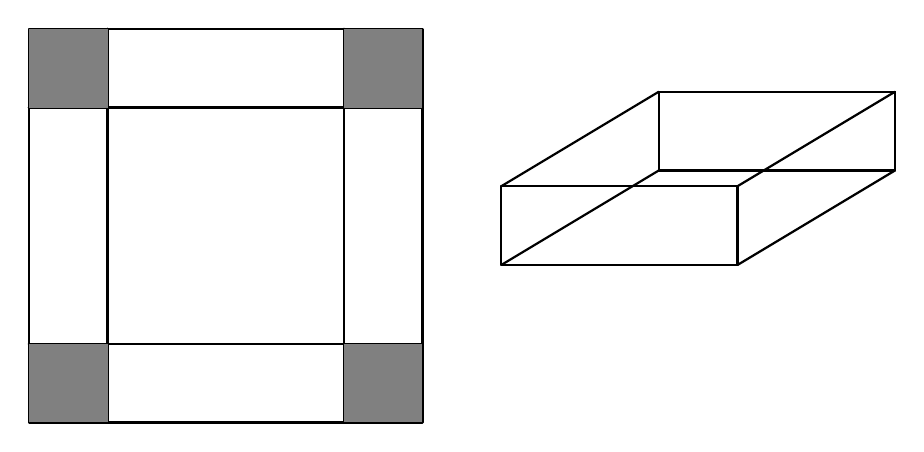
\begin{tikzpicture}[line join=round,line cap=round,font=\footnotesize,scale=1]
				\begin{scope}[xshift=8cm]
				\coordinate (A) at (0,0);
				\coordinate (B) at (5,0);
				\coordinate (C) at (5,5);
				\coordinate (D) at (0,5);
				
				\coordinate (M) at (1,1);
				\coordinate (N) at (4,1);
				\coordinate (P) at (4,4);
				\coordinate (Q) at (1,4);
				
				\coordinate (E) at (1,0);
				\coordinate (F) at (4,0);
				\coordinate (G) at (5,1);
				\coordinate (H) at (5,4);
				\coordinate (I) at (4,5);
				\coordinate (J) at (1,5);
				\coordinate (K) at (0,4);
				\coordinate (L) at (0,1);
				
				\draw[thick] (E)--(J) (F)--(I) (G)--(L) (H)--(K);
				
				\draw[thick] (A)--(B)--(C)--(D)--cycle;
				\draw[thick] (M)--(N)--(P)--(Q)--cycle;
				\draw[thick] (M)--(N)--(P)--(Q)--cycle;
				
				%\foreach \x/\g in {A/135,B/-135,C/-45,D/45, M/-90, N/-90, P/90, Q/90};
				%\fill[grey] 	(\x) circle (1.5pt)+(\g:2.5mm) node {$\x$};	
				\fill[gray] (A)--(E)--(M)--(L)--cycle;
				\fill[gray] (F)--(B)--(G)--(N)--cycle;
				\fill[gray] (H)--(C)--(I)--(P)--cycle;
				\fill[gray] (J)--(Q)--(K)--(D)--cycle;
			\end{scope}
			\begin{scope}[xshift=14cm,yshift=2cm]
				\coordinate (A) at (0,0);
				\coordinate (B) at (3,0);
				\coordinate (C) at (3,1);
				\coordinate (D) at (0,1);
				
				\coordinate (M) at (2,1.2);
				\coordinate (N) at (5,1.2);
				\coordinate (P) at (5,2.2);
				\coordinate (Q) at (2,2.2);
				
				\draw[thick] (A)--(B)--(C)--(D)--cycle;
				\draw[thick] (M)--(N)--(P)--(Q)--cycle;
				\draw[thick] (A)--(M) (B)--(N) (C)--(P) (D)--(Q);
				\end{scope}
	\end{tikzpicture}
}
	\choice
	{\True $x=2$}
	{$x=3$}
	{$x=4$}
	{$x=6$}
	\loigiai{
		Hình hộp có đáy của là hình vuông cạnh bằng $12-2x$, chiều cao bằng $x$.\\
		Điều kiện $0<x<6$\\
		\centerline{
		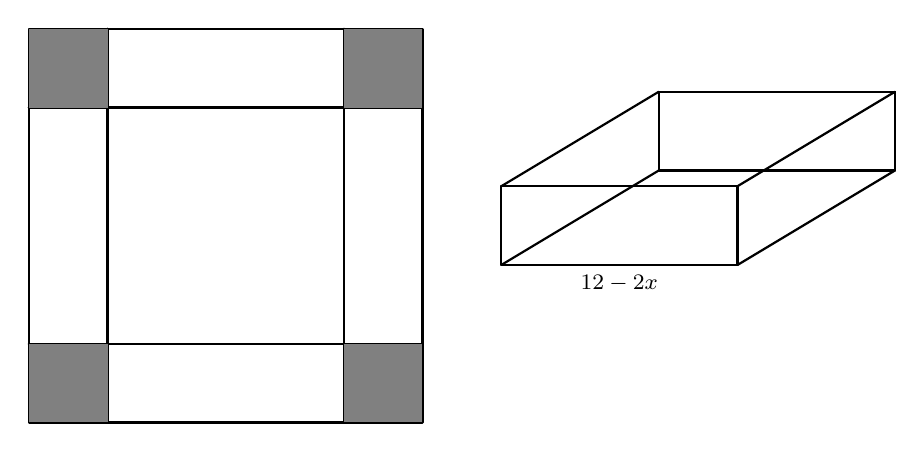
\begin{tikzpicture}[line join=round,line cap=round,font=\footnotesize,scale=1]
			\begin{scope}[xshift=8cm]
				\coordinate (A) at (0,0);
				\coordinate (B) at (5,0);
				\coordinate (C) at (5,5);
				\coordinate (D) at (0,5);
				
				\coordinate (M) at (1,1);
				\coordinate (N) at (4,1);
				\coordinate (P) at (4,4);
				\coordinate (Q) at (1,4);
				
				\coordinate (E) at (1,0);
				\coordinate (F) at (4,0);
				\coordinate (G) at (5,1);
				\coordinate (H) at (5,4);
				\coordinate (I) at (4,5);
				\coordinate (J) at (1,5);
				\coordinate (K) at (0,4);
				\coordinate (L) at (0,1);
				
				\draw[thick] (E)--(J) (F)--(I) (G)--(L) (H)--(K);
				
				\draw[thick] (A)--(B)--(C)--(D)--cycle;
				\draw[thick] (M)--(N)--(P)--(Q)--cycle;
				\draw[thick] (M)--(N)--(P)--(Q)--cycle;
				
				%\foreach \x/\g in {A/135,B/-135,C/-45,D/45, M/-90, N/-90, P/90, Q/90};
				%\fill[grey] 	(\x) circle (1.5pt)+(\g:2.5mm) node {$\x$};	
				\fill[gray] (A)--(E)--(M)--(L)--cycle;
				\fill[gray] (F)--(B)--(G)--(N)--cycle;
				\fill[gray] (H)--(C)--(I)--(P)--cycle;
				\fill[gray] (J)--(Q)--(K)--(D)--cycle;
			\end{scope}
			\begin{scope}[xshift=14cm,yshift=2cm]
				\coordinate (A) at (0,0);
				\coordinate (B) at (3,0);
				\coordinate (C) at (3,1);
				\coordinate (D) at (0,1);
				
				\coordinate (M) at (2,1.2);
				\coordinate (N) at (5,1.2);
				\coordinate (P) at (5,2.2);
				\coordinate (Q) at (2,2.2);
				
				\draw[thick] (A)--(B)--(C)--(D)--cycle;
				\draw[thick] (M)--(N)--(P)--(Q)--cycle;
				\draw[thick] (A)--(M) (B)--(N) (C)--(P) (D)--(Q);
				\path (A)--(B)node[pos=.5,below]{$12-2x$};
			\end{scope}
		\end{tikzpicture}
	}
		Thể tích khối hộp là $V=\left(12-2x\right)^2.x=4\left(6-x\right)^2x$.\\
		Áp dụng bất đẳng thức Cauchy cho 3 số dương $\sqrt[3]{\left(6-x\right)\left(6-x\right).2x}\le\dfrac{\left(6-x\right)+\left(6-x\right)+2x}{3}$\\
		$\Leftrightarrow\left(6-x\right)\left(6-x\right).2x\le{4^3}$ $\Leftrightarrow 4\left(6-x\right)^2.x\le{2.4^3}$ $\Leftrightarrow V\le 128$ (hằng số).\\
		Dấu ``$=$'' xảy ra $\Leftrightarrow 6-x=2x$ $\Leftrightarrow x=2$.\\
		Vây thể tích khối hộp lớn nhất khi $x=2$.}
	
	
\end{ex}

% Câu 22
\begin{ex}[Chuyên Phan Bội Châu - Nghệ An - 2020]%[2H1T3-6]
	Cho hình chóp $S.ABC$ có thể tích bằng $1$. Mặt phẳng $(Q)$ thay đổi song song với mặt phẳng $(ABC)$ lần lượt cắt các cạnh $SA$, $SB$, $SC$ tại $M$, $N$, $P$. Qua $M$, $N$, $P$ kẻ các đường thẳng song song với nhau lần lượt cắt mặt phẳng $(ABC)$ tại $M'$, $N'$, $P'$. Tính giá trị lớn nhất của thể tích khối lăng trụ $MNP.M'N'P'$.
	\choice
	{\True $\dfrac{4}{9}$}
	{$\dfrac{1}{3}$}
	{$\dfrac{1}{2}$}
	{$\dfrac{8}{27}$}
	\loigiai{
		\begin{center}
			\begin{tikzpicture}[line join=round,line cap=round,font=\footnotesize,scale=1,declare function={h=7;r=h/sqrt(3);}]
				\path 
				(0,0)coordinate(A)
				(h,0)coordinate(C)
				(-30:2*h/3)coordinate(B)
				($(B)!0.5!(C)$)coordinate(K)
				($(A)!0.5!(K)$)coordinate(H)
				($(H)+(90:h)$)coordinate(S)	
				($(S)!0.5!(C)$)coordinate(P)	
				($(S)!0.5!(A)$)coordinate(M)
				($(S)!0.5!(B)$)coordinate(N)
				($(A)!0.5!(H)$)coordinate(H')
				($(A)!1/3!(C)$)coordinate(I)
				($(I)!1/3!(H)$)coordinate(M')
				($(M')+(N)-(M)$)coordinate(N')
				($(N')+(P)-(N)$)coordinate(P')
				;
				\draw (S)--(C)--(B)--(A)--cycle;
				\draw (S)--(B) (M)--(N) (N)--(P) ;
				\draw[dashed] (A)--(C) (S)--(H) (M)--(P) (A)--(H) (M)--(H') (M)--(M') (M')--(N') (N')--(P') (P')--(P) (M')--(P') (N)--(N') ;
				\foreach \i\g in{S/90,A/180,B/-90,C/0,M/180,H/-90,N/-30, P/0, H'/-90,M'/180, N'/0, P'/0}\draw[fill=white](\i)circle(1pt)+(\g:2.5mm)node{$ \i $};
			\end{tikzpicture}
		\end{center}
		Gọi $\dfrac{SM}{SA}=x\left(0<x<1\right)$$\Rightarrow\dfrac{SN}{SB}=x=\dfrac{SP}{SC}$\\
		$\Rightarrow $$\dfrac{S_{\Delta MNP}}{S_{\Delta ABC}}=\dfrac{\tfrac{1}{2}NM\cdot NP\cdot \sin\widehat{MNP}}{\tfrac{1}{2}BA\cdot BC\cdot\sin\widehat{ABC}}=\dfrac{NM}{BA}\cdot\dfrac{NP}{BC}=x^2$.\\
		$\Rightarrow S_{\Delta MNP}=x^2.S_{\Delta ABC}$.\\
		Gọi chiều cao của hình chóp là $ SH$, chiều cao của lăng trụ là $M{H}'$\\
		$\Rightarrow $$\dfrac{M{H}'}{SH}=\dfrac{AM}{AS}=1-x\Rightarrow $$ MH'=\left(1-x\right)SH$\\
		$\Rightarrow V_{S.ABC}=\dfrac{1}{3}SH\cdot S_{\Delta ABC}=1\Leftrightarrow SH.S_{\Delta ABC}=3$\\
		$\Rightarrow V_{MNP.M'N'P'}=MH'.S_{\Delta MNP}=\left(1-x\right)SH.x^2.S_{\Delta ABC}=x^2.\left(1-x\right).SH.S_{\Delta ABC}$=$x^2.\left(1-x\right).3$\\
		Xét hàm số: $ f(x)=3x^2-3x^3$ với $ x\in\left(0;1\right)$\\
		$\Rightarrow f'(x)=6x-9x^2\Rightarrow f'(x)=0\Leftrightarrow\left[\begin{aligned}
			& x=0~(\text{loại})\\ 
			& x=\dfrac{2}{3}\\ 
		\end{aligned}\right.$\\
		Bảng biến thiên:
		\begin{center}
			
\begin{tikzpicture}
				\tkzTabInit[nocadre,lgt=1.2,espcl=3]{$x$/1.0,$f'(x)$/0.8,$f(x)$/2.5}{$0$,$\dfrac{2}{3}$,$1$}
				\tkzTabLine{,+,0,-,}
				\tkzTabVar{-/{},+/$\dfrac{4}{9}$,-/{}}
			\end{tikzpicture}
		\end{center}
		Vậy: $\max{{V}_{MNP.M'N'P'}}=\dfrac{4}{9}$.
	}
\end{ex}

%câu 23
\begin{ex}[Chuyên Vĩnh Phúc - 2020]%[2H1T3-6]
	Cho hình vuông $ ABCD$ cạnh $ a$. Trên đường thẳng vuông góc với $\left(ABCD\right)$ tại $ A$ lấy điểm $ S$ di động không trùng với $ A$. Hình chiếu vuông góc của $ A$ lên $ SB,SD$ lần lượt tại $ H$, $ K$. Tìm giá trị lớn nhất của thể tích khối tứ diện $ ACHK$.
	\choice
	{$\dfrac{a^3\sqrt{6}}{32}$}
	{$\dfrac{a^3}{6}$}
	{\True $\dfrac{a^3\sqrt{3}}{16}$}
	{$\dfrac{a^3\sqrt{2}}{12}$}
	\loigiai{ 
	\textbf{\textit{Cách 1}}
	{\begin{center}
					\begin{tikzpicture}[line join=round,line cap=round,font=\footnotesize,scale=1]
					%\def\a{4}
					\def\b{6}
					\path 	(0:0) coordinate (A)
					(0:\b) coordinate (D)
					++(-150:\b/2)coordinate (C)
					($(A)+(C)-(D)$)coordinate(B)
					($(90: \b)$) coordinate (S)
					($(S)!0.5!(D)$)coordinate(K)
					($(S)!0.5!(B)$)coordinate(H)
					(intersection of A--C and B--D)coordinate(O)
					(intersection of H--K and S--O)coordinate(G)
					(intersection of A--G and S--C)coordinate(I)
					;
					\draw[dashed,thick] 	(A)--(B) (A)--(D) (S)--(A) (C)--(A) (B)--(D) (H)--(K) (S)--(O) (A)--(H) (A)--(K) (A)--(I)  ;
					\draw[thick] (S)--(B)--(C)--(D)--cycle;
					\draw[thick] (S)--(C) (H)--(C) (C)--(K);
					
					\foreach \i\g in{S/90,A/180,B/-90, C/-90,D/0, O/-90, H/180, K/0, G/-45, I/0}\draw[fill=white](\i)circle(1pt)+(\g:2.5mm)node{$ \i $};
				\end{tikzpicture}
				\end{center}
		đặt $S A=x>0$						
		Ta có $V_{S . A B D}=\dfrac{1}{3}S_{A B D}\cdot S A=\dfrac{a^2 x}{6}$.\\
		Lại có $\dfrac{V_{S . A H K}}{V_{S . A B D}}=\dfrac{S H}{S B}\cdot \dfrac{S K}{S D}=\left(\dfrac{S A}{S B}\right)^2 \cdot\left(\dfrac{S A}{S D}\right)^2=\dfrac{x^4}{\left(x^2+a^2\right)^2}$.\\
		$\Rightarrow V_{S.AHK}=\dfrac{x^4}{\left(x^2+a^2\right)^2}V_{S . A B D}=\dfrac{a^2 x^5}{6\left(x^2+a^2\right)^2}$.\\
		Gọi $O=A C \cap B D, G=S O \cap H K, I=A G \cap S C$.\\
		Ta có $\left\{\begin{aligned}
			&B C \perp A B \\ 
			&B C \perp S A\\
		\end{aligned}\Rightarrow B C \perp(S A B) \Rightarrow B C \perp A H,(A H \subset(S A B))\right.$.\\
		Lại có $\left\{\begin{aligned}
			&A H \perp S B \\ 
			&A H \perp B C\\
		\end{aligned}\Rightarrow A H \perp(S B C) \Rightarrow A H \perp S C\right.$.\\
		Chứng minh tương tự ta có $A K \perp S C$.\\
		Vì $~\left\{\begin{aligned}
			&S C \perp A K \\
			&S C \perp A H\\
		\end{aligned}\Rightarrow S C \perp(A H K), A I \subset(A H K) \Rightarrow S C \perp A I\right.$.\\
		Xét tam giác $S A C$ vuông tại $A$,  và có $A C=a \sqrt{2}, A I \perp S C$.\\
		$\begin{aligned}
			&\Rightarrow \dfrac{I C}{I S}=\left(\dfrac{A C}{A S}\right)^2=\dfrac{2 a^2}{x^2}\Rightarrow C I=\dfrac{2 a^2}{x^2}S I . \\
			& \Rightarrow V_{A C H K}=\dfrac{1}{3}S_{A H K}\cdot C I=\dfrac{1}{3}S_{A H K}\cdot \dfrac{2 a^2}{x^2}\cdot S I=\dfrac{2 a^2}{x^2}V_{S . A H K}=\dfrac{a^4}{3}\cdot \dfrac{x^3}{\left(x^2+a^2\right)^2}.
		\end{aligned}$\\
		Ta lại có $\left(x^2+a^2\right)^2=\left(\dfrac{x^2}{3}+\dfrac{x^2}{3}+\dfrac{x^2}{3}+a^2\right)^2 \stackrel{A M-G M}{\geq}16 \dfrac{x^3 a}{3 \sqrt{3}}\Rightarrow \dfrac{x^3}{\left(x^2+a^2\right)^2}\leq \dfrac{3 \sqrt{3}}{16 a}$ \\
		(Dấu ``$=$'' xảy ra khi và chỉ khi $x=a \sqrt{3}$).\\
		Suy ra $V_{A C H K}\leq \dfrac{a^4}{3}\cdot \dfrac{3 \sqrt{3}}{16 a}\Leftrightarrow V_{A C H K}\leq \dfrac{a^3 \sqrt{3}}{16}$.\\
		Vậy giá trị lớn nhất của thể tích khối tứ diện $A C H K$ bằng $\dfrac{a^3 \sqrt{3}}{16}$ khi $x=S A=a \sqrt{3}$.	
		}\\
		\textbf{\textit{Cách 2}}
		\begin{center}
				\begin{tikzpicture}[line join=round,line cap=round,font=\footnotesize,scale=1]
				%\def\a{4}
				\def\b{6}
				\path 	(0:0) coordinate (A)
				(0:\b) coordinate (D)
				++(-150:\b/2)coordinate (C)
				($(A)+(C)-(D)$)coordinate(B)
				($(90: \b)$) coordinate (S)
				($(S)!0.5!(D)$)coordinate(K)
				($(S)!0.5!(B)$)coordinate(H)
				(intersection of A--C and B--D)coordinate(O)
				(intersection of H--K and S--O)coordinate(G)
				(intersection of A--G and S--C)coordinate(I)
				;
				\draw[dashed,thick] 	(A)--(B) (A)--(D) (S)--(A) (C)--(A) (B)--(D) (H)--(K) (A)--(H) (A)--(K) (O)--(H) (O)--(K) ;
				\draw[thick] (S)--(B)--(C)--(D)--cycle;
				\draw[thick] (S)--(C) (H)--(C) (C)--(K);
				
				\foreach \i\g in{S/90,A/180,B/-90, C/-90,D/0, O/-90, H/180, K/0}\draw[fill=white](\i)circle(1pt)+(\g:2.5mm)node{$ \i $};
			\end{tikzpicture}
		\end{center}
		Đặt $S A=x, x>0 \Rightarrow V_{S . A B C D}=\dfrac{a^2 x}{3}\Rightarrow V_{S . A B D}=\dfrac{1}{2}V_{S . A B C D}=\dfrac{a^2 x}{6}$.\\
		Gọi $O=A C \cap B D \Rightarrow O$ là trung điểm của $A C \Rightarrow d(A,(H O K))=d(C,(H O K))$.\\ 
		$\Rightarrow V_{AHOK}=V_{C H O K}\Rightarrow V_{A C H K}=2 V_{A H O K}$.\\
		Xét tam giác $S A B$ vuông tại $A$, có $A H \perp S B \Rightarrow \dfrac{S H}{S B}=\dfrac{S A^2}{S B^2}=\dfrac{x^2}{x^2+a^2}$.\\
		Tương tự trong tam giác $S A D$ ta cũng có $\dfrac{S K}{S D}=\dfrac{x^2}{x^2+a^2}$.\\
		Lại có $\dfrac{V_{S . A H K}}{V_{S . A B D}}=\dfrac{S H}{S B}\cdot \dfrac{S K}{S D}=\dfrac{x^4}{\left(x^2+a^2\right)^2}\Rightarrow V_{S . A H K}=\dfrac{x^4}{\left(x^2+a^2\right)^2}\cdot V_{S . A B D}=\dfrac{a^2 x^5}{6\left(x^2+a^2\right)^2}$.\\
		Mặt khác $\dfrac{d(H,(A B C D))}{d(S,(A B C D))}=\dfrac{B H}{B S}=\dfrac{a^2}{x^2+a^2}\Rightarrow d(H,(A B C D))=\dfrac{a^2 x}{x^2+a^2}$.\\
		Mà $S_{A B O}=\dfrac{1}{2}S_{A B D}=\dfrac{a^2}{4}\Rightarrow V_{H . A B O}=\dfrac{1}{3}S_{A B O}\cdot d(H,(A B O))=\dfrac{1}{12}\cdot \dfrac{a^4 x}{x^2+a^2}$.\\
		Tương tự, ta có $V_{K . A D O}=\dfrac{1}{12}\cdot \dfrac{a^4 x}{x^2+a^2}$.\\
		$\begin{aligned}
			& \Rightarrow V_{A C H K}=2 V_{A O H K}=2\left(V_{S . A B D}-V_{S . A H K}-V_{H A B O}-V_{K A D O}\right)=2\left(\dfrac{a^2 x}{6}-\dfrac{a^2 x^5}{6\left(x^2+a^2\right)^2}-\dfrac{1}{6}\cdot \dfrac{a^4 x}{x^2+a^2}\right) \\
			& \Leftrightarrow V_{A C H K}=\dfrac{a^4}{3}\cdot \dfrac{x^3}{\left(x^2+a^2\right)^2}.
		\end{aligned}$\\
		Xét hàm số $f(x)=\dfrac{x^3}{\left(x^2+a^2\right)^2}$ trên khoảng $(0 ;+\infty)$.\\
		Ta có $f^{\prime}(x)=\dfrac{x^2\left(3 a^2-x^2\right)}{\left(x^2+a^2\right)^3}; f^{\prime}(x)=0 \Rightarrow x=a \sqrt{3}$.\\
		Bảng biến thiên
		\begin{center}
			
\begin{tikzpicture}
				\tkzTabInit[nocadre,lgt=1.2,espcl=3,deltacl=0.6]
				{$x$/0.7,$f'(x)$/0.7,$f(x)$/2.5}{$0$,$a\sqrt3$,$+\infty$}
				\tkzTabLine{,+,0,-,}
				\tkzTabVar{-/,+/$f(a\sqrt3)$,-/}
		\end{tikzpicture}
		\end{center}
		Quan sát bảng biến thiên, ta thấy $f(x)$ đạt giá trị lớn nhất khi $x=a \sqrt{3}$.\\ 
		Vậy giá trị lớn nhất của $V_{A C H K}$ bằng $\dfrac{a^4}{3}\cdot \dfrac{(a \sqrt{3})^3}{\left[(a \sqrt{3})^2+a^2\right]^2}=\dfrac{a^3 \sqrt{3}}{16}$ khi $S A=a\sqrt{3}$.
	}
\end{ex}

% Câu 24
\begin{ex}[Sở Hưng Yên - 2020]%[2H1T3-6]
	Khối chóp có đáy là hình bình hành, một cạnh đáy bằng $ a$ và các cạnh bên đều bằng $ a\sqrt{2}$. Thể tích của khối chóp có giá trị lớn nhất là
	\choice
	{$ 2\sqrt{6}{a^3}$}
	{$ 8a^3$}
	{$\dfrac{2\sqrt{6}}{3}{a^3}$}
	{\True $\dfrac{7a^3}{12}$}
	\loigiai{ 
		\begin{center}
			\begin{tikzpicture}[line join=round,line cap=round,font=\footnotesize,scale=1]
				%\def\a{4}
				\def\b{6}
				\path 	(0:0) coordinate (A)
				(0:\b) coordinate (D)
				++(30:\b/2)coordinate (C)
				($(A)+(C)-(D)$)coordinate(B)
				(intersection of A--C and B--D)coordinate(O)
				++($(90: \b)$) coordinate (S) %dấu ++ là lấy điểm liền trước làm chuẩn
				(intersection of A--C and B--D)coordinate(O)
				;
				\draw[dashed,thick] 	(A)--(B) (B)--(C) (S)--(B) (C)--(A) (B)--(D)  (S)--(O)    ;
				\draw[thick] (S)--(A)--(D)--(C)--(S)--cycle (D)--(S);
				
				\foreach \i\g in{S/90,A/-90,B/180, C/-90,D/-90, O/-90}\draw[fill=white](\i)circle(1pt)+(\g:2.5mm)node{$ \i $};
				\draw pic[draw,angle radius=6pt]{right angle=S--O--C};
				\draw pic[draw,angle radius=6pt]{right angle=S--O--D};
			\end{tikzpicture}
		\end{center}
		Gọi $AC\cap BD=O$.\\
		Ta có $SA=SB=SC=SD=a\sqrt{2}\Rightarrow\left\{\begin{aligned}
			& SO\perp AC\\ 
			& SO\perp BD\\ 
		\end{aligned}\right.\Rightarrow SO\perp\left(ABCD\right)$.\\
		$\Rightarrow O$ là tâm đường tròn ngoại tiếp hình bình hành $ ABCD$\\
		$\Rightarrow ABCD$ là hình chữ nhật.\\
		Không mất tính tổng quát, giả sử $ AD=a$ và đặt $ AB=x,\left(x>0\right)\Rightarrow OA=\dfrac{1}{2}\sqrt{x^2+a^2}$.\\
		Xét $\Delta SOA$ vuông tại $ O$, ta có $ SO=\sqrt{S{A^2}-O{A^2}}=\sqrt{2a^2-\dfrac{x^2+a^2}{4}}\Leftrightarrow SO=\dfrac{1}{2}\sqrt{7a^2-x^2}$.\\
		Lại có $S_{ABCD}=a.x$ nên 
		$V_{S.ABCD}=\dfrac{1}{3}{S_{ABCD}}\cdot SO=\dfrac{1}{6}a\cdot x\cdot \sqrt{7a^2-x^2}\overset{AM-GM}{\mathop{\le}}\dfrac{a}{6}\cdot\dfrac{x^2+\left(7a^2-x^2\right)}{2}=\dfrac{7a^3}{12}$\\
		Dấu "$=$" xảy ra khi và chỉ khi $x=\dfrac{a\sqrt{14}}{2}$.\\
		Vậy thể tích lớn nhất của khối chóp đã cho là $\dfrac{7a^3}{12}$.	
	}
\end{ex}

% Câu 25
\begin{ex}[Kim Liên - Hà Nội - 2020]%[2H1T3-6]
	Cho khối tứ diện $ ABCD$ có cạnh $ AC$, $ BD$ thỏa mãn $ A{C^2}+B{D^2}=16$ và các cạnh còn lại đều bằng $ 6$. Thể tích khối tứ diện $ ABCD$ đạt giá trị lớn nhất bằng
	\choice
	{$\dfrac{32\sqrt{2}}{3}$}
	{\True $\dfrac{16\sqrt{2}}{3}$}
	{$\dfrac{16\sqrt{3}}{3}$}
	{$\dfrac{32\sqrt{3}}{3}$}
	\loigiai{
		\begin{center}
			\begin{tikzpicture}[line join=round,line cap=round,font=\footnotesize,scale=1,declare function={h=5;r=h/sqrt(3);}]
			\path 
			(0,0)coordinate(A)
			(h,0)coordinate(C)
			(-30:4*h/5)coordinate(B)
			($(A)!0.5!(C)$)coordinate(I)
			++(90:2*h/3)coordinate(D)	
			($(D)!0.5!(B)$)coordinate(K)	
			;
			\draw (D)--(A)--(B)--(C)--(D)--cycle (D)--(B) (A)--(K) ;
			\draw[dashed] (A)--(C) (D)--(I) (I)--(B) (I)--(K) ;
			\draw pic[draw,angle radius=4pt]{right angle=D--K--A};
			\draw pic[draw,angle radius=4pt]{right angle=I--K--B};
			\draw pic[draw,angle radius=4pt]{right angle=D--I--A};
			\draw pic[draw,angle radius=4pt]{right angle=B--I--A};		
			\foreach \i\g in{D/90,A/-90,B/180,C/0,K/0,I/0} \draw[fill=white](\i)circle(1pt)+(\g:2.5mm)node{$ \i $};
		\end{tikzpicture}
		\end{center}
		Gọi $I$, $K$ lần lượt là trung điểm của $AC$, $BD$.\\
		Ta có $AC\perp IB,AC\perp ID\Rightarrow AC\perp\left(BID\right)\Rightarrow{V_{ABCD}}=2.V_{ABID}$\\
		$V_{ABID}=\dfrac{1}{3}AI\cdot S_{IBD}=\dfrac{1}{3}\cdot\dfrac{1}{2}AC\cdot\dfrac{1}{2}IK\cdot BD$ (Do $IB=ID$ nên tam giác $IBD$ cân tại $I$)\\
		$BD=\sqrt{16-A{C^2}}$; $ 0<AC<4$\\
		$I{K^2}=\dfrac{I{B^2}+I{D^2}}{2}-\dfrac{B{D^2}}{4}=I{D^2}-\dfrac{B{D^2}}{4}=A{D^2}-\dfrac{A{C^2}}{4}-\dfrac{B{D^2}}{4}=32$$\Rightarrow IK=4\sqrt{2}$\\
		$V_{ABCD}=2\cdot\dfrac{1}{12}\cdot AC\cdot4\sqrt{2}\sqrt{16-A{C^2}}=\dfrac{2\sqrt{2}}{3}\cdot AC\cdot\sqrt{16-A{C^2}},\left(0<AC<4\right)$\\
		Đặt $t=AC$, $(0<t<4)$.\\
		Xét $f(t)=t\sqrt{16-t^2},(0<t<4)$\\
		Ta có
		\begin{center}
			
\begin{tikzpicture}
				\tkzTabInit[nocadre,lgt=1.2,espcl=3]{$x$/0.8,$f'(t)$/0.8,$f(t)$/2}{$0$,$2\sqrt{2}$,$2$}
				\tkzTabLine{,+,0,-,}
				\tkzTabVar{-/{},+/$8$,-/{}}
			\end{tikzpicture}
		\end{center}
		Vậy thể tích khối tứ diện cần tìm đạt giá trị lớn nhất là $\dfrac{16\sqrt{2}}{3}$.\\
		Tìm giá trị lớn nhất của thể tích, ta có thể dùng cách khác như sau:\\
		Áp dụng BĐT Cauchy cho 2 số: $A{C^2}$ và $16-A{C^2}$\\
		Ta có $ A{C^2}+16-A{C^2}\ge 2\sqrt{A{C^2}\left(16-A{C^2}\right)}$$\Leftrightarrow AC.\sqrt{16-A{C^2}}\le 8$\\
		Đẳng thức xảy ra $\Leftrightarrow A{C^2}=16-A{C^2}\Leftrightarrow AC=2\sqrt{2}$\\
		Vậy thể tích khối tứ diện cần tìm đạt giá trị lớn nhất là $\dfrac{16\sqrt{2}}{3}$.
	}
\end{ex}

%Câu 26
\begin{ex}[Liên trường Nghệ An - 2020]%[2H1T3-6]
	Cho hình chóp $ S.ABC$, đáy là tam giác $ ABC$ có $ AB=BC\sqrt{5}$, $ AC=2BC\sqrt{2}$, hình chiếu của $ S$ lên $\left(ABC\right)$ là trung điểm $ O$ của cạnh $ AC$. Khoảng cách từ $ A$ đến $\left(SBC\right)$ bằng $ 2$. Mặt phẳng $\left(SBC\right)$ hợp với mặt phẳng $\left(ABC\right)$ một góc $\alpha $ thay đổi. Biết rằng giá trị nhỏ nhất của thể tích khối chóp $ S.ABC$ bằng $\dfrac{\sqrt{a}}{b}$, trong đó $ a,b\in{\mathbb{N}^*}$, $ a$ là số nguyên tố. Tổng $ a+b$ bằng
	\choice
	{$8$}
	{$7$}
	{$6$}
	{\True $5$}
	\loigiai{
		\begin{center}
			\begin{tikzpicture}[line join=round,line cap=round,font=\footnotesize,scale=1,declare function={h=5;r=h/sqrt(3);}]
				\path 
				(0,0)coordinate(A)
				(h,0)coordinate(C)
				(-70:h/3)coordinate(B)
				($(A)!0.5!(C)$)coordinate(O)
				++(90:2*h/3)coordinate(S)	
				($(B)!2/3!(C)$)coordinate(I)	
				($(S)!2/3!(I)$)coordinate(H)	
				;
				\draw (S)--(A)--(B)--(C)--(S)--cycle (S)--(I) (S)--(B);
				\draw[dashed] (A)--(C) (S)--(O) (O)--(I) (H)--(I) (O)--(H)  ;
				
				\draw pic [draw, angle eccentricity=4pt]{angle=S--I--O };
				%\draw pic[draw,angle radius=4pt]{right angle=S--I--O};
				
				\foreach \i\g in{S/90,A/180,B/-90,C/0,O/-90, I/-45, H/0} \draw[fill=white](\i)circle(1pt)+(\g:2.5mm)node{$ \i $};
			\end{tikzpicture}
		\end{center}
		Áp dụng định lý Hê-rông trong tam giác $ ABC$ ta được diện tích $S_{ABC}=B{C^2}$.\\
		Từ $O$ kẻ $OI\perp BC$ tại $I$, suy ra góc tạo bởi $\left(SBC\right)$ và $\left(ABC\right)$ là $\widehat{SIO}=\alpha$.\\
		Từ $ O$ kẻ $ OH\perp SI$ tại $H$ thì $d\left(A,\left(SBC\right)\right)=2d\left(O,\left(SBC\right)\right)=OH\Rightarrow OH=1$.\\
		Tam giác $OHI$ vuông tại $ H$ nên $OI=\dfrac{OH}{\sin\alpha}=\dfrac{1}{\sin\alpha}$.\\
		Tam giác $SOI$ vuông tại $ O$ nên $SO=OI\cdot\tan\alpha=\dfrac{OH}{\sin\alpha}\cdot\tan\alpha=\dfrac{1}{\cos\alpha}$.\\
		Mà diện tích\\
		$S_{ABC}=BC^2\Rightarrow 2OI=d\left(A,BC\right)=\dfrac{2S_{ABC}}{BC}=2BC\Rightarrow OI=BC\Rightarrow{S_{ABC}}=O{I^2}=\dfrac{1}{\sin^2\alpha}$.\\
		Thể tích khối chóp là $ V=\dfrac{1}{3}{S_{ABC}}\cdot SO=\dfrac{1}{3}\cdot\dfrac{1}{\sin^2\alpha}\cdot\dfrac{1}{\cos\alpha}$.\\
		Xét hàm số $ f(x)=\left(1-x^2\right)x=-x^3+x$ trên $\left(0;1\right)$, $f'(x)=-3x^2+1$, $f'(x)=0\Rightarrow x=\dfrac{\sqrt{3}}{3}$.\\
		Bảng biến thiên
		\begin{center}
			
\begin{tikzpicture}
				\tkzTabInit[nocadre,lgt=1.2,espcl=3]{$x$/1.0,$f'(x)$/0.7,$f(x)$/2.5}{$0$,$\dfrac{\sqrt{3}}{3}$,$1$}
				\tkzTabLine{,-,0,+,}
				\tkzTabVar{-/{},+/$\dfrac{2\sqrt{3}}{9}$,-/{}}
			\end{tikzpicture}
		\end{center}
		Suy ra $f(x)\le\dfrac{2\sqrt{3}}{9},\forall x\in\left(0;1\right)$.\\
		Do đó $\left(1-\cos^2x\right)\cos x\le\dfrac{2\sqrt{3}}{9}\Rightarrow V=\dfrac{1}{3}\cdot\dfrac{1}{1-\cos^2\alpha}\cdot\dfrac{1}{\cos\alpha}\ge\dfrac{1}{3}\cdot\dfrac{9}{2\sqrt{3}}=\dfrac{\sqrt{3}}{2}$.\\
		Vậy $ a=3,b=2\Rightarrow a+b=5$.
	}
\end{ex}

% Câu 27 
\begin{ex}[Lý Nhân Tông - Bắc Ninh - 2020]%[2H1T3-6]
	Xét khối chóp $S.ABC$ có đáy là tam giác vuông cân tại $A$, $SA$ vuông góc với đáy, khoảng cách từ $ A$ đến mặt phẳng $\left(SBC\right)$ bằng $3$. Gọi $\alpha$ là góc giữa hai mặt phẳng $\left(SBC\right)$ và $\left(ABC\right),$ tính $\cos\alpha$ để thể tích khối chóp $S.ABC$ nhỏ nhất.
	\choice
	{\True $\cos\alpha=\dfrac{\sqrt{3}}{3}$}
	{$\cos\alpha=\dfrac{2}{3}$}
	{$\cos\alpha=\dfrac{1}{3}$}
	{$\cos\alpha=\dfrac{\sqrt{2}}{2}$}
	\loigiai{
		\begin{center}
			\begin{tikzpicture}[line join=round,line cap=round,font=\footnotesize,scale=1,declare function={h=5;r=h/sqrt(3);}]
			\path 
			(0,0)coordinate(A)
			++(90:2*h/3)coordinate(S)	
			(h,0)coordinate(C)
			(-20:2*h/3)coordinate(B)
			($(B)!0.5!(C)$)coordinate(H)
			($(S)!3/7!(H)$)coordinate(K)		
			;
			\draw (S)--(A)--(B)--(C)--(S)--cycle (S)--(H) (S)--(B);
			\draw[dashed] (A)--(C) (A)--(K) (A)--(H);
			
			\draw pic [draw, angle eccentricity=4pt]{angle=S--H--A };
			\draw pic[draw,angle radius=6pt]{right angle=S--A--H};
			
			\foreach \i\g in{S/90,A/180,B/-90,C/0, K/0, H/-90} \draw[fill=white](\i)circle(1pt)+(\g:2.5mm)node{$ \i $};
		\end{tikzpicture}
		\end{center}
		Gọi $H$ là trung điểm của $BC\Rightarrow AH\perp BC$ (vì tam giác $ABC$ vuông cân tại $A$).\\
		Ta có $\left\{\begin{aligned}
			&AH\perp BC~\left(\mathrm{cmt}\right)\\ 
			&SA\perp BC\left(SA\perp\left(ABC\right)\right)\\ 
		\end{aligned}\right.\Rightarrow BC\perp\left(SAH\right)\Rightarrow BC\perp SH.$\\
		Ta có $\left\{\begin{aligned}
			&\left(ABC\right)\cap\left(SBC\right)=BC\\ 
			&AH\perp BC\\ 
			&SH\perp BC\\ 
		\end{aligned}\right.\Rightarrow\left(\left(ABC\right),\left(SBC\right)\right)=\left(AH,SH\right)=\widehat{SHA}=\alpha .$\\
		Kẻ $AK\perp SH$, với $K\in SH$.\\
		Ta có $\left\{\begin{aligned}
			&AK\perp SH\left(gt\right)\\ 
			&AK\perp BC\left(BC\perp\left(SAH\right)\right)\\ 
		\end{aligned}\right.\Rightarrow AK\perp\left(SBC\right)\Rightarrow d\left(A,\left(SBC\right)\right)=AK=3$.\\
		Tam giác $SHK$ vuông tại $K$ có $AH=\dfrac{AK}{\sin\alpha}=\dfrac{3}{\sin\alpha}$.\\
		Tam giác $SAK$ vuông tại $K$ có $SA=\dfrac{AK}{\sin\left(90^\circ-\alpha\right)}=\dfrac{3}{\cos\alpha}.$\\
		Tam giác $ABC$ vuông cân tại $A$ có $H$ là trung điểm của $BC\Rightarrow BC=2AH=\dfrac{6}{\sin\alpha}$ và $AB=AC=\dfrac{BC}{\sqrt{2}}=\dfrac{6}{\sqrt{2}\sin\alpha}.$\\
		Vậy $S_{ABC}=\dfrac{1}{2}AB\cdot AC=\dfrac{1}{2}\cdot\dfrac{6}{\sqrt{2}\sin\alpha}\cdot\dfrac{6}{\sqrt{2}\sin\alpha}=\dfrac{9}{\sin^2\alpha}.$\\
		$V_{S.ABC}=\dfrac{1}{3}{S_{ABC}}\cdot SA=\dfrac{1}{3}\cdot\dfrac{9}{\sin^2\alpha}\cdot\dfrac{3}{\cos\alpha}=\dfrac{9}{\left(1-\cos^2\alpha\right)\cos\alpha}.$\\
		Xét hàm số $ y=\left(1-\cos^2\alpha\right)\cos\alpha $ với $\alpha\in\left[0;\dfrac{\pi}{2}\right]$.\\
		Đặt $ t=\cos\alpha\Rightarrow t\in\left[0;1\right]\Rightarrow y=\left(1-t^2\right)t=t-t^3$\\
		Suy ra $y'=1-3t^2=0\Leftrightarrow\left[\begin{aligned}
			&t=\dfrac{\sqrt{3}}{3}\in\left[0;1\right]\\ 
			&t=-\dfrac{\sqrt{3}}{3}\notin\left[0;1\right]\\ 
		\end{aligned}\right.$.\\
		Ta có $y(0)=0,y(1)=0,y\left(\dfrac{\sqrt{3}}{3}\right)=\dfrac{2\sqrt{3}}{9}.$\\
		Vậy để thể tích khối chóp nhỏ nhất thì $\left(1-\cos^2\alpha\right)\cos\alpha$ lớn nhất bằng $\dfrac{2\sqrt{3}}{9}$ khi $\cos\alpha=\dfrac{\sqrt{3}}{3}$.
	}
\end{ex}

% Cau 28
\begin{ex}%[2H1G3-6]
	[Yên Lạc 2 - Vĩnh Phúc - 2020]
	Cho hình chóp $S.ABCD$ có đáy $ABCD$ là hình vuông cạnh $a$, cạnh bên $SA=y$ $\left(y>0\right)$ và vuông góc với mặt đáy $\left(ABCD\right)$. Trên cạnh $ AD$ lấy điểm $M$ và đặt $AM=x$ $\left(0<x<a\right)$. Tính thể tích lớn nhất $V_{\max}$ của khối chóp $S.ABCM$, biết $x^2+y^2=a^2$.
	\choice
	{$\dfrac{a^3\sqrt{3}}{9}$}
	{$\dfrac{a^3\sqrt{3}}{3}$}
	{\True $\dfrac{a^3\sqrt{3}}{8}$}
	{$\dfrac{a^3\sqrt{3}}{5}$}
	\loigiai{
		\centerline{
			\begin{tikzpicture}[line join=round,line cap=round,font=\footnotesize,scale=1]
				\def\a{4}
				\def\h{3.5}
				\path (0:0) coordinate (A)
				++(0:\a) coordinate (D)
				++(-130:\a/2) coordinate (C)
				($(A)+(C)-(D)$) coordinate (B)
				($(A)+(90:\h)$) coordinate (S)
				($(A)!1/3!(D)$)coordinate (M)
				;
				\draw[dashed,thick] (B)--(A)--(D)	(A)--(S)--(M)--(C);
				\draw[thick] (B)-- (C)--(D) (B)--(S)	(C)--(S) (D)--(S);
				\foreach \x/\g in {A/135,B/-135,C/-45,D/45,S/90,M/-140}
				\fill[black] 	(\x) circle (1.5pt)+(\g:2.5mm) node {$\x$};	
				\path (S)--(A)node[pos=.5,right]{$y$}
				(A)--(M)node[pos=.5,above]{$x$}
				;
				\draw pic[draw,angle radius=2mm]{right angle=D--A--S};
			\end{tikzpicture}
		}
		Ta có $S_{ABCM}=\dfrac{1}{2}\left(AM+BC\right)\cdot AB=\dfrac{1}{2}\left(x+a\right)a$.\\
		Vậy thể tích khối chóp $S.ABCM$ là $V=\dfrac{1}{3}SA\cdot S_{ABCM}=\dfrac{1}{3}y\cdot\dfrac{1}{2}\left(ax+a^2\right)=\dfrac{a}{6}\left(xy+ay\right)$\\
		$\Leftrightarrow{V^2}=\dfrac{a^2}{36}{y^2}{\left(x+a\right)^2}\Leftrightarrow\dfrac{36}{a^2}{V^2}=\left(a^2-x^2\right){\left(x+a\right)^2}$\\
		Xét hàm số $f(x)=\left(a^2-x^2\right){\left(x+a\right)^2}$ trên khoảng $\left(0;a\right)$.\\
		Ta có $f'(x)=-2x{\left(x+a\right)^2}+2\left(a^2-x^2\right)\left(x+a\right)=2\left(x+a\right)^2\left(a-2x\right)$\\
		$f'(x)=0\Leftrightarrow x=\dfrac{a}{2}$ (Vì $ x>0$)\\
		Bảng biến thiên
		\begin{center}
			
\begin{tikzpicture}
				\tkzTabInit[nocadre,lgt=1.2,espcl=3]{$x$/1.0,$f'(x)$/0.7,$f(x)$/2.5}{$0$,$\dfrac{a}{2}$,$a$}
				\tkzTabLine{,+,0,-,}
				\tkzTabVar{-/{},+/$f\left(\dfrac{a}{2}\right)$,-/{}}
			\end{tikzpicture}
		\end{center}
		Từ bảng biến thiên suy ra $\underset{\left(0;a\right)}{\max}f(x)=f\left(\dfrac{a}{2}\right)=\left(a^2-\dfrac{a^2}{4}\right){\left(\dfrac{a}{2}+a\right)^2}=\dfrac{27a^4}{16}$\\
		Vậy $V_{\max}=\sqrt{\dfrac{a^2}{36}\cdot \max\limits_{\left(0;a\right)}f(x)}=\sqrt{\dfrac{a^2}{36}\cdot \dfrac{27a^4}{16}}=\dfrac{a^3\sqrt{3}}{8}$.
	}
\end{ex}

%%============%[Câu 29]
\begin{ex}%[2H1G3-2]
	[Kim Thành-Hải Dương-2020]
	Cho hình chóp $S.ABCD$ có đáy $ABCD$ là hình bình hành. Gọi $K$ là trung điểm $SC$. Mặt phẳng chứa $AK$ cắt các cạnh $SB$, $SD$ lần lượt tại $M$ và $N$. Gọi $V_1$, $V$ theo thứ tự là thể tích khối chóp $S.AMKN$ và khối chóp $S.ABCD$. Giá trị nhỏ nhất của tỉ số $\dfrac{V_1}{V}$ bằng
	\choice
	{$\dfrac{3}{8}$}
	{$\dfrac{1}{2}$}
	{\True $\dfrac{1}{3}$}
	{$\dfrac{2}{3}$}
	\loigiai{
		\centerline{
			\begin{tikzpicture}
				\def\a{4}
				\def\h{4.5}
				\path 	(0:0) coordinate (A)
				++(0:\a) coordinate (D)
				++(-140:\a/2) coordinate (C)
				($(A)+(C)-(D)$) coordinate (B)
				($(A)!1/3!(C)$) coordinate (H)
				($(H)+(85:\h)$) coordinate (S)
				($(S)!2/3!(B)$) coordinate (M)
				($(S)!2/3!(D)$) coordinate (N)
				($(S)!1/2!(C)$) coordinate (K)
				;
				\draw[dashed,thick] 	(B)--(A)--(D)	(S)--(A)--(M)--(N)--(A);
				\draw[thick] (C)--(S)--(B)--(C)--(D)--(S) (N)--(K)--(M);
				\foreach \x/\g in {A/-50,B/-90,C/-90,D/0,S/90,M/180,K/60,N/60}
				\fill[black] (\x) circle (1.5pt)+(\g:3mm) node {$\x$};
			\end{tikzpicture}
		}
		Giả sử $x=\dfrac{SM}{SB}$, $y=\dfrac{SN}{SD}$.\\
		Ta có $ABCD$ là hình bình hành nên $V_{S.ABC}=V_{S.ACD}=\dfrac{1}{2}{V_{S.ABCD}}=\dfrac{1}{2}V$.\\
		$V_{S.AMKN}=V_{S.AMK}+V_{S.AKN}=\dfrac{SM}{SB}\cdot\dfrac{SK}{SC}\cdot V_{S.ABC}+\dfrac{SK}{SC}\cdot\dfrac{SN}{SD}\cdot V_{S.ACD}=\dfrac{1}{2}x\cdot\dfrac{1}{2}V+\dfrac{1}{2}y\cdot\dfrac{1}{2}V=\dfrac{1}{4}V\cdot \left(x+y\right)$\\
		$\Rightarrow\dfrac{V_1}{V}=\dfrac{1}{4}\left(x+y\right)$.\\
		Mặt khác, $V_{S.AMKN}=V_{S.AMN}+V_{S.KMN}=\dfrac{SM}{SB}\cdot\dfrac{SN}{SD}\cdot V_{S.ABD}+\dfrac{SK}{SC}\cdot\dfrac{SM}{SB}\cdot\dfrac{SN}{SD}\cdot V_{S.ABC}$\\
		$\Rightarrow{V_1}=\dfrac{1}{2}xy\cdot V+\dfrac{1}{2}xy\cdot\dfrac{1}{2}V=\dfrac{3xy}{4}V\Rightarrow\dfrac{V_1}{V}=\dfrac{3xy}{4}$.\\
		Do đó $\dfrac{1}{4}\left(x+y\right)=\dfrac{3}{4}xy\Rightarrow x+y=3xy$\\
		Áp dụng bất đẳng thức Cauchy, ta có $3xy=x+y\ge 2\sqrt{xy}\Rightarrow\sqrt{xy}\ge\dfrac{2}{3}\Rightarrow xy\ge\dfrac{4}{9}$\\
		Do đó $\dfrac{V_1}{V}=\dfrac{3}{4}xy\ge\dfrac{3}{4}\cdot\dfrac{4}{9}=\dfrac{1}{3}$\\
		Dấu \lq\lq $=$ \rq\rq   xảy ra khi $\left\{\begin{aligned}
			&x+y=3xy\\ 
			&x=y\\ 
		\end{aligned}\right.\Rightarrow x=y=\dfrac{2}{3}$.\\
		Vậy giá trị nhỏ nhất của $\dfrac{V_1}{V}$ là $\dfrac{1}{3}$.
	}
\end{ex}

%%============%[Câu 30]
\begin{ex}%[2H1G3-4]
	[Chuyên Lê Hồng Phong-Nam Định-2020]
	Cho lăng trụ tam giác đều $ABC.A'B'C'$ có độ dài cạnh đáy bằng $a$. Gọi $\varphi$ là góc giữa $BC'$ và mặt phẳng $\left(A'BC\right)$. Khi $\sin\varphi $ đạt giá trị lớn nhất, tính thể tích khối lăng trụ đã cho?
	\choice
	{$\dfrac{\sqrt{6}{a^3}}{4}$}
	{$\dfrac{\sqrt{3}{a^3}}{4}$}
	{$\dfrac{\sqrt[4]{12}{a^3}}{4\sqrt{3}}$}
	{\True $\dfrac{\sqrt[4]{27}{a^3}}{4\sqrt{2}}$}
	\loigiai{
		\centerline{
			\begin{tikzpicture}[line join=round,line cap=round,font=\footnotesize,scale=1]
				\def\a{5}
				\def\h{4}
				\path
				(0,0)coordinate (A)
				++(0:\a) coordinate (C)
				++(-120:\a/2) coordinate (B)
				($(A)+(90:\h)$) coordinate (A')
				($(B)+(90:\h)$) coordinate (B')
				($(C)+(90:\h)$) coordinate (C')
				($(C)!1/2!(B)$) coordinate (M)
				($(A')!(A)!(M)$)coordinate (E) 
				;
				\draw[dashed,thick] (E)--(A)--(C)--(A')--(M)--(A);
				\draw[thick]	(C)--(C') (A)--(A')--(B)--(B') 
				(A)--(B)--(C) (A')--(B')--(C')--cycle;
				\foreach \x/\g in {A/180,B/-45,C/0,A'/180,B'/-10,C'/0,M/-10,E/40}
				\fill[black] (\x) circle (1.5pt)+(\g:2.5mm) node {$\x$};
				\draw pic[draw,angle radius=2mm]{right angle=A--E--M};
				\draw pic[draw,angle radius=2mm]{right angle=A--M--B};
			\end{tikzpicture}
		}
		Đặt $AA'=x$ $(x>0)$.\\
		Gọi $h=d\left(A,\left(A'B C\right)\right)=d\left(C',\left(A'B C\right)\right)$.\\
		Dựng $AM \perp BC$, $AE \perp A'M \Rightarrow h=d\left(A,\left(A'B C\right)\right)=d\left(C',\left(A'B C\right)\right)=A E=\dfrac{A'A \cdot M A.}{\sqrt{A'A^2+A M^2}}$.\\
		Khi đó ta có $h=\dfrac{a \sqrt{3}x}{\sqrt{4 x^2+3 a^2}}$ và $B C'=\sqrt{a^2+x^2}$.\\
		Ta có $\sin \varphi=\dfrac{h}{B C'}=\dfrac{a \sqrt{3}x}{\sqrt{4x^2+3 a^2}\sqrt{x^2+a^2}}=\dfrac{a \sqrt{3}}{\sqrt{\dfrac{\left(4 x^2+3 a^2\right)\left(x^2+a^2\right)}{x^2}}}$.\\
		Ta có $\sin \varphi$ lớn nhất khi $\dfrac{\left(4 x^2+3 a^2\right)\left(x^2+a^2\right)}{x^2}$ nhỏ nhất\\
		Mà $\dfrac{\left(4 x^2+3 a^2\right)\left(x^2+a^2\right)}{x^2}=4 x^2+\dfrac{3 a^4}{x^2}+7 a^2 \geq 4 a^2 \sqrt{3}+7 a^2$ khi\\
		Dấu bằng $4 x^2=\dfrac{3 a^4}{x^2}\Rightarrow x=a \sqrt[4]{\dfrac{3}{4}}$, khi đó thể tích khối lăng trụ bằng $\dfrac{\sqrt[4]{27}a^3}{4 \sqrt{2}}$.
	}
\end{ex}

%%============%[Câu 31]
\begin{ex}%[2H1G3-4]
	[Chuyên Lê Hồng Phong-Nam Định - 2021]
	Cho hình chóp $S.ABC$ có đáy là tam giác đều cạnh bằng $2$. $SA\perp\left(ABC\right)$. Gọi $M$ là trung điểm của $AB$ và $\varphi$ là góc giữa $SM$ và mặt phẳng $\left(SBC\right)$. Hãy tính giá trị lớn nhất của thể tích khối chóp $S.ABC$, biết $\sin\varphi=\dfrac{\sqrt{6}}{8}$.
	\choice
	{$\sqrt{3}$}
	{$\dfrac{4}{\sqrt{3}}$}
	{\True $1$}
	{$\dfrac{1}{\sqrt{3}}$}
	\loigiai{
		\centerline{
			\begin{tikzpicture}[line join=round,line cap=round,font=\footnotesize,scale=1]
				\def\a{4.5}\def\b{5}
				\def\h{3.5}
				\path (0:0) coordinate (A)
				(-50:\a/2) coordinate (B)
				(\b,0) coordinate (C)
				(90:\h) coordinate (S)
				($(A)!1/2!(B)$) coordinate (M)
				($(C)!1/2!(B)$) coordinate (I)
				($(S)!(A)!(I)$)coordinate (K) 
				($(K)!1/2!(B)$) coordinate (H)
				;
				\draw[thick] (S)--(A)--(B)--(C)  (K)--(B)--(S) (C)--(S)--(I) (H)--(S)--(M)
				;
				\draw[dashed] (I)--(A)--(C) (M)--(H) (A)--(K);
				\foreach \x /\g in {A/180,B/-90,C/0,S/90,M/-150,I/-30,K/60,H/5}
				\fill[black] (\x) circle (1.5pt)+(\g:3mm) node {$\x$};
				\draw pic[draw,angle radius=2mm]{right angle=S--A--C};
			\end{tikzpicture}
		}
		Gọi $I$ là trung điểm của $BC$, $K$ là hình chiếu của $A$ lên $ SI$, $H$ là trung điểm của $BK$.\\
		Ta có $AK\perp\left(SBC\right)\Rightarrow MH\perp\left(SBC\right)$ hay $\varphi=\widehat{MSH}$ và $\sin\varphi=\dfrac{MH}{SM}=\dfrac{\sqrt{6}}{8}$.\\
		Đặt $SA=x$ ta có $ SM=\sqrt{x^2+1}$, $AI=\sqrt{3}$, $SI=\sqrt{x^2+3}, AK=\dfrac{SA.AI}{SI}=\dfrac{x\sqrt{3}}{\sqrt{x^2+3}}$.\\
		$\Rightarrow MH=\dfrac{1}{2}AK=\dfrac{1}{2}\cdot\dfrac{x\sqrt{3}}{\sqrt{x^2+3}}$\\
		Do $\sin\varphi=\dfrac{MH}{SM}=\dfrac{\sqrt{6}}{8}\Leftrightarrow\dfrac{\tfrac{1}{2}\cdot\tfrac{x\sqrt{3}}{\sqrt{x^2+3}}}{\sqrt{x^2+1}}=\dfrac{\sqrt{6}}{8}\Leftrightarrow\left[\begin{aligned}
			&x=\sqrt{3}\\ 
			&x=1.\\ 
		\end{aligned}\right.$\\
		Khi $x=\sqrt{3}$ thì thể tích khối chóp $S.ABC$ là $V=\dfrac{1}{3}\cdot \dfrac{4\sqrt{3}}{4}\cdot\sqrt{3}=1$.\\
		Khi $x=1$ thì thể tích khối chóp $S.ABC$ là $V=\dfrac{1}{3}\cdot\dfrac{4\sqrt{3}}{4}\cdot1=\dfrac{1}{\sqrt{3}}$.
	}
\end{ex}

%%============%[Câu 32]
\begin{ex}%[2H1G3-3]
	[Chuyên Thái Bình - 2021]
	Cho hình chóp $S.ABCD$ có $ABCD$ là hình bình hành, có thể tích $V$. Gọi $M$ là trung điểm của $SA$, $N$ là điểm trên cạnh $SB$ sao cho $SN=2NB$. Mặt phẳng $(P)$ thay đổi đi qua các điểm $M$, $N$ và cắt các cạnh $SC$, $SD$ lần lượt tại hai điểm phân biệt $K$ và $Q$. Tính giá trị lớn nhất của thể tích khối chóp $S.MNKQ$.
	\choice
	{$\dfrac{V}{2}$}
	{\True $\dfrac{V}{3}$}
	{$\dfrac{3V}{4}$}
	{$\dfrac{2V}{3}$}
	\loigiai{
		\centerline{
			\begin{tikzpicture}[line join=round,line cap=round,font=\footnotesize,scale=1]
				\def\a{4.5}
				\def\h{3}
				\path (0:0) coordinate (A)
				++(0:\a) coordinate (D)
				++(-130:\a/2) coordinate (C)
				($(A)+(C)-(D)$) coordinate (B)
				($(A)+(95:\h)$) coordinate (S)
				($(S)!1/2!(A)$)coordinate (M)
				($(S)!2/3!(B)$)coordinate (N)
				($(S)!3/4!(C)$)coordinate (K)
				($(S)!6/11!(D)$)coordinate (Q)
				;
				\draw[dashed,thick] (B)--(A)--(D)	(A)--(S)
				(N)--(M)--(Q) (M)--(K)
				;
				\draw[thick] (B)-- (C)--(D)--(S) (B)--(S)--(C)
				(Q)--(K)--(N)
				;
				\foreach \x/\g in {A/135,B/-135,C/-45,D/45,S/90,M/170,N/180,K/30,Q/30}
				\fill[black] 	(\x) circle (1.5pt)+(\g:2.5mm) node {$\x$};	
			\end{tikzpicture}
		}
		Đặt $k=\dfrac{SC}{SK}$; $q=\dfrac{SD}{SQ}\left(k,q\ge 1\right)$.\\
		Vì bốn điểm $M$, $N$, $K$, $Q$ đồng phẳng nên ta có $\dfrac{SA}{SM}+\dfrac{SC}{SK}=\dfrac{SB}{SN}+\dfrac{SD}{SQ}$.\\
		Suy ra $ 2+k=\dfrac{3}{2}+q\Rightarrow q=k+\dfrac{1}{2}$.\\
		Ta có $\dfrac{V_{S.ABC}}{V_{S.MNK}}=\dfrac{SA}{SM}\cdot\dfrac{SB}{SN}\cdot\dfrac{SC}{SK}=2\cdot\dfrac{3}{2}\cdot k=3k\Rightarrow{V_{S.MNK}}=\dfrac{V}{6k}$.\\
		$\dfrac{V_{S.ADC}}{V_{S.MQK}}=\dfrac{SA}{SM}\cdot\dfrac{SD}{SQ}\cdot\dfrac{SC}{SK}=2.q.k=2qk\Rightarrow{V_{S.MQK}}=\dfrac{V}{4qk}$.\\
		Do đó $V_{S.MNKQ}=V_{S.MNK}+V_{S.MQK}=\left(\dfrac{1}{6k}+\dfrac{1}{4qk}\right)V=\left(\dfrac{1}{6k}+\dfrac{1}{4\left(k+\dfrac{1}{2}\right)k}\right)V$.\\
		Thể tích $V_{S.MNKQ}$ lớn nhất khi và chỉ khi $f(k)=\dfrac{1}{6k}+\dfrac{1}{4\left(k+\dfrac{1}{2}\right)k}$ đạt giá trị lớn nhất.\\
		Ta có $f'(k)=-\dfrac{1}{6k^2}-\dfrac{2k+\dfrac{1}{2}}{4\left(k+\tfrac{1}{2}\right)^2k^2}<0,\forall k\ge 1$. Suy ra $Maxf(k)=f(1)=\dfrac{1}{3}$.\\
		Vậy $\max V_{S.MNKQ}=\dfrac{1}{3}V$.
	}
\end{ex}

%%============%[Câu 33]
\begin{ex}%[2H1G3-3]
	[Chuyên Nguyễn Bỉnh Khiêm-Quảng Nam-2021]
	Cho hình chóp $S.ABC$ có $SA=4$, $AB=2$, $AC=1$ và $SA\perp\left(ABC\right)$. Gọi $O$ là tâm đường tròn ngoại tiếp tam giác $ ABC$. Mặt cầu tâm $O$, đi qua $A$ và cắt các tia $SB$, $SC$ lần lượt tại $D$ và $E$. Khi độ dài đoạn thẳng $BC$ thay đổi, giá trị lớn nhất của thể tích khối chóp $S.ADE$ là
	\choice
	{$\dfrac{64}{85}$}
	{$\dfrac{8}{3}$}
	{$\dfrac{4}{3}$}
	{\True $\dfrac{256}{225}$}
	\loigiai{
		\centerline{
			\begin{tikzpicture}[line join=round,line cap=round,font=\footnotesize,scale=1]
				\def\a{4}
				\def\b{5}
				\path 	(0:0) coordinate (A)
				(0:\b) coordinate (C)
				++(-120:\b/2)coordinate (H)
				(-70:2*\a/3) coordinate (B)
				($(90:\a)$) coordinate (S)
				($(S)!2/3!(C)$)coordinate (E) 
				($(S)!1/2!(B)$)coordinate (D);
				\coordinate (O) at ($(A)!0.5!(H)$); 
				\draw[dashed,thick] 	(C)--(A)--(H) (A)--(E) (B)--(C);
				\draw[thick] (H)--(S)--(A)--(B)--(H)--(C)--(S)--(B) 
				(A)--(D)--(H)--(E) (D)--(E);
				\foreach \x/\g in {A/180,B/-135,C/-45,H/0,S/90,D/30,E/30,O/180}
				\fill[black] (\x) circle (1pt)+(\g:3mm) node {$\x$};	
			\end{tikzpicture}
		}
		Dựng $HB\perp AB$, $HC\perp AC$. Tâm đường tròn ngoại tiếp tam giác $ABC$ là trung điểm của $AH$.\\
		$D$, $E$ thuộc mặt cầu tâm $O$, đường kính $AH$.\\
		$\Rightarrow\widehat{ADH}=\widehat{AEH}=90^\circ $.\\
		$\left\{\begin{aligned}
			&HB\perp AB\\ 
			&HB\perp SA\\ 
		\end{aligned}\right.\Rightarrow HB\perp\left(SAB\right)$ mà $ AD\subset\left(SAB\right)$\\
		Suy ra $AD\perp\left(SBH\right)
		\Rightarrow AD\perp SB$.\\
		Tương tự: $ AE\perp SC$.\\
		$\dfrac{V_{SADE}}{V_{SABC}}=\dfrac{SA}{SA}\cdot\dfrac{SD}{SB}\cdot\dfrac{SE}{SC}=\dfrac{S{A^2}}{S{B^2}}\cdot\dfrac{S{A^2}}{S{C^2}}=\dfrac{64}{85}\Rightarrow{V_{SADE}}=\dfrac{64}{85}{V_{SABC}}$.\\
		$V_{SADE}$ lớn nhất khi và chỉ khi $V_{SABC}$ lớn nhất.\\
		$V_{SABC}$ lớn nhất khi và chỉ khi $S_{\Delta ABC}$ lớn nhất.\\
		$S_{\Delta ABC}=\dfrac{1}{2}AB\cdot AC\sin A\le \dfrac{1}{2}AB\cdot AC=1$.\\
		$\max{V_{SABC}}=\dfrac{1}{3}\cdot1\cdot4=\dfrac{4}{3}$.\\
		$\max{V_{SADE}}=\dfrac{64}{85}\cdot\dfrac{4}{3}=\dfrac{256}{255}$.
	}
\end{ex}

%%============%[Câu 34]
\begin{ex}%[2H1G3-6]
	[Sở Sơn La-2021]
	Cho tứ diện đều $ABCD$ có cạnh bằng $3$. Gọi $M$ và $N$ lần lượt là các điểm di động trên các cạnh $AB$, $AC$ sao cho mặt phẳng $\left(DMN\right)$ luôn vuông góc với mặt phẳng $\left(ABC\right)$. Thể tích của khối tứ diện $DAMN$ có giá trị lớn nhất bằng
	\choice
	{$\dfrac{27\sqrt{2}}{16}$}
	{$\dfrac{9\sqrt{2}}{4}$}
	{\True $\dfrac{9\sqrt{2}}{8}$}
	{$\dfrac{27}{16}$}
	\loigiai{
		Gọi $H$ là tâm tam giác đều $ABC$ $\Rightarrow DH\perp\left(ABC\right)$.\\
		Ta có $\left\{\begin{aligned}
			&\left(DMN\right)\perp\left(ABC\right)\\ 
			&\left(DMN\right)\cap\left(ABC\right)=MN\\ 
		\end{aligned}\right.\Rightarrow H\in MN$.\\
		\centerline{
			\begin{tikzpicture}[line join=round,line cap=round,font=\footnotesize,scale=1,declare function={h=4;r=h/sqrt(3);}]
				\path 
				(0,0)coordinate(B)
				(h,0)coordinate(C)
				(-60:h/2)coordinate(A)
				($(B)!.5!(C)$)coordinate(M)
				($(A)!2/3!(M)$)coordinate(H)
				($(H)+(90:h)$)coordinate(D)
				($(A)!3/4!(B)$)coordinate(M)
				(intersection of A--C and M--H)coordinate(N)
				;
				\draw (D)--(C)--(A)--(B)--(D)--(A);
				\draw[dashed] (N)--(M) (H)--(D) (B)--(C);
				\draw pic[draw,angle radius=4pt]{right angle=D--H--N};
				\foreach \i\g in{D/90,A/-90,B/180,C/0,M/-150,H/-90,N/-30}\draw[fill=white](\i)circle(1pt)+(\g:2.5mm)node{$ \i $};
				\begin{scope}[xshift=8cm]
					\path 
					(0,0)coordinate(H)
					(90:r)coordinate(A)
					(-30:r)coordinate(C)
					(-150:r)coordinate(B)
					($(A)!3/4!(B)$)coordinate(M)
					($(B)!.5!(C)$)coordinate(J)
					($(A)!4/3!(H)$)coordinate(I)
					(intersection of A--C and M--H)coordinate(N)
					($2*(J)-(I)$)coordinate(K) 
					;
					\draw (A)--(B)--(C)--cycle
					(M)--(N)
					(A)--(K)--(C)
					(B)--(I)
					;
					\foreach \i\g in{A/90,B/180,C/0,K/-90,I/0,J/-130,H/150,M/110,N/30}\draw[fill](\i)circle(1pt)+(\g:2.5mm)node{$ \i $};
				\end{scope}
				\begin{scope}[xshift=14cm,yshift=1cm]
					\path 
					(0,0)coordinate(H)
					(90:r)coordinate(A)
					(-30:r)coordinate(C)
					(-150:r)coordinate(B)
					($(A)!3/4!(B)$)coordinate(M)
					($(A)!.5!(B)$)coordinate(E)
					($(A)!.43!(B)$)coordinate(E1)
					(intersection of A--C and M--H)coordinate(N)
					(intersection of A--C and E1--H)coordinate(N1)
					;
					\draw (A)--(B)--(C) (A)--(N1)
					(M)--(N)
					(C)--(E)
					;
					\draw[dashed](E1)--(N1);
					\foreach \i\g in{A/90,B/180,C/0,H/80,M/110,N/30,E/150}\draw[fill](\i)circle(1pt)+(\g:2.5mm)node{$\i$};
				\end{scope}
			\end{tikzpicture}
		}
		Gọi $J$ là trung điểm của $BC$; Kẻ $BI\parallel MN$; $KC\parallel MN$ với $I,K\in AJ$.\\
		Ta có $\dfrac{AB}{AM}=\dfrac{AI}{AH}$ và $\dfrac{AC}{AN}=\dfrac{AK}{AH}$\\
		Suy ra $\dfrac{AB}{AM}+\dfrac{AC}{AN}=\dfrac{AI+AK}{AH}\Leftrightarrow\dfrac{AB}{AM}+\dfrac{AC}{AN}=\dfrac{2AJ}{AH}\Leftrightarrow\dfrac{AB}{AM}+\dfrac{AC}{AN}=3\Leftrightarrow\dfrac{1}{AM}+\dfrac{1}{AN}=1$.\\
		Gọi $E$ là trung điểm của cạnh $AB$. Do $M,N$ lần lượt là các điểm di động trên các cạnh $AB,AC$ và $H\in MN$ nên $M$ nằm trên đoạn thẳng $EB$.\\
		Đặt $AM=x$ với $\dfrac{3}{2}\le x\le 3$. Suy ra $\dfrac{1}{x}+\dfrac{1}{AN}=1\Rightarrow\dfrac{1}{AN}=\dfrac{x-1}{x}\Rightarrow AN=\dfrac{x}{x-1}$.\\
		Thể tích của khối tứ diện $DAMN$ là\\
		$V=\dfrac{1}{3}\cdot\dfrac{1}{2}AM\cdot AN\cdot \sin 60^\circ \cdot DH=\dfrac{\sqrt{3}}{12}x\cdot\dfrac{x}{x-1}\cdot\dfrac{3\sqrt{6}}{3}=\dfrac{\sqrt{2}}{4}\cdot\dfrac{x^2}{x-1}$\\
		Ta có $V'=\dfrac{\sqrt{2}}{4}\cdot\dfrac{x^2-2x}{\left(x-1\right)^2}$; $V'=0\Leftrightarrow x=2$\\
		Bảng biến thiên
		\begin{center}
			
\begin{tikzpicture}
				\tkzTabInit[nocadre,lgt=1.2,espcl=3.5,deltacl=0.7]
				{$x$/1.0,$V'$/0.8,$V$/2.5}{$\dfrac{3}{2}$,$2$,$3$}
				\tkzTabLine{,-,0,+,}
				\tkzTabVar{+/$\dfrac{9\sqrt{2}}{8}$,-/$\sqrt{2}$,+/$\dfrac{9\sqrt{2}}{8}$}
			\end{tikzpicture}
		\end{center}
		Dựa vào bảng biến thiên $\underset{\left[\tfrac{3}{2};3\right]}{\max}V=\dfrac{9\sqrt{2}}{8}$, dấu bằng xảy ra khi $AM=\dfrac{3}{2}$ hoặc $AM=3$.
	}
\end{ex}

% Câu 35
\begin{ex}%[2H1G3-6]
	[Chuyên Lê Quý Đôn - Điện Biên - 2021]
	Cho hình chóp $S.ABC$ có đáy $ABC$ là tam giác đều có cạnh $\sqrt{6}$. Biết rằng các mặt bên của hình chóp có diện tích bằng nhau và một trong các cạnh bên bằng $3\sqrt{2}$. Tính thể tích nhỏ nhất của khối chóp $S.ABC$.
	\choice
	{$4$}
	{\True $3$}
	{$2\sqrt{2}$}
	{$2\sqrt{3}$}
	\loigiai{
		\begin{center}
			\begin{tikzpicture}[scale=1.0, font=\footnotesize, line join=round, line cap=round, >=stealth]
				\path 
				(0,0) coordinate (A)
				(5,0) coordinate (B)
				(1,-3) coordinate (C)
				(2,4) coordinate (S)
				;
				\tkzDefMidPoint(A,B)\tkzGetPoint{E}
				\tkzDefMidPoint(A,C)\tkzGetPoint{F}
				\tkzDefMidPoint(C,B)\tkzGetPoint{M}
				\tkzInterLL(A,M)(C,E)\tkzGetPoint{H}
				%	\def\chanphangiac(#1,#2,#3)(#4){\path
					%		($(#2)!1mm!(#1)$) coordinate(#2#1)
					%		($(#2)!1mm!(#3)$) coordinate(#2#3)
					%		($(#2#1)!.5!(#2#3)$) coordinate (#2t)
					%		(intersection of #2--#2t and #1--#3) coordinate (#4);
					%	}
				%	
				%	\draw (O)--(B)--(C)--cycle;
				%	\chanphangiac(B,O,C)(D)
				%	\tkzDefLine[orthogonal=through O](O,D)\tkzGetPoint{c}
				%	\tkzInterLL(C,B)(O,c)\tkzGetPoint{A}
				\draw (A)--(C) (C)--(B) (S)--(A) (S)--(B) (S)--(C) (S)--(F) (S)--(M);
				\draw[dashed] (A)--(B) (A)--(M) (B)--(F) (C)--(E) (S)--(H) (S)--(E);
				\foreach \p/\r in {A/90,B/-120,C/-60,E/-60,F/-120,M/-60, H/-60, S/90}
				\fill (\p) circle (1.5pt) node[shift={(\r:3mm)}]{$\p$};
			\end{tikzpicture}
		\end{center}
		Gọi $H$ là hình chiếu vuông góc của $S$ lên mp$(A B C)$. $E$, $F$, $M$ lần lượt là hình chiếu vuông góc của $H$ lên $AB$, $AC$,  $BC$ khi đó ta có $AB\perp SE$, $AC\perp SF$, $BC\perp SM$.\\ 
		Vì $S_{\triangle S A B}=S_{\triangle S A C}=S_{\triangle S B C}, A B=A C=B C=\sqrt{6}$ suy ra $S E=S F=S M$ $\Rightarrow \triangle S H E=\triangle S H F=\triangle S H M \Rightarrow H E=H F=H M$ nên $H$ là tâm đường tròn nội tiếp hoặc $H$ là tâm đường tròn bàng tiếp góc $A$ hoặc $B$, hoặc $C$ của $\triangle A B C$. \\
		\textbf{\textit{Trường hợp 1:}}	\\		
		$H$ là tâm đường tròn nội tiếp $\triangle A B C$. Do $\triangle A B C$ đều nên $H$ cũng là trọng tâm $\triangle A B C$ và $S . A B C$ là hình chóp đều.\\
		Ta có $H A=\dfrac{2}{3}\dfrac{\sqrt{3}}{2}\cdot \sqrt{6}=\sqrt{2}, S H=\sqrt{S A^2-H A^2}=\sqrt{(3 \sqrt{2})^2-\sqrt{2}^2}=4 . S_{\triangle A B C}=\dfrac{\sqrt{3}}{4}\sqrt{6}^2=\dfrac{3 \sqrt{3}}{2}$ $\Rightarrow V_{S . A B C}=\dfrac{1}{3}S H \cdot S_{\triangle A B C}=\dfrac{1}{3}4 \cdot \dfrac{3 \sqrt{3}}{2}=2 \sqrt{3}$.\\
		\textbf{\textit{Trường hợp 2:}}\\
		$H$ là tâm đường tròn bàng tiếp $\triangle A B C$. Giả sử $H$ là tâm đường tròn bàng tiếp góc $A$. Ta có $H B C=60^{\circ}, H M=B M \tan 60^{\circ}=\dfrac{\sqrt{6}}{2}\cdot \sqrt{3}=\dfrac{3 \sqrt{2}}{2}\Rightarrow A H=A M+H M=\dfrac{3 \sqrt{2}}{2}+\dfrac{3 \sqrt{2}}{2}=3 \sqrt{2}$, $H B=\dfrac{B I}{\cos 60^{\circ}}=\sqrt{6}$. Hình chóp $S . A B C$ có một cạnh bên bằng $3 \sqrt{2}\Rightarrow S B=S C=3 \sqrt{2}$ (Vì $S A>A H=3 \sqrt{2})$ suy ra $S H=\sqrt{S B^2-B H^2}=\sqrt{(3 \sqrt{2})^2-\sqrt{6}^2}=2 \sqrt{3}$, $V_{S . A B C}=\dfrac{1}{3}S H \cdot S_{\triangle A B C}=\dfrac{1}{3}2 \sqrt{3}\cdot \dfrac{3 \sqrt{3}}{2}=3$.
		Vậy thể tích khối chóp $S . A B C$ nhỏ nhất bằng $3$.
		
	}
\end{ex}

% Câu 36
\begin{ex}%[2H1G3-6]
	[Sở Yên Bái - 2021]
	Cho khối chóp $S.ABC$ có đáy là tam giác vuông cân tại $ B$. Khoảng cách từ điểm $ A$ đến mặt phẳng $\left(SBC\right)$ bằng $ a\sqrt{2}$. $\widehat{SAB}=\widehat{SCB}=90^{{o}}$. Thể tích khối chóp $ S.ABC$ có giá trị nhỏ nhất bằng
	\choice
	{$\dfrac{a^3\sqrt{6}}{2}$}
	{$\dfrac{a^3\sqrt{6}}{6}$}
	{\True $\dfrac{a^3\sqrt{6}}{4}$}
	{$a^3\sqrt{6}$}
	\loigiai{
		\begin{center}
			\begin{tikzpicture}[scale=1,>=stealth, font=\footnotesize, line join=round, line cap=round]
			\def\r{2}
			\path 
			(0,0) coordinate (D)
			(-130:\r) coordinate (C)
			(3,0) coordinate (A);
			\coordinate (B) at ($(A)+(C)-(D)$);
			\coordinate (S) at ($(D)+(0,4)$);
			\coordinate (H) at ($(S)!0.6!(C)$)
			;
			\draw (S)--(A)--(B)--(C)--(S)--(B);
			\draw[dashed] (A)--(D)--(C) (H)--(D)--(S) (A)--(C);
			\foreach \d/\g in{S/90,A/0,B/-90,C/-90, D/-45, H/180}
			\draw[fill=black](\d)circle(1pt)node[shift={(\g:0.35)}]{$\d$};
			\tkzMarkRightAngles(S,C,B);
			\tkzMarkRightAngles(C,B,A);
			\tkzMarkRightAngles(C,H,D);
			\tkzMarkRightAngles(S,A,B);
			\tkzMarkRightAngles(S,D,A);
			%						
			\end{tikzpicture}
		\end{center}
		Dựng điểm $D$ sao cho $ ABCD$ là hình vuông.\\
		Ta có $ AB\perp SA,AB\perp AD\Rightarrow AB\perp SD$\\
			$ BC\perp SC,BC\perp CD\Rightarrow BC\perp SD$\\
		Suy ra $SD\perp\left(ABCD\right)$.\\
		Vì $ AD\parallel \left(SBC\right)\Rightarrow d\left(A,\left(SBC\right)\right)=d\left(D,\left(SBC\right)\right)$.\\
		Kẻ $DH\perp SC\Rightarrow DH\perp\left(SBC\right)\Rightarrow d\left(D,\left(SBC\right)\right)=DH=a\sqrt{2}$.\\
		Đặt $AB=x$.
		$\dfrac{1}{D{H^2}}=\dfrac{1}{S{D^2}}+\dfrac{1}{D{C^2}}\Leftrightarrow\dfrac{1}{S{D^2}}=\dfrac{1}{D{H^2}}-\dfrac{1}{D{C^2}}=\dfrac{1}{2a^2}-\dfrac{1}{x^2}=\dfrac{x^2-2a^2}{2a^2x^2}$$\Rightarrow SD=\dfrac{ax\sqrt{2}}{\sqrt{x^2-a^2}}$.\\
		$V_{SABC}=\dfrac{1}{3}\cdot SD\cdot S_{ABC}=\dfrac{1}{3}\dfrac{ax\sqrt{2}}{\sqrt{x^2-a^2}}\cdot\dfrac{1}{2}{x^2}=\dfrac{a\sqrt{2}}{6}\cdot\dfrac{x^3}{\sqrt{x^2-a^2}}$.\\
		Xét hàm số $ f(x)=\dfrac{x^3}{\sqrt{x^2-a^2}}$ với $ x>a$.\\
		$f'(x)=\dfrac{2x^4-3x^2a^2}{\left(x^2-a^2\right)\sqrt{\left(x^2-a^2\right)}}$, $f'(x)=0\Leftrightarrow x=\dfrac{a\sqrt{6}}{2}$.
		\begin{center}          
			
\begin{tikzpicture}
				\tkzTabInit[nocadre,lgt=1.2,espcl=3]{$x$/1.0,$f'(x)$/0.7,$f(x)$/2.5}{$a$,$\dfrac{a\sqrt{6}}{2}$,$+\infty$}
				\tkzTabLine{,-,0,+,}
				\tkzTabVar{+/{},-/$\dfrac{3a^2\sqrt{3}}{2}$,+/{}}
			\end{tikzpicture}
		\end{center}
		Vậy thể tích khối chóp $S.ABC$ có giá trị nhỏ nhất bằng $\dfrac{a \sqrt{2}}{6} \cdot \dfrac{3 a^2 \sqrt{3}}{2}=\dfrac{a^3 \sqrt{6}}{4}$.}
\end{ex}

%%% CÂU 37
\begin{ex}%[2H1G3-6]
	[THPT Nguyễn Công Trứ - Hà Tĩnh - 2021]
	Cho hình chóp $S.ABC$, $O$ là trung điểm của $AB$. Điểm $M$ di động trên cạnh $ SB$. Đặt $\dfrac{SM}{SB}=x$. Mặt phẳng qua $A$, $M$ song song với $OC$, cắt $SC$ tại $N$. Thể tích khối chóp $ ABMN$ lớn nhất khi
	\choice
	{$x=\sqrt{3}-1$}
	{$x=1$}
	{$x=3-\sqrt{5}$}
	{\True $x=-1+\sqrt{2}$}
	\loigiai{
		\begin{center}
			\begin{tikzpicture}
				\def\a{5}
				\def\h{4.5}
				\path 	(0:0) coordinate (B)
				++(0:\a) coordinate (C)
				++(-160:4*\a/5) coordinate (A)
				($(A)!0.5!(B)$) coordinate (O)
				(1,\a) coordinate (S)
				($(B)!2/3!(S)$) coordinate (M);
				%		($(H)+(90:\h)$) coordinate (A);
				\tkzInterLL(S,O)(M,A)\tkzGetPoint{I};
				\tkzDefLine[parallel=through I](O,C)\tkzGetPoint{c};
				\tkzInterLL(S,C)(I,c)\tkzGetPoint{N};
				\draw[thick] (B)--(A)--(C)--(S)--cycle (M)--(A) (S)--(O) (S)--(A) (N)--(A);
				\draw[dashed,thick] (B)--(C) (C)--(O)  (I)--(N) (N)--(M) (N)--(B);
				\foreach \x / \goc in {B/180,A/-90,C/0,M/145,S/90,I/-45, N/0, O/-180}
				\fill (\x) circle (1.5pt)
				($(\x)+(\goc:3mm)$) node {$\x$};
			\end{tikzpicture}
		\end{center}
		Trong mặt phẳng $\left(SAB\right)$, gọi $ I$ là giao điểm của $ SO$ và $ AM$.\\
		Mặt phẳng qua $ A,M$, song song với $ SO$, cắt $\left(SOC\right)$ theo giao tuyến là đường thẳng qua $ I$, đường thẳng đó cắt $ SC$ tại $ N$.\\
		Áp dụng định lý Menelaus đối với tam giác $ SOB$ và bộ ba điểm thẳng hàng $ A,I,M$ ta có $\dfrac{SM}{MB}\cdot\dfrac{BA}{AO}\cdot\dfrac{OI}{IS}=1\Rightarrow\dfrac{SI}{OI}=\dfrac{SM}{MB}\cdot\dfrac{BA}{AO}=\dfrac{2x}{1-x}\Rightarrow\dfrac{SN}{CN}=\dfrac{2x}{1-x}\Rightarrow\dfrac{NS}{CS}=\dfrac{2x}{x+1}$.\\
		Thể tích khối chóp $V_{ABMN}=V_{N.ABM}=\dfrac{1}{3}\cdot{S_{ABM}}\cdot d\left(N,\left(ABM\right)\right)$$=\dfrac{1}{3}\cdot\left(1-x\right){S_{SAB}}\cdot\dfrac{2x}{x+1}d\left(C,\left(SAB\right)\right)=\left(1-x\right)\dfrac{2x}{x+1}{V_{S.ABC}}$\\
		$=\left[-2\left(x+1\right)-\dfrac{4}{x+1}+6\right]{V_{S.ABC}}$$\le\left[-2\sqrt{2\left(x+1\right)\cdot\dfrac{4}{x+1}}+6\right]{V_{S.ABC}}=\left(6-4\sqrt{2}\right){V_{S.ABC}}$\\
		Do đó thể tích khối chóp $ ABMN$ lớn nhất bằng $\left(6-4\sqrt{2}\right){V_{S.ABC}}$ khi $2\left(x+1\right)=\dfrac{4}{x+1}\Rightarrow x+1=\sqrt{2}\Leftrightarrow x=\sqrt{2}-1$.
	}
\end{ex}

% Cau 38
\begin{ex}%[2H1G3-6]
	[THPT Lê Lợi - Thanh Hóa - 2021]
	Cho tứ diện $ ABCD$. Hai điểm $M$, $N$ lần lượt di động trên hai đoạn thẳng $ BC$ và $ BD$ sao cho $ 2.\dfrac{BC}{BM}+3.\dfrac{BD}{BN}=10$. Gọi $V_1,V_2$ lần lượt là thể tích của các khối tứ diện $ ABMN$ và $ ABCD$. Tìm giá trị nhỏ nhất của $\dfrac{V_1}{V_2}.$
	\choice
	{$\dfrac{3}{8}$}
	{$\dfrac{2}{7}$}
	{\True $\dfrac{6}{25}$}
	{$\dfrac{5}{8}$}
	\loigiai{
		Cách 1\\
		\begin{center}
			\begin{tikzpicture}
				\def\a{5}
				\def\h{4.5}
				\path 	(0:0) coordinate (B)
				++(0:\a) coordinate (D)
				++(-160:4*\a/5) coordinate (C)++(80:\a) coordinate (A)
				($(C)!0.5!(D)$) coordinate (F)
				($(B)!0.5!(C)$) coordinate (M)
				($(B)!0.5!(D)$) coordinate (N);
				\draw[thick] (A)--(B)--(C)--(D)--(A)--(C) (A)--(M);
				\draw[dashed,thick] (M)--(N) (D)--(B) (A)--(N);
				\foreach \x / \goc in {B/180,D/0,C/-90,M/180,N/45,A/90}
				\fill (\x) circle (1.5pt)
				($(\x)+(\goc:3mm)$) node {$\x$};
			\end{tikzpicture}
		\end{center}
		Vì $ M\in BC,N\in BD$ nên ta đặt $\dfrac{BD}{BN}=a\left(a>1\right)$.\\
		Suy ra $ 1<\dfrac{BC}{BM}=\dfrac{10-3a}{2}=5-\dfrac{3}{2}a\Rightarrow 1<a<\dfrac{8}{3}.$\\
		$\dfrac{V_1}{V_2}=\dfrac{V_{ABMN}}{V_{ABCD}}=\dfrac{BM}{BC}\cdot\dfrac{BN}{BD}=\dfrac{1}{a}\cdot\dfrac{1}{5-\dfrac{3}{2}a}=\dfrac{1}{5a-\dfrac{3}{2}{a^2}}$.\\
		$\left(\dfrac{V_1}{V_2}\right)_{\min}\Leftrightarrow{\left(5a-\dfrac{3}{2}{a^2}\right)_{\max}}$. Tìm $\underset{\left(1;\dfrac{8}{3}\right)}{\mathop{\max}}\left(5a-\dfrac{3}{2}{a^2}\right)$.\\
		Xét hàm số $f(a)=5a-\dfrac{3}{2}{a^2},a\in\left(1;\dfrac{8}{3}\right)$; $ f'(a)=5-3a;f'(a)=0\Leftrightarrow a=\dfrac{5}{3}.$\\
		\begin{center}
			\begin{tikzpicture}
				\tkzTabInit[nocadre,lgt=1.2,espcl=3]{$a$/1.0,$f'(a)$/0.7,$f(a)$/2.5}{$1$,$\dfrac{5}{3}$,$\dfrac{8}{3}$}
				\tkzTabLine{,+,0,-,}
				\tkzTabVar{-/{},+/$\dfrac{26}{5}$,-/{}}
			\end{tikzpicture}
		\end{center}
		Suy ra $\underset{\left(1;\dfrac{8}{3}\right)}{\max}f(a)=\dfrac{25}{6}.$
		Vậy $\left(\dfrac{V_1}{V_2}\right)_{\min}=\dfrac{6}{25}.$\\
		Cách 2\\
		$\dfrac{V_1}{V_2}=\dfrac{V_{ABMN}}{V_{ABCD}}=\dfrac{S_{BMN}}{S_{BCD}}=\dfrac{\dfrac{1}{2}\cdot BM\cdot BN\cdot \sin\widehat{B}}{\dfrac{1}{2}\cdot BC\cdot BD\cdot\sin\widehat{B}}=\dfrac{BM.BN}{BC.BD}$.\\
		$\left(\dfrac{V_1}{V_2}\right)_{\min}\Leftrightarrow{\left(\dfrac{BM.BN}{BC.BD}\right)_{\min}}\Leftrightarrow{\left(\dfrac{BC.BD}{BM.BN}\right)_{max}}.$\\
		Theo giả thiết; $ 10=\dfrac{2.BC}{BM}+\dfrac{3.BD}{BN}\ge 2.\sqrt{\dfrac{2.BC}{BM}\cdot\dfrac{3.BD}{BN}}=2\cdot\sqrt{6\cdot\dfrac{BC}{BM}\cdot\dfrac{BD}{BN}}$.\\
		$\Rightarrow 5\ge\sqrt{6\cdot\dfrac{BC.BD}{BM.BN}}\Leftrightarrow\dfrac{BC.BD}{BM.BN}\le\dfrac{25}{6}.$\\
		Do đó $\left(\dfrac{V_1}{V_2}\right)_{\min}=\dfrac{6}{25}.$\\
		Đẳng thức xảy ra $\Leftrightarrow\left\{\begin{aligned}
			&\dfrac{2.BC}{BM}=\dfrac{3.BD}{BN}\\ 
			&2.\dfrac{BC}{BM}+3.\dfrac{BD}{BN}=10\\ 
		\end{aligned}\right.\Leftrightarrow\left\{\begin{aligned}
			&BM=\dfrac{2}{5}.BC\\ 
			&BN=\dfrac{3}{5}.BD\\ 
		\end{aligned}\right.$.
	}
\end{ex}

%%%%%%%%%%%%%%%% CAU 39
\begin{ex}%[2H1G3-6]
	[THPT Đoàn Thượng - Hải Dương - 2021]
	Cho khối chóp $ S.ABCD$ có đáy là hình bình hành, có thể tích bằng $ 24$ $\mathrm{cm}^3$. Gọi $ E$ là trung điểm $ SC$. Một mặt phẳng chứa $ AE$ cắt các cạnh $ SB$ và $ SD$ lần lượt tại $ M$ và $ N$. Tìm giá trị nhỏ nhất của thể tích khối chóp $ S.AMEN$.
	\choice
	{$ 9$ $\mathrm{cm}^3$}
	{\True $ 8$ $\mathrm{cm}^3$}
	{$ 6$ $\mathrm{cm}^3$}
	{$ 7$ $\mathrm{cm}^3$}
	\loigiai{
		\begin{center}
			\begin{tikzpicture}[scale=1,>=stealth, font=\footnotesize, line join=round, line cap=round]
				\def\r{2}
				\path 
				(0,0) coordinate (D)
				(-130:\r) coordinate (C)
				(3,0) coordinate (A);
				\coordinate (B) at ($(A)+(C)-(D)$);
				\coordinate (S) at ($(D)+(0,4)$);
				\coordinate (E) at ($(S)!0.5!(C)$);
				\coordinate (M) at ($(S)!0.7!(B)$)
				;
				\tkzInterLL(A,C)(B,D)\tkzGetPoint{O};
				\tkzInterLL(S,O)(A,E)\tkzGetPoint{I};
				\tkzInterLL(M,I)(S,D)\tkzGetPoint{N};
				\draw (S)--(A)--(B)--(C)--(S)--(B) (E)--(M) (M)--(A);
				\draw[dashed] (A)--(D)--(C) (E)--(A) (S)--(D) (A)--(O) (S)--(O) (A)--(C) (B)--(D) (M)--(N) (N)--(E) (A)--(N);
				\foreach \d/\g in{S/90,A/0,B/-90,C/-90, D/180, E/180, I/30, O/-80, M/70, N/160}
				\draw[fill=black](\d)circle(1pt)node[shift={(\g:0.35)}]{$\d$};
				%			
			\end{tikzpicture}
		\end{center}		
		Mặt đáy $\left(ABCD\right)$ là hình bình hành $\Rightarrow $$\Delta ADC$ và $\Delta ABC$ có cùng diện tích\\
		$\Rightarrow $$V_{S.ADC}=V_{S.ABC}$ (hai khối chóp có cùng chiều cao và có diện tích mặt đáy bằng nhau).\\
		Mà $V_{S.ABCD}=V_{S.ADC}+V_{S.ABC}=24$$\mathrm{cm}^3$ $\Rightarrow{V_{S.ADC}}=V_{S.ABC}=\dfrac{V_{S.ABCD}}{2}=\dfrac{24}{2}=12$ ($\mathrm{cm}^3$).\\
		Gọi $ O$ là giao điểm của $ AC$ và $ BD$; $ I$ là giao điểm của $ SO$ và $ AE$ $\Rightarrow $$ I$ là trọng tâm của $\Delta SAC$ và $ I$ thuộc $ MN$. Gọi $\dfrac{SM}{SB}=a$ và $\dfrac{SN}{SD}=b$ ($ a>0$; $ b>0$).\\
		Ta có $\dfrac{V_{S.ANE}}{V_{S.ADC}}=\dfrac{SA}{SA}\cdot\dfrac{SN}{SD}\cdot\dfrac{SE}{SC}=1\cdot b\cdot\dfrac{1}{2}=\dfrac{b}{2}$ và $\dfrac{V_{S.AME}}{V_{S.ABC}}=\dfrac{SA}{SA}\cdot\dfrac{SM}{SB}\cdot\dfrac{SE}{SC}=1\cdot a\cdot\dfrac{1}{2}=\dfrac{a}{2}$\\
		$\Rightarrow\dfrac{V_{S.ANE}}{12}=\dfrac{b}{2}$ và $\dfrac{V_{S.AME}}{12}=\dfrac{a}{2}$ $\Rightarrow{V_{S.ANE}}=6b$ ($\mathrm{cm}^3$) và $V_{S.AME}=6a$ ($\mathrm{cm}^3$).\\
		Do đó: $V_{S.AMEN}=V_{S.AME}+V_{S.ANE}=6a+6b=6\left(a+b\right)$ ($\mathrm{cm}^3$).\\
		Mặt khác: $\Delta ISM$ và $\Delta ISB$ có chung chiều cao kẻ từ $ I$ và có đáy $\dfrac{SM}{SB}=a$$\Rightarrow a=\dfrac{S_{ISM}}{S_{ISB}}$.\\
		Mà $ I$ là trọng tâm của $\Delta SAC$$\Rightarrow\dfrac{SI}{SO}=\dfrac{2}{3}$$\Rightarrow\dfrac{S_{ISB}}{S_{SOB}}=\dfrac{2}{3}$$\Rightarrow\dfrac{S_{ISM}}{S_{SOB}}=\dfrac{2a}{3}$.\\
		Chứng minh tương tự ta có $\dfrac{S_{ISN}}{S_{SOD}}=\dfrac{2b}{3}$.\\
		$ O$ là trung điểm của $DB$$\Rightarrow{S_{SOB}}=S_{SOD}=\dfrac{S_{SDB}}{2}$ hay $S_{SDB}=2S_{SOB}=2S_{SOD}$\\
		$\Rightarrow\dfrac{2a}{3}+\dfrac{2b}{3}=\dfrac{S_{ISM}}{S_{SOB}}+\dfrac{S_{ISN}}{S_{SOD}}=\dfrac{2S_{ISM}}{2S_{SOB}}+\dfrac{2S_{ISN}}{2S_{SOD}}=\dfrac{2\left(S_{ISM}+S_{ISN}\right)}{S_{SDB}}=\dfrac{2S_{SNM}}{S_{SDB}}$\\
		$\Rightarrow a+b=\dfrac{3S_{SNM}}{S_{SDB}}=\dfrac{3SN\cdot SM\cdot\sin\widehat{MSN}}{SD\cdot SB\cdot\sin\widehat{BSD}}=3\cdot\dfrac{SN}{SD}\cdot\dfrac{SM}{SB}=3ab$.\\
		Theo bất đẳng thức AM-GM, ta có $ab\le\dfrac{\left(a+b\right)^2}{4}$$\Rightarrow a+b=3ab\le\dfrac{3\left(a+b\right)^2}{4}$\\
		$\Rightarrow 3\left(a+b\right)\ge 4$ (do $ a+b>0$) $\Rightarrow a+b\ge\dfrac{4}{3}$ $\Rightarrow 6\left(a+b\right)\ge 8$ hay $V_{S.AMEN}\ge 8$ ($\mathrm{cm}^3$).\\
		Dấu ``$=$'' xảy ra khi và chỉ khi $ a=b=\dfrac{2}{3}\Leftrightarrow\dfrac{SM}{SB}=\dfrac{SN}{SD}=\dfrac{2}{3}\Leftrightarrow MN$ đi qua $ I$ và $ MN\parallel BD$.\\
		Vậy giá trị nhỏ nhất của thể tích khối chóp $ S.AMEN$ là $8$$\mathrm{cm}^3$.
	}
\end{ex}

%%%%%%%%%%%%%%% CÂU 40
\begin{ex}%[2H1G3-6]
	[Sở Ninh Bình - 2022]
	Cho hình chóp $S . A B C D$ có đáy $A B C D$ là hình bình hành, có thể tích là $V$. Gọi $M$ là trung điểm của cạnh $SA$, $N$ là điểm trên cạnh $S B$ sao cho $S N=3 N B$. Mặt phẳng $(P)$ thay đổi đi qua các điểm $M, N$ và cắt các cạnh $SC$, $SD$ lần lượt tại hai điểm phân biệt $P$, $Q$. Tìm giá trị lớn nhất của thể tích khối chóp $S.MNPQ$.
	\choice
	{$\dfrac{V}{3}$}
	{\True $\dfrac{27}{80}V$}
	{$\dfrac{27}{40}V$}
	{$\dfrac{V}{6}$}
	\loigiai{
		Đặt $\dfrac{S C}{S P}=x,\dfrac{S D}{S Q}=y$ với $x, y\geq 1$. \\
		Vì hình chóp $S . A B C D$ có đáy $A B C D$ là hình bình hành.\\
		Nên	$\dfrac{SA}{SM}+\dfrac{SC}{SP}=\dfrac{SB}{SN}+\dfrac{SD}{SQ}.$\\
		\begin{center}
			\begin{tikzpicture}[line join=round,line cap=round,font=\footnotesize,scale=1]
				\def\a{4.5}
				\def\h{3}
				\path (0:0) coordinate (A)
				++(0:\a) coordinate (D)
				++(-130:\a/2) coordinate (C)
				($(A)+(C)-(D)$) coordinate (B)
				($(A)+(95:\h)$) coordinate (S)
				($(S)!1/2!(A)$)coordinate (M)
				($(S)!0.75!(B)$)coordinate (N)
				($(S)!3/4!(C)$)coordinate (P)
				($(S)!7/11!(D)$)coordinate (Q)
				;
				\draw[dashed,thick] (B)--(A)--(D)	(A)--(S)
				(N)--(M)--(Q) (M)--(P)
				;
				\draw[thick] (B)-- (C)--(D)--(S) (B)--(S)--(C)
				(Q)--(P)--(N)
				;
				\foreach \x/\g in {A/135,B/-135,C/-45,D/45,S/90,M/170,N/180,P/30,Q/30}
				\fill[black] 	(\x) circle (1.5pt)+(\g:2.5mm) node {$\x$};	
			\end{tikzpicture}
		\end{center}
		Suy ra\\
		$ 2+\dfrac{SC}{SP}=\dfrac{4}{3}+\dfrac{SD}{SQ}\Rightarrow y=\dfrac{2}{3}+x$\\
		Mặt khác ta có\\
		$\begin{aligned}
			&\dfrac{V_{S.MNPQ}}{V_{S.ABCD}}=\dfrac{V_{S.MNP}}{2V_{S.ABC}}+\dfrac{V_{S.MQP}}{2V_{S.ADC}}=\dfrac{1}{2}\left(\dfrac{SM}{SA}\cdot\dfrac{SN}{SB}\cdot\dfrac{SP}{SC}+\dfrac{SM}{SA}\cdot\dfrac{SQ}{SD}\cdot\dfrac{SP}{SC}\right)\\ 
			&=\dfrac{1}{2}\left(\dfrac{1}{2}\cdot\dfrac{3}{4}\cdot\dfrac{1}{x}+\dfrac{1}{2}\cdot\dfrac{1}{y}\cdot\dfrac{1}{x}\right)=\dfrac{1}{4x}\left(\dfrac{3}{4}+\dfrac{1}{y}\right)=\dfrac{1}{4x}\left(\dfrac{3}{4}+\dfrac{3}{3x+2}\right)\\ 
			&=\dfrac{9(x+2)}{16\left(3x^2+2x\right)}\\ 
		\end{aligned}$\\
		Xét hàm số $f(x)=\dfrac{9(x+2)}{16\left(3 x^2+2 x\right)}$ với $x\geq 1$. Ta có\\
		$ f\prime (x)=\dfrac{9}{16}\cdot\dfrac{-3x^2-12x-4}{\left(3x^2+2x\right)^2}<0,\quad\forall x\ge 1$\\
		nên hàm số luôn nghịch biến trên nửa khoảng $[1 ;+\infty)$. \\
		Suy ra $f(x)\leq f(1)=\dfrac{27}{80},\forall x\geq 1$. \\
		Vậy thể tích khối chóp $S . M N P Q$ đạt giá trị lớn nhất bằng $\dfrac{27}{80}V$, khi $x=1$, tức là khi $P\equiv C$.
	}
\end{ex}

%%%%%%%%%%%%% CÂU 41
\begin{ex}%[2H1G3-6]
	[Sở Bạc Liêu - 2022]
	Cho hình chóp $S.ABCD$ có đáy $ ABCD$ là hình vuông, $AB=1$, cạnh bên $SA=1$ và vuông góc với mặt đáy $\left(ABCD\right)$. Kí hiệu $M$ là điểm di động trên đoạn $CD$ và $N$ là điểm di động trên đoạn $CB$ và góc $\widehat{MAN}=45^\circ $. Thể tích nhỏ nhất của khối chóp $S.AMN$ là
	\choice
	{\True $\dfrac{\sqrt{2}-1}{3}$}
	{$\dfrac{\sqrt{2}+1}{9}$}
	{$\dfrac{\sqrt{2}+1}{6}$}
	{$\dfrac{\sqrt{2}-1}{9}$}
	\loigiai{
		
		\begin{center}
			\begin{tikzpicture}%[line join=round,line cap=round,font=\footnotesize,scale=1]
				\def\a{4.5}
				\def\h{3}
				\path (0:0) coordinate (A)
				++(0:\a) coordinate (D)
				++(-130:\a/2) coordinate (C)
				($(A)+(C)-(D)$) coordinate (B)
				($(A)+(90:\h)$) coordinate (S)
				($(D)!0.3!(C)$)coordinate (M)
				($(C)!0.2!(B)$)coordinate (N)
				%			($(S)!3/4!(C)$)coordinate (P)
				%			($(S)!7/11!(D)$)coordinate (Q)
				;
				\draw [thick](S)--(D)--(C)--(B)--cycle 
				(S)--(M) (S)--(N);
				\draw[dashed,thick] (S)--(A)-- (D) (A)--(C) (A)--(N) (N)--(M) (A)--(B) (A)--(M);
				\foreach \x/\g in {A/135,B/-135,C/-45,D/45,S/90,M/0,N/-90}
				\fill[black] 	(\x) circle (1.5pt)+(\g:2.5mm) node {$\x$};	
				\tkzMarkAngles[arc=l,size=0.5 cm](N,A,M) node [below]{$45^{\circ}$};
			\end{tikzpicture}
		\end{center}
		Ta có $V_{S.AMN}=\dfrac{1}{3}SA.S_{\Delta AMN}$ $\Rightarrow{V_{S.AMN}}$ nhỏ nhất $\Leftrightarrow{S_{\Delta AMN}}$ nhỏ nhất.\\
		Đặt $\left\{\begin{aligned}
			& DM=x\\ 
			& BN=y\\ 
		\end{aligned}\right.$ có $\left\{\begin{aligned}
			& A{M^2}=1+x^2\\ 
			& A{N^2}=1+y^2\\ 
		\end{aligned}\right.$ và $M{N^2}=M{C^2}+N{C^2}=\left(1-x\right)^2+\left(1-y\right)^2$ .\\
		Áp dụng định lí cosin\\
		$M{N^2}=A{N^2}+A{M^2}-2AM.AN.\cos 45^\circ=1+y^2+1+x^2-2\sqrt{\left(1+y^2\right).\left(1+x^2\right)}.\dfrac{\sqrt{2}}{2}$\\
		Nên $\left(1-x\right)^2+\left(1-y\right)^2=1+x^2+1+y^2-\sqrt{2\left(1+x^2\right).\left(1+y^2\right)}$ $\Leftrightarrow 2\left(x+y\right)=\sqrt{2\left(1+x\right)^2.\left(1+y\right)^2}$\\
		$\Leftrightarrow\sqrt{2}\left(x+y\right)=\sqrt{\left(1+x^2\right).\left(1+y^2\right)}$ $\Leftrightarrow 2\left(x^2+2xy+y^2\right)=1+x^2+y^2+x^2y^2$\\
		$\Leftrightarrow{x^2}+2xy+y^2=1-2xy+x^2y^2$ $\Leftrightarrow{\left(x+y\right)^2}=\left(1-xy\right)^2\Leftrightarrow x+y=1-xy$ vì $xy\le 1$ .\\
		Theo bất đẳng thức Cosi $2\sqrt{xy}\le x+y\Leftrightarrow xy\le\dfrac{\left(x+y\right)^2}{4}$ $\Leftrightarrow 1-\left(x+y\right)\le\dfrac{\left(x+y\right)^2}{4}$\\
		$\Leftrightarrow{\left(x+y\right)^2}+4\left(x+y\right)-4\ge 0$ $\Leftrightarrow\left[\begin{aligned}
			&x+y\ge-2+2\sqrt{2}\\
			&x+y\le-2-2\sqrt{2}\\
		\end{aligned}\right.$ .\\
		Vậy $\min\left(x+y\right)=-2+2\sqrt{2}$ .\\
		Ta có $S_{\Delta AMN}=\dfrac{1}{2}AM\cdot AN\cdot \sin 45^\circ=\dfrac{1}{2}\sqrt{\left(1+x^2\right)\left(1+y^2\right)}\cdot\dfrac{\sqrt{2}}{2}=\dfrac{\sqrt{2}}{4}\cdot\sqrt{2}\left(x+y\right)$\\
		$\Leftrightarrow{S_{\Delta AMN}} \ge \dfrac{1}{2}\left(2\sqrt{2}-2\right)\Leftrightarrow{S_{\Delta AMN}} \ge \sqrt{2}-1$.\\
		$\min{S_{\Delta AMN}}=\sqrt{2}-1\Rightarrow\min{V_{S.ABCD}}=\dfrac{1}{3}\cdot SA.S_{\Delta AMN}=\dfrac{1}{3}\cdot1\cdot\left(\sqrt{2}-1\right)=\dfrac{\sqrt{2}-1}{3}$.
	}
\end{ex}

%%%%%%%%%%%%%%%% CÂU 42
\begin{ex}%[2H1G3-6]
	[Sở Vĩnh Phúc - 2022]
	Cho hình chóp $ S.ABCD$ có đáy $ ABCD$ là hình chữ nhật $ AB=a\sqrt{3},SA=SB=SC=SD=2a$. Giá trị lớn nhất của thể tích khối chóp $ S.ABCD$ bằng:
	\choice
	{$\dfrac{13}{12}{a^3}$}
	{$\dfrac{13\sqrt{2}}{12}{a^3}$}
	{$\dfrac{13\sqrt{6}}{12}{a^3}$}
	{\True $\dfrac{13\sqrt{3}}{12}{a^3}$}
	\loigiai{
		\begin{center}
			\begin{tikzpicture}[line join=round, line cap=round,thick]
				\coordinate (A) at (0,0);
				\coordinate (B) at (2,-2);
				\coordinate (D) at (5,0);
				\coordinate (C) at ($(B)+(D)-(A)$);
				\coordinate (H) at ($(A)!0.5!(C)$);
				\coordinate (S) at ($(H)+(0,7)$);
				\draw(S)--(A) (S)--(B) (S)--(C) (A)--(B) (B)--(C);
				\draw[dashed,thin](A)--(C) (A)--(D) (C)--(D) (S)--(D) (S)--(H) (B)--(D);
				\pic[draw,thin,angle radius=2mm] {right angle = S--H--D} pic[draw,thin,angle radius=2mm] {right angle = S--H--A};
				\foreach \i/\g in {S/90,A/180,B/-90,C/-90,D/0,H/-90}{\draw[fill=white](\i) circle (1.5pt) ($(\i)+(\g:3mm)$) node[scale=1]{$\i$};}
			\end{tikzpicture}
		\end{center}
		Gọi $ AD=x\left(x>0\right)$.\\
		Ta có $ AC=\sqrt{x^2+3a^2}\Rightarrow AH=\dfrac{1}{2}AC=\dfrac{1}{2}\sqrt{x^2+3a^2}$\\
		Khi đó\\
		$ SH=\sqrt{4a^2-\dfrac{x^2+3a^2}{4}}=\sqrt{\dfrac{13}{4}{a^2}-\dfrac{x^2}{4}}$.\\
		Thể tích khối chóp $ V=\dfrac{1}{3}B\cdot h=\dfrac{1}{3}\cdot a\sqrt{3}x\cdot\sqrt{\dfrac{13}{4}{a^2}-\dfrac{x^2}{4}}=\dfrac{2a}{\sqrt{3}}\cdot\dfrac{x}{2}\cdot\sqrt{\dfrac{13a^2}{4}-\dfrac{x^2}{4}}.$\\
		Đặt $f(x)=\dfrac{x}{2}\cdot\sqrt{\dfrac{13a^2}{4}-\dfrac{x^2}{4}}\le\dfrac{\dfrac{x^2}{4}+\dfrac{13a^2}{4}-\dfrac{x^2}{4}}{2}=\dfrac{13a^2}{8}$\\
		Thể tích lớn nhất của khối chóp $V=\dfrac{2a}{\sqrt{3}}\cdot\dfrac{13a^2}{8}=\dfrac{13\sqrt{3}{a^3}}{12}$.
	}
\end{ex}

% Câu 43
\begin{ex}%[2H1G3-6]
	[Chuyên Lam Sơn - 2022]
	Trên cạnh $A D$ của hình vuông $A B C D$ cạnh $1$, người ta lấy điểm $M$ sao cho $A M=x(0\leq x\leq 1)$ và trên nửa đường thẳng $A x$ vuông góc với mặt phẳng chứa hình vuông, người ta lấy điểm $S$ với $S A=y$ thỏa mãn $y>0$ và $x^2+y^2=1$. Biết khi $M$ thay đổi trên đoạn $A D$ thì thể tích của khối chóp $S . A B C M$ đạt giá trị lớn nhất bằng $\dfrac{\sqrt{m}}{n}$ với $m, n\in\mathbb{N}^*$ và $m, n$ nguyên tố cùng nhau. Tính $T=m+n$.
	\choice
	{\True $11$}
	{$17$}
	{$27$}
	{$35$}
	\loigiai{	
		\begin{center}
				\begin{tikzpicture}[line join=round, line cap=round,thick]
					\coordinate (A) at (0,0);
					\coordinate (B) at (-2,-3);
					\coordinate (D) at (7,0);
					\coordinate (C) at ($(B)+(D)-(A)$);
					\coordinate (S) at ($(A)+(0,5)$);
					\coordinate (M) at ($(A)!0.6!(D)$);
					\draw(S)--(B) (S)--(C) (S)--(D) (B)--(C)--(D);
					\draw[dashed,thin](S)--(A) (A)--(B) (A)--(D) (C)--(M);
					\pic[draw,thin,angle radius=3mm] {right angle = S--A--D} pic[draw,thin,angle radius=3mm] {right angle = S--A--B};
					\foreach \i/\g in {S/90,A/-90,B/-90,C/-90,D/0,M/90}{\draw[fill=white](\i) circle (1.5pt) ($(\i)+(\g:3mm)$) node[scale=1]{$\i$};}
				\end{tikzpicture}
		\end{center}
		Ta có $V_{S . A B C M}=\dfrac{1}{3}S A \cdot S_{A B C M}=\dfrac{1}{3}\cdot y \cdot \dfrac{x+1}{2}=\dfrac{1}{6}(x+1) \sqrt{1-x^2}$.\\
		Xét $f(x)=(x+1)^2\left(1-x^2\right)=-x^4-2 x^3+2 x+1$ trên $[0 ; 1]$.\\
		Có $f'(x)=-4 x^3-6 x^2+2 ; f'(x)=0 \Leftrightarrow\left[\begin{aligned}
			&x=-1 \\ 
			&x=0.5\\
		\end{aligned}\right.$.\\
		Lập bảng xét dấu của $f'(x)$ trên $[0 ; 1]$ ta được $\max\limits _{[0 ; 1]}f(x)=f\left(\dfrac{1}{2}\right)=\dfrac{27}{16}$.
		\begin{center}
			\begin{tikzpicture}
				\tkzTabInit[nocadre,lgt=1.2,espcl=3,deltacl=0.5]
				{$x$/1,$f'(x) $/1,$f(x)$/3}
				{$0$,$\dfrac{1}{2}$,$1$}
				\tkzTabLine{,+,0,-} %
				\tkzTabVar{-/$1$,+/$\dfrac{27}{16}$, -/$0$}
			\end{tikzpicture}
		\end{center} 
		Vậy thể tích lớn nhất của khối $S \cdot A B C M$ là $V_{\max}=\dfrac{1}{6}\sqrt{\dfrac{27}{16}}=\dfrac{\sqrt{3}}{8}$.		
	}
\end{ex} 
% Cau 44
\begin{ex}%[2H1G3-6]
	[Chuyên Lương Văn Tụy – Ninh Bình - 2022]
	Cho hình chóp $S . A B C D$ có đáy $A B C D$ là hình vuông, $A B=1$, cạnh bên $S A=1$ và vuông góc với mặt phẳng đáy $(A B C D)$. Kí hiệu $M$ là điểm di động trên đoạn $C D$ và $N$ là điểm di động trên đoạn $C B$ sao cho $\widehat{M A N}=45^\circ$. Thể tích nhỏ nhất của khối chóp $S.A M N$ là
	\choice
	{\True $\dfrac{\sqrt{2}-1}{3}$}
	{$\dfrac{\sqrt{2}+1}{9}$}
	{$\dfrac{\sqrt{2}+1}{6}$}
	{$\dfrac{\sqrt{2}-1}{9}$}
	\loigiai{
		\begin{center}
			\begin{tikzpicture}[scale=1, font=\footnotesize, line join=round, line cap=round, >=stealth]
				\coordinate[label=left:$A$] (A) at (0,0);
				\coordinate[label=left:$D$] (B) at ($(A)+(-130:3)$);
				\coordinate[label=right:$C$] (C) at ($(B)+(0:4)$);
				\coordinate[label=right:$B$] (D) at ($(A)+(0:4)$);
				\coordinate[label=above:$S$] (S) at ($(A)+(90:3)$);
				\coordinate[label=below:$M$] (M) at ($(B)+(0:1)$);
				\coordinate[label=right:$N$] (N) at ($(C)!2/3!(D)$);
				\draw (B)--(C)--(D) (S)--(B) (S)--(C) (S)--(D) (N)--(S)--(M);
				\draw[dashed] (D)--(A)--(B) (A)--(S) (A)--(M)--(N)--(A);
				\foreach \p in {M,N}
				\draw[fill=black] (\p) circle(0.7pt);
			\end{tikzpicture}
		\end{center}
		Đặt $D M=x$; $B N=y$ $(0<x, y<1)$.\\
		Ta có $S_{\Delta A M N}=S_{A B C D}-S_{\Delta A B N}-S_{\Delta A D M}-S_{\Delta C M N}=1-\dfrac{1}{2}[x+y+(1-x)(1-y)]=\dfrac{1}{2}(1-x y)$.\\
		Xét tam giác vuông $C M N$ ta có $M N^2=(1-x)^2+(1-y)^2~(1)$.\\
		Áp dụng định lí $\cos$ cho tam giác $\Delta A M N$ ta có\\
		$M N^2=A M^2+A N^2-2\cdot A M\cdot A N\cdot\cos 45^{\circ}=1+x^2+1+y^2-\sqrt{2}\cdot\sqrt{x^2+1}\cdot\sqrt{y^2+1}$ $(2)$\\
		Từ $(1)$ và $(2)$ suy ra\\
		$(1-x)^2+(1-y)^2=1+x^2+1+y^2-\sqrt{2}\cdot\sqrt{x^2+1}\cdot\sqrt{y^2+1}$\\
		$\Leftrightarrow 2 x+2 y=\sqrt{2\left(x^2+1\right)\left(y^2+1\right)}$\\
		$\Leftrightarrow x^2+y^2=x^2y^2+1-4 x y$ $(3)$\\
		Ta có $x^2+y^2\geq 2 x y$ $(4)$\\
		Từ $(3)$ và $(4)$ suy ra $x^2y^2+1-4 x y\geq 2 x y\Leftrightarrow(x y)^2-6 x y+1\geq 0\Leftrightarrow\left[\begin{aligned}
			&x y\geq 3+2\sqrt{2}~(\text{loại})\\ 
			&x y\leq 3-2\sqrt{2}.\\
		\end{aligned}\right.$.\\
		$\Rightarrow S_{\Delta A M N}=\dfrac{1}{2}(1-x y)\geq\sqrt{2}-1$\\
		$\Rightarrow V_{S . A M N}=\dfrac{1}{3}\cdot S A\cdot S_{\Delta A M N}\geq\dfrac{\sqrt{2}-1}{3}$\\
		Dấu ``$=$'' xảy ra $\left\{\begin{aligned}
			&x=y\\ 
			&x y=3-2\sqrt{2}\\
		\end{aligned}\Leftrightarrow x=y=\sqrt{3-2\sqrt{2}}\right.$\\
		Vậy thể tích nhỏ nhất của khối chóp $S. A M N$ bằng $\dfrac{\sqrt{2}-1}{3}$.
	}
\end{ex}

% Cau 45
\begin{ex}%[2H1G3-6]
	[THPT Trần Phú – Hà Tĩnh – 2022]
	Cho khối chóp $S.A B C D$, có đáy là hình chữ nhật cạnh $A B=2 a\sqrt{5}$ và tất cả các cạnh bên của hình chóp bằng $5 a$. Thể tích lớn nhất của khối chóp đã cho bằng
	\choice
	{$\dfrac{20 a^3\sqrt{5}}{3}$}
	{$\dfrac{8 a^3}{3}$}
	{\True $\dfrac{40\sqrt{5}a^3}{3}$}
	{$15\sqrt{5}a^3$}
	\loigiai{
		Đặt $A D=x$, $(x>0)$ khi đó bán kính đường tròn ngoại tiếp đáy là $$R_d=\dfrac{\sqrt{A B^2+A D^2}}{2}=\dfrac{\sqrt{20 a^2+x^2}}{2}.$$
		Chiều cao khối chóp là $h=\sqrt{c b^2-R_d^2}=\sqrt{25 a^2-\dfrac{20 a^2+x^2}{4}}=\dfrac{1}{2}\sqrt{80 a^2-x^2}$.\\
		Thể tích khối chóp là
		\allowdisplaybreaks
		\begin{eqnarray*}
			V_{ABCD}&=&\dfrac{1}{3}{S_{ABCD}}\cdot h=\dfrac{1}{3}\cdot 2\sqrt{5}a\cdot x\cdot\dfrac{1}{2}\sqrt{80a^2-x^2}=\dfrac{\sqrt{5}a\sqrt{x^2\left(80a^2-x^2\right)}}{3}\\
			&\le& \dfrac{\sqrt{5}a\left(\dfrac{x^2+80a^2-x^2}{2}\right)}{3}=\dfrac{40\sqrt{5}{a^3}}{3}.
		\end{eqnarray*}
	}
\end{ex}

% Cau 46
\begin{ex}%[2H1G3-6]
	[THPT Yên Lạc - Vĩnh Phúc - 2022]
	Một trang tại cần xây dựng một bể chứa nước hình hộp chữ nhật bằng gạch không nắp ở phía trên. Biết bể có chiều dài gấp hai lần chiều rộng và thể tích (phần chứa nước) bằng $8$ m$^3$. Hỏi chiều cao của bể gần nhất với kết quả nào dưới đây để số lượng gạch dùng để xây bể là nhỏ nhất
	\choice
	{$1{,}8$ m}
	{$1{,}3$ m}
	{$1{,}1$ m}
	{\True $1{,}2$ m}
	\loigiai{
		Chiều rộng bể và chiều dài bể lần lượt là $x$, $2x$ $(x>0)$, chiều cao bể là $h$, đơn vị m.\\
		Khi đó thể tích bể là $x\cdot2x\cdot h=8\Rightarrow h=\dfrac{4}{x^2}$.\\
		Diện tích cần xây dựng cho bể không nắp là\\
		$S=2x\cdot x+2\cdot 2x\cdot h+2\cdot x\cdot h=2x^2+6xh=2x^2+6x\cdot\dfrac{4}{x^2}=2x^2+\dfrac{24}{x}$.\\
		Để số lượng gạch dùng để xây bể là nhỏ nhất thì diện tích cần xây dựng là nhỏ nhất\\
		Áp dụng bất đẳng thức AM – GM $2x^2+\dfrac{24}{x}=2x^2+\dfrac{12}{x}+\dfrac{12}{x}\ge 3\sqrt[3]{2x^2\cdot\dfrac{12}{x}\cdot\dfrac{12}{x}}=2\sqrt[3]{288}$\\
		Dấu đẳng thức xảy ra khi $2x^2=\dfrac{12}{x}\Leftrightarrow{x^3}=6\Rightarrow x=\sqrt[3]{6}$.\\
		Lúc này $h=\dfrac{4}{x^2}=\dfrac{4}{\sqrt[3]{6}^2}\approx 1{,}21$.
	}
\end{ex}

%CÂU 47
\begin{ex}%[2H1G3-6]
	[Sở Thái Nguyên - 2022]
	Cho hình chóp $S . A B C D$ có đáy là hình vuông cạnh bằng $1$, $ S A=2$ và đường thẳng $S A$ vuông góc với mặt phẳng $(A B C D)$. Gọi $M$, $N$ lần lượt là các điểm thay đổi trên hai cạnh $A B$, $A D$ sao cho mặt phẳng $(S M C)$ vuông góc với mặt phẳng $(S N C)$. Khi thể tích khối chóp $S . A M C N$ đạt giá trị lớn nhất, giá trị của biểu thức $T=\dfrac{1}{A M^2}+\dfrac{1}{A N^2}$ bằng
	\choice
	{$\dfrac{8}{3}$}
	{$\dfrac{23}{16}$}
	{\True $\dfrac{41}{16}$}
	{$\dfrac{5}{4}$}
	\loigiai{
		\begin{center}
			\begin{tikzpicture}[scale=1, font=\footnotesize, line join=round, line cap=round, >=stealth]
				\coordinate[label=left:$A$] (A) at (0,0);
				\coordinate[label=left:$B$] (B) at ($(A)+(-130:3)$);
				\coordinate[label=right:$C$] (C) at ($(B)+(0:4)$);
				\coordinate[label=right:$D$] (D) at ($(A)+(0:4)$);
				\coordinate[label=above:$S$] (S) at ($(A)+(90:4)$);
				\path[name path=ac] (A)--(C);
				\path[name path=bd] (B)--(D);
				\path[name intersections={of=ac and bd,by=O}];
				\draw (O) node[below]{$O$};
				\coordinate[label=right:$H$] (H) at ($(S)!2/3!(C)$);
				\coordinate[label=above:$M$] (M) at ($(A)!2/3!(B)$);
				\coordinate[label=above:$N$] (N) at ($(A)!2/3!(D)$);
				\path[name path=mc] (M)--(C);
				\path[name path=bd] (B)--(D);
				\path[name intersections={of=mc and bd,by=E}];
				\draw (E) node[below]{$E$};
				\path[name path=nc] (N)--(C);
				\path[name path=bd] (B)--(D);
				\path[name intersections={of=nc and bd,by=F}];
				\draw (F) node[right]{$F$};
				\coordinate[label=above:$K$] (K) at ($(A)!1/2!(M)$);
				\draw (B)--(C)--(D) (S)--(B) (S)--(C) (S)--(D);
				\draw[dashed] (D)--(A)--(B) (A)--(S) (A)--(C) (B)--(D) (M)--(C)--(N) (E)--(K) (O)--(H) (E)--(H)--(F) (M)--(S)--(N);
				\foreach \p in {O,K,M,N,E,F,H}
				\draw[fill=black] (\p) circle(0.9pt);
			\end{tikzpicture}
		\end{center}
		Ta gọi $O=A C\cap B D$, $E=B D\cap C M$, $F=B D\cap C N$.\\
		Đặt $A M=x$, $A N=y$ với mọi $x$, $y\in[0 ; 1]$, $x>y$.\\
		Gọi $H$ là hình chiếu của $O$ lên $S C$. Khi đó ta suy ra $O H=\dfrac{\sqrt{3}}{3}$.\\
		Tiếp đến ta có $\left\{\begin{array}{l}S C\perp O H\\ S C\perp B D\end{array}\Rightarrow S C\perp(H B D)\right.$ $\Rightarrow\heva{&S C\perp H E\\& S C\perp H F.}$\\
		$\Rightarrow(\widehat{(S M C) ;(S N C))}=\widehat{(H E; H F)}=\widehat{E H F}$.\\
		Suy ra $H E\perp H F$. Gọi $K$ là trung điểm $A M$. \\
		Khi đó: $KH // ME$\\
		$\dfrac{O E}{E B}=\dfrac{K M}{M B}=\dfrac{A M}{2(A B-A M)}=\dfrac{x}{2-2 x}\Rightarrow\dfrac{O E}{x}=\dfrac{E B}{2-2 x}=\dfrac{O E+E B}{2-2 x+x}=\dfrac{O B}{2-x}\Rightarrow O E=\dfrac{x\sqrt{2}}{2(2-x)}$
		Tương tự ta có $O F=\dfrac{y\sqrt{2}}{2(2-y)}$.\\
		Mà $O E \cdot O F=O H^2$ nên ta có $\dfrac{x\sqrt{2}}{2(2-x)}\cdot\dfrac{y\sqrt{2}}{2(2-y)}=\dfrac{1}{3}\Leftrightarrow y=\dfrac{8-4 x}{x+4}\leq 1\Rightarrow 0\leq x\leq\dfrac{4}{5}$.\\
		Suy ra $V_{S . A M C N}=\dfrac{1}{3}S A .\left(S_{A M C}+S_{A N C}\right)=\dfrac{1}{3}(x+y)=\dfrac{1}{3}\left(x+\dfrac{8-4 x}{x+4}\right)$.\\
		Xét hàm số $y=f(x)=\dfrac{1}{3}\left(x+\dfrac{8-4 x}{x+4}\right)$ trên $\left[0 ;\dfrac{4}{5}\right]$ có $\max f(x)=f\left(\dfrac{4}{5}\right)$ nên suy ra $x=\dfrac{4}{5}$; $y=1$.\\
		Suy ra $x=\dfrac{4}{5}$; $y=1$, tức $T=\dfrac{1}{A M^2}+\dfrac{1}{A N^2}=\dfrac{1}{x^2}+\dfrac{1}{y^2}=\dfrac{25}{16}+1=\dfrac{41}{16}$.
	}
\end{ex}

% CÂU 48
\begin{ex}%[2H2G1-5]
	[Chuyên Lê Khiết - Quảng Ngãi - 2022]
	Cho hình chóp tứ giác đều có tất cả các cạnh đều bằng $ a$. Một mặt phẳng thay đổi, vuông góc với $ SO$, cắt $ SO$, $SA$, $SB$, $SC$, $SD$ lần lượt tại $ I$, $M$, $N$, $P$, $Q$. Một hình trụ có một đáy nội tiếp tứ giác $ MNPQ$ và một đáy nằm trên hình vuông $ ABCD$. Khi thể tích khối trụ lớn nhất thì độ dài $ SI$ bằng
	\choice
	{$\dfrac{3a\sqrt{2}}{2}$}
	{$\dfrac{a\sqrt{2}}{2}$}
	{\True $\dfrac{a\sqrt{2}}{3}$}
	{$\dfrac{a}{3}$}
	\loigiai{
		\begin{center}
			\begin{tikzpicture}[scale=1, font=\footnotesize, line join=round, line cap=round, >=stealth]
				\coordinate[label=left:$A$] (A) at (0,0);
				\coordinate[label=left:$B$] (B) at ($(A)+(-130:3)$);
				\coordinate[label=right:$C$] (C) at ($(B)+(0:4)$);
				\coordinate[label=right:$D$] (D) at ($(A)+(0:4)$);
				\path[name path=ac] (A)--(C);
				\path[name path=bd] (B)--(D);
				\path[name intersections={of=ac and bd,by=O}];
				\draw (O) node[below]{$O$};
				\coordinate[label=above:$S$] (S) at ($(O)+(90:5)$);
				\coordinate[label=above:$M$] (M) at ($(S)!1/2!(A)$);
				\coordinate[label=above:$N$] (N) at ($(S)!1/2!(B)$);
				\coordinate[label=right:$P$] (P) at ($(S)!1/2!(C)$);
				\coordinate[label=above:$Q$] (Q) at ($(S)!1/2!(D)$);
				\coordinate[label=above:$I$] (I) at ($(S)!1/2!(O)$);
				\draw (B)--(C)--(D) (S)--(B) (S)--(C) (S)--(D) (N)--(P)--(Q);
				\draw[dashed] (S)--(O) (D)--(A)--(B) (A)--(S) (A)--(C) (B)--(D) (N)--(M)--(Q);
				\foreach \p in {O,M,N,P,Q,I}
				\draw[fill=black] (\p) circle(0.9pt);
			\end{tikzpicture}
		\end{center}
		Gọi $ r$, $h$ lần lượt là bán kính đáy và chiều cao của hình trụ.\\
		$\Delta SAC=\Delta BAC\Rightarrow SO=BO=\dfrac{a\sqrt{2}}{2}$.\\
		Đặt $ SI=x\Rightarrow h=SO-SI=\dfrac{a\sqrt{2}}{2}-x$.\\
		Vì $\dfrac{MN}{AB}=\dfrac{SM}{SA}=\dfrac{SI}{SO}\Rightarrow MN=AB.\dfrac{SI}{SO}=x\sqrt{2}\Rightarrow r=\dfrac{MN}{2}=\dfrac{x\sqrt{2}}{2}$ .
		\allowdisplaybreaks
		\begin{eqnarray*}
			V&=&\pi{r^2}h=\pi\dfrac{x^2}{2}\left(\dfrac{a\sqrt{2}}{2}-x\right)=2\pi\dfrac{x}{2}\dfrac{x}{2}\left(\dfrac{a\sqrt{2}}{2}-x\right)\\
			&\le& 2\pi{\left(\dfrac{\dfrac{x}{2}+\dfrac{x}{2}+\dfrac{a\sqrt{2}}{2}-x}{3}\right)^3}=2\pi\dfrac{\dfrac{a^3\sqrt{2}}{4}}{27}=\pi\dfrac{a^3\sqrt{2}}{54}.
		\end{eqnarray*}
		Vậy thể tích khối trụ lớn nhất khi $\dfrac{x}{2}=\dfrac{a\sqrt{2}}{2}-x\Leftrightarrow x=\dfrac{a\sqrt{2}}{3}\Rightarrow SI=\dfrac{a\sqrt{2}}{3}$.}
\end{ex}

% CÂU 49
\begin{ex}%[2H1G3-6]
	[Chuyên ĐHSP Hà Nội - 2022]
	Cho tam giác $ ABC$ đều cạnh bằng $4$. Trên đường thẳng $ d$ đi qua $ A$ và vuông góc với $\left(ABC\right)$ lấy điểm $M$ khác $ A$ sao cho $ AM=x$. Gọi $ P$, $Q$ lần lượt là hình chiếu vuông góc của $ C$ lên $ AB$, $MB$. Đường thẳng qua $ P$, $Q$ cắt $ d$ tại $ N$. Thể tích khối tứ diện $ BCMN$ đạt giá trị nhỏ nhất bằng 
	\choice
	{$\dfrac{16\sqrt{3}}{3}$}
	{$\dfrac{4\sqrt{6}}{3}$}
	{$\dfrac{8\sqrt{3}}{3}$}
	{\True $\dfrac{16\sqrt{6}}{3}$}
	\loigiai{
		\begin{center}
			\begin{tikzpicture}[scale=1, font=\footnotesize, line join=round, line cap=round, >=stealth]
				\coordinate[label=left:$A$] (A) at (0,0);
				\coordinate[label=below:$B$] (B) at ($(A)+(-30:3)$);
				\coordinate[label=right:$C$] (C) at ($(A)+(0:4)$);
				\coordinate[label=right:$M$] (M) at ($(A)+(90:4)$);
				\coordinate[label=above:$P$] (P) at ($(A)!1/2!(B)$);
				\coordinate[label=right:$Q$] (Q) at ($(M)!(C)!(B)$);
				\path 
				($(P)!2!-180:(Q)$)coordinate (Pt)
				($(A)!.5!180:(M)$)coordinate (At)
				;
				\path[name path=pq] (A)--(At);
				\path[name path=ma] (P)--(Pt);
				\path[name intersections={of=pq and ma, by=N}];
				\draw (N) node[left]{$N$};
				\draw  (M)--(A)--(B)--(C) (B)--(M)--(C) (A)--(At) (N)--(Q) (B)--(N) (C)--(Q);
				\draw[dashed] (A)--(C)--(P);
				\foreach \p in {P,Q,N}
				\draw[fill=black] (\p) circle(0.9pt);
			\end{tikzpicture}
		\end{center}
		Theo giả thiết $ x>0$.\\
		Có $\left\{\begin{aligned}
			&CP\perp AB\\ 
			&CP\perp AM\\ 
			&AB,AM\subset\left(AMB\right)\\ 
		\end{aligned}\right.\Rightarrow CP\perp\left(AMB\right)\Rightarrow CP\perp MB$.\\
		$\left\{\begin{aligned}
			&MB\perp CP\\       
			&MB\perp CQ\\           
			&CP,CQ\subset\left(CPQ\right)\\ 
		\end{aligned}\right.\Rightarrow MB\perp\left(CPQ\right)\Rightarrow MB\perp PQ$.\\
		Dễ tính được $ MB=\sqrt{x^2+16}$; $ BQ=\dfrac{BP\cdot BA}{BM}=\dfrac{8}{\sqrt{x^2+16}}$;\\
		và $PQ=\sqrt{P{B^2}-B{Q^2}}=\dfrac{2x}{\sqrt{x^2+16}}$.\\
		Từ $\dfrac{AN}{BQ}=\dfrac{AP}{PQ}\Rightarrow AN=\dfrac{BQ\cdot AP}{PQ}=\dfrac{\dfrac{8}{\sqrt{x^2+16}}\cdot 2}{\dfrac{2x}{\sqrt{x^2+16}}}=\dfrac{8}{x}$ .\\
		$V_{BCMN}=\dfrac{1}{3}\cdot MN\cdot S_{\Delta ABC}=\dfrac{1}{3}\left(x+\dfrac{8}{x}\right)\cdot\dfrac{\sqrt{3}}{4}{4^2}=\dfrac{4\sqrt{3}}{3}\left(x+\dfrac{8}{x}\right)\ge\dfrac{4\sqrt{3}}{3}\cdot2\cdot\sqrt{x\cdot\dfrac{8}{x}}=\dfrac{16\sqrt{6}}{3}$.\\       
		Vậy thể tích khối tứ diện $ BCMN$ đạt giá trị nhỏ nhất bằng $\dfrac{16\sqrt{6}}{3}$.\\
		Dấu bằng xảy ra khi và chỉ khi $ AM=2\sqrt{2}$.
	}       
\end{ex}

% Câu 50
\begin{ex}%[2H1G3-6]
	[Cụm trường Bắc Ninh - 2022] Cho hình hộp chữ nhật $ABCD.{A}'{B}'{C}'{D}'$ có tổng diện tích tất cả các mặt bằng $36$, độ dài đường chéo $A{C}'$ bằng $6$. Thể tích của khối hộp chữ nhật lớn nhất là bao nhiêu?
	\choice
	{$6\sqrt{6}$}
	{$16\sqrt{2}$}
	{$24\sqrt{3}$}
	{\True $8\sqrt{2}$}
	\loigiai{
		Gọi $a$, $b$, $c$ là $3$ kích thước của khối hộp chữ nhật$\left( a,b,c>0 \right)$.\\
		Theo đề bài, ta có hệ $\heva{
			& 2\left( ab+bc+ca \right)=36 \\ 
			& {{a}^{2}}+{{b}^{2}}+{{c}^{2}}=36}$
		$\Leftrightarrow\heva{
			& ab+bc+ca=18 \\ 
			& {{a}^{2}}+{{b}^{2}}+{{c}^{2}}=36}.$
		$\Rightarrow a+b+c=6\sqrt{2}$.
		\allowdisplaybreaks
		\begin{eqnarray*}
			ab+bc+ca=18&\Rightarrow&ab+\left( a+b \right)c=18\Leftrightarrow ab+\left( a+b \right)\left( 6\sqrt{2}-a-b \right)=18\\
			&\Leftrightarrow& {{a}^{2}}+\left( b-6\sqrt{2} \right)a+{{\left( b-3\sqrt{2} \right)}^{2}}=0\\
			&\Rightarrow &{{\left( b-6\sqrt{2} \right)}^{2}}-4{{\left( b-3\sqrt{2} \right)}^{2}}\ge 0\Leftrightarrow 0<b\le 4\sqrt{2}.
		\end{eqnarray*}
		Vì $a$, $b$, $c$ có vai trò như nhau nên ta được: $a,\,b,\,c\in \left( 0;\,4\sqrt{2} \right]$.\\
		Thể tích khối hộp $V=abc=18c-{{c}^{2}}\left( a+b \right)=18c-{{c}^{2}}\left( 6\sqrt{2}-c \right)={{c}^{3}}-6\sqrt{2}{{c}^{2}}+18c$,\\
		với $0<c\le 4\sqrt{2}$.\\
		Xét hàm số
		$y={x^3}-6\sqrt{2}{x^2}+18x,\,\,0<x\le 4\sqrt{2}\Rightarrow {y}'=3{x^2}-12\sqrt{2}x+18=0\Leftrightarrow \hoac{
			& x=\sqrt{2} \\ 
			& x=3\sqrt{2}.}$\\
		Bảng biến thiên
		\begin{center}
			\begin{tikzpicture}
				\tkzTabInit[nocadre,lgt=1.2,espcl=3,deltacl=0.5]
				{$x$/1,$f'(x) $/1,$f(x)$/3}
				{$0$,$\sqrt2$,$3\sqrt2$,$4\sqrt2$}
				\tkzTabLine{,+,0,-,0,+,} 
				\tkzTabVar{-/,+/$8\sqrt2$, -/$0$,+/$8\sqrt2$} 	\end{tikzpicture}
		\end{center} 
		Vậy ${{V}_{\max}}=8\sqrt{2}\Leftrightarrow \left(a;b;c\right)$ hoán vị của $\left( \sqrt{2};\sqrt{2};4\sqrt{2} \right)$.		
	}       
\end{ex}
\Closesolutionfile{ans}
\indapan{10}{ans/CD15/Muc_9_10}

